\documentclass[twoside]{book}

% Packages required by doxygen
\usepackage{fixltx2e}
\usepackage{calc}
\usepackage{doxygen}
\usepackage{graphicx}
\usepackage[utf8]{inputenc}
\usepackage{makeidx}
\usepackage{multicol}
\usepackage{multirow}
\PassOptionsToPackage{warn}{textcomp}
\usepackage{textcomp}
\usepackage[nointegrals]{wasysym}
\usepackage[table]{xcolor}

% Font selection
\usepackage[T1]{fontenc}
\usepackage{mathptmx}
\usepackage[scaled=.90]{helvet}
\usepackage{courier}
\usepackage{amssymb}
\usepackage{sectsty}
\renewcommand{\familydefault}{\sfdefault}
\allsectionsfont{%
  \fontseries{bc}\selectfont%
  \color{darkgray}%
}
\renewcommand{\DoxyLabelFont}{%
  \fontseries{bc}\selectfont%
  \color{darkgray}%
}
\newcommand{\+}{\discretionary{\mbox{\scriptsize$\hookleftarrow$}}{}{}}

% Page & text layout
\usepackage{geometry}
\geometry{%
  a4paper,%
  top=2.5cm,%
  bottom=2.5cm,%
  left=2.5cm,%
  right=2.5cm%
}
\tolerance=750
\hfuzz=15pt
\hbadness=750
\setlength{\emergencystretch}{15pt}
\setlength{\parindent}{0cm}
\setlength{\parskip}{0.2cm}
\makeatletter
\renewcommand{\paragraph}{%
  \@startsection{paragraph}{4}{0ex}{-1.0ex}{1.0ex}{%
    \normalfont\normalsize\bfseries\SS@parafont%
  }%
}
\renewcommand{\subparagraph}{%
  \@startsection{subparagraph}{5}{0ex}{-1.0ex}{1.0ex}{%
    \normalfont\normalsize\bfseries\SS@subparafont%
  }%
}
\makeatother

% Headers & footers
\usepackage{fancyhdr}
\pagestyle{fancyplain}
\fancyhead[LE]{\fancyplain{}{\bfseries\thepage}}
\fancyhead[CE]{\fancyplain{}{}}
\fancyhead[RE]{\fancyplain{}{\bfseries\leftmark}}
\fancyhead[LO]{\fancyplain{}{\bfseries\rightmark}}
\fancyhead[CO]{\fancyplain{}{}}
\fancyhead[RO]{\fancyplain{}{\bfseries\thepage}}
\fancyfoot[LE]{\fancyplain{}{}}
\fancyfoot[CE]{\fancyplain{}{}}
\fancyfoot[RE]{\fancyplain{}{\bfseries\scriptsize Generated on Wed Nov 4 2015 23\+:19\+:48 for Dwarf\+D\+B by Doxygen }}
\fancyfoot[LO]{\fancyplain{}{\bfseries\scriptsize Generated on Wed Nov 4 2015 23\+:19\+:48 for Dwarf\+D\+B by Doxygen }}
\fancyfoot[CO]{\fancyplain{}{}}
\fancyfoot[RO]{\fancyplain{}{}}
\renewcommand{\footrulewidth}{0.4pt}
\renewcommand{\chaptermark}[1]{%
  \markboth{#1}{}%
}
\renewcommand{\sectionmark}[1]{%
  \markright{\thesection\ #1}%
}

% Indices & bibliography
\usepackage{natbib}
\usepackage[titles]{tocloft}
\setcounter{tocdepth}{3}
\setcounter{secnumdepth}{5}
\makeindex

% Hyperlinks (required, but should be loaded last)
\usepackage{ifpdf}
\ifpdf
  \usepackage[pdftex,pagebackref=true]{hyperref}
\else
  \usepackage[ps2pdf,pagebackref=true]{hyperref}
\fi
\hypersetup{%
  colorlinks=true,%
  linkcolor=blue,%
  citecolor=blue,%
  unicode%
}

% Custom commands
\newcommand{\clearemptydoublepage}{%
  \newpage{\pagestyle{empty}\cleardoublepage}%
}


%===== C O N T E N T S =====

\begin{document}

% Titlepage & ToC
\hypersetup{pageanchor=false,
             bookmarks=true,
             bookmarksnumbered=true,
             pdfencoding=unicode
            }
\pagenumbering{roman}
\begin{titlepage}
\vspace*{7cm}
\begin{center}%
{\Large Dwarf\+D\+B }\\
\vspace*{1cm}
{\large Generated by Doxygen 1.8.8}\\
\vspace*{0.5cm}
{\small Wed Nov 4 2015 23:19:48}\\
\end{center}
\end{titlepage}
\clearemptydoublepage
\tableofcontents
\clearemptydoublepage
\pagenumbering{arabic}
\hypersetup{pageanchor=true}

%--- Begin generated contents ---
\chapter{Namespace Index}
\section{Packages}
Here are the packages with brief descriptions (if available)\+:\begin{DoxyCompactList}
\item\contentsline{section}{\hyperlink{namespace_dwarf_d_b}{Dwarf\+D\+B} }{\pageref{namespace_dwarf_d_b}}{}
\item\contentsline{section}{\hyperlink{namespace_dwarf_d_b_1_1_access}{Dwarf\+D\+B.\+Access} }{\pageref{namespace_dwarf_d_b_1_1_access}}{}
\item\contentsline{section}{\hyperlink{namespace_dwarf_d_b_1_1_checks}{Dwarf\+D\+B.\+Checks} }{\pageref{namespace_dwarf_d_b_1_1_checks}}{}
\item\contentsline{section}{\hyperlink{namespace_dwarf_d_b_1_1_chunk_manager}{Dwarf\+D\+B.\+Chunk\+Manager} }{\pageref{namespace_dwarf_d_b_1_1_chunk_manager}}{}
\item\contentsline{section}{\hyperlink{namespace_dwarf_d_b_1_1_config}{Dwarf\+D\+B.\+Config} }{\pageref{namespace_dwarf_d_b_1_1_config}}{}
\item\contentsline{section}{\hyperlink{namespace_dwarf_d_b_1_1_crypto}{Dwarf\+D\+B.\+Crypto} }{\pageref{namespace_dwarf_d_b_1_1_crypto}}{}
\item\contentsline{section}{\hyperlink{namespace_dwarf_d_b_1_1_data_structures}{Dwarf\+D\+B.\+Data\+Structures} }{\pageref{namespace_dwarf_d_b_1_1_data_structures}}{}
\item\contentsline{section}{\hyperlink{namespace_dwarf_d_b_1_1_dwarf_command}{Dwarf\+D\+B.\+Dwarf\+Command} }{\pageref{namespace_dwarf_d_b_1_1_dwarf_command}}{}
\item\contentsline{section}{\hyperlink{namespace_dwarf_d_b_1_1_errors}{Dwarf\+D\+B.\+Errors} }{\pageref{namespace_dwarf_d_b_1_1_errors}}{}
\item\contentsline{section}{\hyperlink{namespace_dwarf_d_b_1_1_global}{Dwarf\+D\+B.\+Global} }{\pageref{namespace_dwarf_d_b_1_1_global}}{}
\item\contentsline{section}{\hyperlink{namespace_dwarf_d_b_1_1_stack}{Dwarf\+D\+B.\+Stack} }{\pageref{namespace_dwarf_d_b_1_1_stack}}{}
\item\contentsline{section}{\hyperlink{namespace_dwarf_d_b_1_1_transaction_journals}{Dwarf\+D\+B.\+Transaction\+Journals} }{\pageref{namespace_dwarf_d_b_1_1_transaction_journals}}{}
\item\contentsline{section}{\hyperlink{namespace_dwarf_d_b_1_1_transactions}{Dwarf\+D\+B.\+Transactions} }{\pageref{namespace_dwarf_d_b_1_1_transactions}}{}
\item\contentsline{section}{\hyperlink{namespace_dwarf_d_b_1_1_unit_tests}{Dwarf\+D\+B.\+Unit\+Tests} }{\pageref{namespace_dwarf_d_b_1_1_unit_tests}}{}
\item\contentsline{section}{\hyperlink{namespace_dwarf_d_b_1_1_user}{Dwarf\+D\+B.\+User} }{\pageref{namespace_dwarf_d_b_1_1_user}}{}
\item\contentsline{section}{\hyperlink{namespace_system}{System} }{\pageref{namespace_system}}{}
\item\contentsline{section}{\hyperlink{namespace_system_1_1_linq}{System.\+Linq} }{\pageref{namespace_system_1_1_linq}}{}
\item\contentsline{section}{\hyperlink{namespace_system_1_1_linq_1_1_dwarf}{System.\+Linq.\+Dwarf} }{\pageref{namespace_system_1_1_linq_1_1_dwarf}}{}
\end{DoxyCompactList}

\chapter{Hierarchical Index}
\section{Class Hierarchy}
This inheritance list is sorted roughly, but not completely, alphabetically\+:\begin{DoxyCompactList}
\item \contentsline{section}{Dwarf\+D\+B.\+Chunk\+Manager.\+Chunk\+Manager}{\pageref{class_dwarf_d_b_1_1_chunk_manager_1_1_chunk_manager}}{}
\item \contentsline{section}{Dwarf\+D\+B.\+Dwarf\+Command.\+Command}{\pageref{class_dwarf_d_b_1_1_dwarf_command_1_1_command}}{}
\item Concurrent\+Stack\begin{DoxyCompactList}
\item \contentsline{section}{Dwarf\+D\+B.\+Stack.\+Dwarf\+Stack}{\pageref{class_dwarf_d_b_1_1_stack_1_1_dwarf_stack}}{}
\end{DoxyCompactList}
\item \contentsline{section}{Dwarf\+D\+B.\+Config.\+Config}{\pageref{class_dwarf_d_b_1_1_config_1_1_config}}{}
\item \contentsline{section}{Dwarf\+D\+B.\+Errors.\+Error\+Processing}{\pageref{class_dwarf_d_b_1_1_errors_1_1_error_processing}}{}
\item Exception\begin{DoxyCompactList}
\item \contentsline{section}{Dwarf\+D\+B.\+Chunk\+Manager.\+Chunk\+Exception}{\pageref{class_dwarf_d_b_1_1_chunk_manager_1_1_chunk_exception}}{}
\item \contentsline{section}{Dwarf\+D\+B.\+Data\+Structures.\+Data\+Exception$<$ T $>$}{\pageref{class_dwarf_d_b_1_1_data_structures_1_1_data_exception_3_01_t_01_4}}{}
\begin{DoxyCompactList}
\item \contentsline{section}{Dwarf\+D\+B.\+Data\+Structures.\+Data\+Base\+Exception}{\pageref{class_dwarf_d_b_1_1_data_structures_1_1_data_base_exception}}{}
\item \contentsline{section}{Dwarf\+D\+B.\+Data\+Structures.\+Index\+Exception}{\pageref{class_dwarf_d_b_1_1_data_structures_1_1_index_exception}}{}
\end{DoxyCompactList}
\item \contentsline{section}{Dwarf\+D\+B.\+Stack.\+Data\+Stack\+Exception}{\pageref{class_dwarf_d_b_1_1_stack_1_1_data_stack_exception}}{}
\end{DoxyCompactList}
\item \contentsline{section}{Dwarf\+D\+B.\+Data\+Structures.\+Field}{\pageref{class_dwarf_d_b_1_1_data_structures_1_1_field}}{}
\item I\+Disposable\begin{DoxyCompactList}
\item \contentsline{section}{Dwarf\+D\+B.\+Transactions.\+Dwarf\+Transaction}{\pageref{class_dwarf_d_b_1_1_transactions_1_1_dwarf_transaction}}{}
\end{DoxyCompactList}
\item I\+Enumerable\begin{DoxyCompactList}
\item \contentsline{section}{Dwarf\+D\+B.\+Data\+Structures.\+Data\+Container}{\pageref{class_dwarf_d_b_1_1_data_structures_1_1_data_container}}{}
\end{DoxyCompactList}
\item I\+Enumerator\begin{DoxyCompactList}
\item \contentsline{section}{Dwarf\+D\+B.\+Data\+Structures.\+Record}{\pageref{class_dwarf_d_b_1_1_data_structures_1_1_record}}{}
\begin{DoxyCompactList}
\item \contentsline{section}{Dwarf\+D\+B.\+Data\+Structures.\+Dummy\+Record}{\pageref{class_dwarf_d_b_1_1_data_structures_1_1_dummy_record}}{}
\end{DoxyCompactList}
\end{DoxyCompactList}
\item \contentsline{section}{Dwarf\+D\+B.\+Data\+Structures.\+Index}{\pageref{class_dwarf_d_b_1_1_data_structures_1_1_index}}{}
\item \contentsline{section}{Dwarf\+D\+B.\+Chunk\+Manager.\+Index\+Pair}{\pageref{struct_dwarf_d_b_1_1_chunk_manager_1_1_index_pair}}{}
\item I\+Serializable\begin{DoxyCompactList}
\item \contentsline{section}{Dwarf\+D\+B.\+Chunk\+Manager.\+Chunk\+Exception}{\pageref{class_dwarf_d_b_1_1_chunk_manager_1_1_chunk_exception}}{}
\item \contentsline{section}{Dwarf\+D\+B.\+Data\+Structures.\+Column}{\pageref{class_dwarf_d_b_1_1_data_structures_1_1_column}}{}
\item \contentsline{section}{Dwarf\+D\+B.\+Data\+Structures.\+Data\+Base}{\pageref{class_dwarf_d_b_1_1_data_structures_1_1_data_base}}{}
\end{DoxyCompactList}
\item \contentsline{section}{Dwarf\+D\+B.\+Data\+Structures.\+I\+Structure}{\pageref{interface_dwarf_d_b_1_1_data_structures_1_1_i_structure}}{}
\begin{DoxyCompactList}
\item \contentsline{section}{Dwarf\+D\+B.\+Data\+Structures.\+Data\+Container}{\pageref{class_dwarf_d_b_1_1_data_structures_1_1_data_container}}{}
\item \contentsline{section}{Dwarf\+D\+B.\+Data\+Structures.\+Record}{\pageref{class_dwarf_d_b_1_1_data_structures_1_1_record}}{}
\end{DoxyCompactList}
\item \contentsline{section}{Dwarf\+D\+B.\+Transaction\+Journals.\+Journal}{\pageref{class_dwarf_d_b_1_1_transaction_journals_1_1_journal}}{}
\item \contentsline{section}{Dwarf\+D\+B.\+Program}{\pageref{class_dwarf_d_b_1_1_program}}{}
\item \contentsline{section}{Dwarf\+D\+B.\+User.\+User}{\pageref{class_dwarf_d_b_1_1_user_1_1_user}}{}
\item \contentsline{section}{Dwarf\+D\+B.\+User.\+User\+Credentials}{\pageref{class_dwarf_d_b_1_1_user_1_1_user_credentials}}{}
\item \contentsline{section}{Dwarf\+D\+B.\+User.\+User\+Permissions}{\pageref{class_dwarf_d_b_1_1_user_1_1_user_permissions}}{}
\end{DoxyCompactList}

\chapter{Class Index}
\section{Class List}
Here are the classes, structs, unions and interfaces with brief descriptions\+:\begin{DoxyCompactList}
\item\contentsline{section}{\hyperlink{class_dwarf_d_b_1_1_access_1_1_access}{Dwarf\+D\+B.\+Access.\+Access} \\*A class for defining parameters of access to a given structure }{\pageref{class_dwarf_d_b_1_1_access_1_1_access}}{}
\item\contentsline{section}{\hyperlink{class_dwarf_d_b_1_1_access_1_1_access_exception}{Dwarf\+D\+B.\+Access.\+Access\+Exception} \\*Description of \hyperlink{class_dwarf_d_b_1_1_access_1_1_access_exception}{Access\+Exception}. }{\pageref{class_dwarf_d_b_1_1_access_1_1_access_exception}}{}
\item\contentsline{section}{\hyperlink{class_dwarf_d_b_1_1_chunk_manager_1_1_chunk_exception}{Dwarf\+D\+B.\+Chunk\+Manager.\+Chunk\+Exception} \\*Description of \hyperlink{class_dwarf_d_b_1_1_chunk_manager_1_1_chunk_exception}{Chunk\+Exception}. }{\pageref{class_dwarf_d_b_1_1_chunk_manager_1_1_chunk_exception}}{}
\item\contentsline{section}{\hyperlink{class_dwarf_d_b_1_1_chunk_manager_1_1_chunk_manager}{Dwarf\+D\+B.\+Chunk\+Manager.\+Chunk\+Manager} \\*Description of \hyperlink{class_dwarf_d_b_1_1_chunk_manager_1_1_chunk_manager}{Chunk\+Manager}. }{\pageref{class_dwarf_d_b_1_1_chunk_manager_1_1_chunk_manager}}{}
\item\contentsline{section}{\hyperlink{class_dwarf_d_b_1_1_data_structures_1_1_column}{Dwarf\+D\+B.\+Data\+Structures.\+Column} }{\pageref{class_dwarf_d_b_1_1_data_structures_1_1_column}}{}
\item\contentsline{section}{\hyperlink{class_dwarf_d_b_1_1_dwarf_command_1_1_command}{Dwarf\+D\+B.\+Dwarf\+Command.\+Command} \\*Description of \hyperlink{class_dwarf_d_b_1_1_dwarf_command_1_1_command}{Command}. }{\pageref{class_dwarf_d_b_1_1_dwarf_command_1_1_command}}{}
\item\contentsline{section}{\hyperlink{class_dwarf_d_b_1_1_config_1_1_config}{Dwarf\+D\+B.\+Config.\+Config} \\*Description of \hyperlink{class_dwarf_d_b_1_1_config_1_1_config}{Config}. }{\pageref{class_dwarf_d_b_1_1_config_1_1_config}}{}
\item\contentsline{section}{\hyperlink{class_dwarf_d_b_1_1_data_structures_1_1_data_base}{Dwarf\+D\+B.\+Data\+Structures.\+Data\+Base} \\*a class for database object }{\pageref{class_dwarf_d_b_1_1_data_structures_1_1_data_base}}{}
\item\contentsline{section}{\hyperlink{class_dwarf_d_b_1_1_data_structures_1_1_data_base_exception}{Dwarf\+D\+B.\+Data\+Structures.\+Data\+Base\+Exception} }{\pageref{class_dwarf_d_b_1_1_data_structures_1_1_data_base_exception}}{}
\item\contentsline{section}{\hyperlink{class_dwarf_d_b_1_1_unit_tests_1_1_data_base_test}{Dwarf\+D\+B.\+Unit\+Tests.\+Data\+Base\+Test} }{\pageref{class_dwarf_d_b_1_1_unit_tests_1_1_data_base_test}}{}
\item\contentsline{section}{\hyperlink{class_dwarf_d_b_1_1_data_structures_1_1_data_container}{Dwarf\+D\+B.\+Data\+Structures.\+Data\+Container} \\*\hyperlink{class_dwarf_d_b_1_1_data_structures_1_1_data_container}{Data\+Container} is the base element of \hyperlink{namespace_dwarf_d_b}{Dwarf\+D\+B} data structure }{\pageref{class_dwarf_d_b_1_1_data_structures_1_1_data_container}}{}
\item\contentsline{section}{\hyperlink{class_dwarf_d_b_1_1_unit_tests_1_1_data_container_test}{Dwarf\+D\+B.\+Unit\+Tests.\+Data\+Container\+Test} }{\pageref{class_dwarf_d_b_1_1_unit_tests_1_1_data_container_test}}{}
\item\contentsline{section}{\hyperlink{class_dwarf_d_b_1_1_data_structures_1_1_data_exception_3_01_t_01_4}{Dwarf\+D\+B.\+Data\+Structures.\+Data\+Exception$<$ T $>$} \\*Exception for datastructures }{\pageref{class_dwarf_d_b_1_1_data_structures_1_1_data_exception_3_01_t_01_4}}{}
\item\contentsline{section}{\hyperlink{class_dwarf_d_b_1_1_stack_1_1_data_stack_exception}{Dwarf\+D\+B.\+Stack.\+Data\+Stack\+Exception} \\*Exception for data stacks }{\pageref{class_dwarf_d_b_1_1_stack_1_1_data_stack_exception}}{}
\item\contentsline{section}{\hyperlink{class_dwarf_d_b_1_1_data_structures_1_1_d_s_access_manager}{Dwarf\+D\+B.\+Data\+Structures.\+D\+S\+Access\+Manager} \\*Description of \hyperlink{class_dwarf_d_b_1_1_data_structures_1_1_d_s_access_manager}{D\+S\+Access\+Manager}. }{\pageref{class_dwarf_d_b_1_1_data_structures_1_1_d_s_access_manager}}{}
\item\contentsline{section}{\hyperlink{class_dwarf_d_b_1_1_data_structures_1_1_dummy_container}{Dwarf\+D\+B.\+Data\+Structures.\+Dummy\+Container} \\*\hyperlink{class_dwarf_d_b_1_1_data_structures_1_1_dummy_container}{Dummy\+Container} class -\/ it's class for using instead of N\+U\+L\+L }{\pageref{class_dwarf_d_b_1_1_data_structures_1_1_dummy_container}}{}
\item\contentsline{section}{\hyperlink{class_dwarf_d_b_1_1_data_structures_1_1_dummy_field}{Dwarf\+D\+B.\+Data\+Structures.\+Dummy\+Field} \\*\hyperlink{class_dwarf_d_b_1_1_data_structures_1_1_dummy_field}{Dummy\+Field} class -\/ it's class for using instead of N\+U\+L\+L }{\pageref{class_dwarf_d_b_1_1_data_structures_1_1_dummy_field}}{}
\item\contentsline{section}{\hyperlink{class_dwarf_d_b_1_1_data_structures_1_1_dummy_record}{Dwarf\+D\+B.\+Data\+Structures.\+Dummy\+Record} \\*\hyperlink{class_dwarf_d_b_1_1_data_structures_1_1_dummy_record}{Dummy\+Record} class -\/ it's class for using instead of N\+U\+L\+L }{\pageref{class_dwarf_d_b_1_1_data_structures_1_1_dummy_record}}{}
\item\contentsline{section}{\hyperlink{class_dwarf_d_b_1_1_stack_1_1_dwarf_stack}{Dwarf\+D\+B.\+Stack.\+Dwarf\+Stack} \\*A stack for improving an access to dwarf records }{\pageref{class_dwarf_d_b_1_1_stack_1_1_dwarf_stack}}{}
\item\contentsline{section}{\hyperlink{class_dwarf_d_b_1_1_transactions_1_1_dwarf_transaction}{Dwarf\+D\+B.\+Transactions.\+Dwarf\+Transaction} \\*\hyperlink{class_dwarf_d_b_1_1_transactions_1_1_dwarf_transaction}{Dwarf\+Transaction} -\/ transaction without read blocking }{\pageref{class_dwarf_d_b_1_1_transactions_1_1_dwarf_transaction}}{}
\item\contentsline{section}{\hyperlink{class_dwarf_d_b_1_1_errors_1_1_error_processing}{Dwarf\+D\+B.\+Errors.\+Error\+Processing} \\*A class for displaying errors }{\pageref{class_dwarf_d_b_1_1_errors_1_1_error_processing}}{}
\item\contentsline{section}{\hyperlink{class_dwarf_d_b_1_1_data_structures_1_1_field}{Dwarf\+D\+B.\+Data\+Structures.\+Field} \\*Class for field of \hyperlink{class_dwarf_d_b_1_1_data_structures_1_1_record}{Record} }{\pageref{class_dwarf_d_b_1_1_data_structures_1_1_field}}{}
\item\contentsline{section}{\hyperlink{class_gen_key_exception}{Gen\+Key\+Exception} \\*Exception for datastructures }{\pageref{class_gen_key_exception}}{}
\item\contentsline{section}{\hyperlink{class_dwarf_d_b_1_1_unit_tests_1_1_gen_key_test}{Dwarf\+D\+B.\+Unit\+Tests.\+Gen\+Key\+Test} }{\pageref{class_dwarf_d_b_1_1_unit_tests_1_1_gen_key_test}}{}
\item\contentsline{section}{\hyperlink{class_dwarf_d_b_1_1_data_structures_1_1_index}{Dwarf\+D\+B.\+Data\+Structures.\+Index} \\*\hyperlink{class_dwarf_d_b_1_1_data_structures_1_1_index}{Index} of data structure elements }{\pageref{class_dwarf_d_b_1_1_data_structures_1_1_index}}{}
\item\contentsline{section}{\hyperlink{class_dwarf_d_b_1_1_data_structures_1_1_index_exception}{Dwarf\+D\+B.\+Data\+Structures.\+Index\+Exception} }{\pageref{class_dwarf_d_b_1_1_data_structures_1_1_index_exception}}{}
\item\contentsline{section}{\hyperlink{struct_dwarf_d_b_1_1_chunk_manager_1_1_index_pair}{Dwarf\+D\+B.\+Chunk\+Manager.\+Index\+Pair} }{\pageref{struct_dwarf_d_b_1_1_chunk_manager_1_1_index_pair}}{}
\item\contentsline{section}{\hyperlink{interface_dwarf_d_b_1_1_data_structures_1_1_i_structure}{Dwarf\+D\+B.\+Data\+Structures.\+I\+Structure} \\*An interface for \hyperlink{namespace_dwarf_d_b}{Dwarf\+D\+B} data structures, such as\+: \hyperlink{class_dwarf_d_b_1_1_data_structures_1_1_data_container}{Data\+Container} and \hyperlink{class_dwarf_d_b_1_1_data_structures_1_1_record}{Record} }{\pageref{interface_dwarf_d_b_1_1_data_structures_1_1_i_structure}}{}
\item\contentsline{section}{\hyperlink{interface_dwarf_d_b_1_1_data_structures_1_1_i_structure_access}{Dwarf\+D\+B.\+Data\+Structures.\+I\+Structure\+Access} \\*Description of \hyperlink{interface_dwarf_d_b_1_1_data_structures_1_1_i_structure_access}{I\+Structure\+Access}. }{\pageref{interface_dwarf_d_b_1_1_data_structures_1_1_i_structure_access}}{}
\item\contentsline{section}{\hyperlink{class_dwarf_d_b_1_1_transaction_journals_1_1_journal}{Dwarf\+D\+B.\+Transaction\+Journals.\+Journal} \\*Description of \hyperlink{namespace_dwarf_d_b_1_1_transaction_journals}{Transaction\+Journals}. }{\pageref{class_dwarf_d_b_1_1_transaction_journals_1_1_journal}}{}
\item\contentsline{section}{\hyperlink{class_dwarf_d_b_1_1_program}{Dwarf\+D\+B.\+Program} \\*Description of Employees. }{\pageref{class_dwarf_d_b_1_1_program}}{}
\item\contentsline{section}{\hyperlink{class_dwarf_d_b_1_1_data_structures_1_1_record}{Dwarf\+D\+B.\+Data\+Structures.\+Record} \\*\hyperlink{class_dwarf_d_b_1_1_data_structures_1_1_record}{Record} is the element of \hyperlink{class_dwarf_d_b_1_1_data_structures_1_1_data_container}{Data\+Container} }{\pageref{class_dwarf_d_b_1_1_data_structures_1_1_record}}{}
\item\contentsline{section}{\hyperlink{class_dwarf_d_b_1_1_unit_tests_1_1_record_test}{Dwarf\+D\+B.\+Unit\+Tests.\+Record\+Test} }{\pageref{class_dwarf_d_b_1_1_unit_tests_1_1_record_test}}{}
\item\contentsline{section}{\hyperlink{class_dwarf_d_b_1_1_user_1_1_user}{Dwarf\+D\+B.\+User.\+User} \\*Description of \hyperlink{class_dwarf_d_b_1_1_user_1_1_user}{User}. }{\pageref{class_dwarf_d_b_1_1_user_1_1_user}}{}
\item\contentsline{section}{\hyperlink{class_dwarf_d_b_1_1_user_1_1_user_credentials}{Dwarf\+D\+B.\+User.\+User\+Credentials} \\*Class for user logins and password keeping }{\pageref{class_dwarf_d_b_1_1_user_1_1_user_credentials}}{}
\item\contentsline{section}{\hyperlink{class_dwarf_d_b_1_1_user_1_1_user_exception}{Dwarf\+D\+B.\+User.\+User\+Exception} \\*Description of \hyperlink{class_dwarf_d_b_1_1_user_1_1_user_exception}{User\+Exception}. }{\pageref{class_dwarf_d_b_1_1_user_1_1_user_exception}}{}
\item\contentsline{section}{\hyperlink{class_dwarf_d_b_1_1_user_1_1_user_permissions}{Dwarf\+D\+B.\+User.\+User\+Permissions} \\*Description of Permissions. }{\pageref{class_dwarf_d_b_1_1_user_1_1_user_permissions}}{}
\end{DoxyCompactList}

\chapter{Namespace Documentation}
\hypertarget{namespace_dwarf_d_b}{\section{Package Dwarf\+D\+B}
\label{namespace_dwarf_d_b}\index{Dwarf\+D\+B@{Dwarf\+D\+B}}
}
\subsection*{Namespaces}
\begin{DoxyCompactItemize}
\item 
package \hyperlink{namespace_dwarf_d_b_1_1_checks}{Checks}
\item 
package \hyperlink{namespace_dwarf_d_b_1_1_chunk_manager}{Chunk\+Manager}
\item 
package \hyperlink{namespace_dwarf_d_b_1_1_config}{Config}
\item 
package \hyperlink{namespace_dwarf_d_b_1_1_crypto}{Crypto}
\item 
package \hyperlink{namespace_dwarf_d_b_1_1_data_structures}{Data\+Structures}
\item 
package \hyperlink{namespace_dwarf_d_b_1_1_dwarf_command}{Dwarf\+Command}
\item 
package \hyperlink{namespace_dwarf_d_b_1_1_errors}{Errors}
\item 
package \hyperlink{namespace_dwarf_d_b_1_1_stack}{Stack}
\item 
package \hyperlink{namespace_dwarf_d_b_1_1_transaction_journals}{Transaction\+Journals}
\item 
package \hyperlink{namespace_dwarf_d_b_1_1_transactions}{Transactions}
\item 
package \hyperlink{namespace_dwarf_d_b_1_1_user}{User}
\end{DoxyCompactItemize}
\subsection*{Classes}
\begin{DoxyCompactItemize}
\item 
class \hyperlink{class_dwarf_d_b_1_1_program}{Program}
\end{DoxyCompactItemize}

\hypertarget{namespace_dwarf_d_b_1_1_access}{\section{Package Dwarf\+D\+B.\+Access}
\label{namespace_dwarf_d_b_1_1_access}\index{Dwarf\+D\+B.\+Access@{Dwarf\+D\+B.\+Access}}
}
\subsection*{Classes}
\begin{DoxyCompactItemize}
\item 
class \hyperlink{class_dwarf_d_b_1_1_access_1_1_access}{Access}
\begin{DoxyCompactList}\small\item\em A class for defining parameters of access to a given structure \end{DoxyCompactList}\item 
class \hyperlink{class_dwarf_d_b_1_1_access_1_1_access_exception}{Access\+Exception}
\begin{DoxyCompactList}\small\item\em Description of \hyperlink{class_dwarf_d_b_1_1_access_1_1_access_exception}{Access\+Exception}. \end{DoxyCompactList}\item 
class {\bfseries Access\+File}
\end{DoxyCompactItemize}

\hypertarget{namespace_dwarf_d_b_1_1_checks}{
\section{Package DwarfDB.Checks}
\label{namespace_dwarf_d_b_1_1_checks}\index{DwarfDB.Checks@{DwarfDB.Checks}}
}
\subsection*{Classes}
\begin{DoxyCompactItemize}
\item 
class {\bfseries ExecutionTimeCheck}
\begin{DoxyCompactList}\small\item\em ExecutionTimeCheck -\/ a class for making checks of code execution velocity. \item\end{DoxyCompactList}\end{DoxyCompactItemize}

\hypertarget{namespace_dwarf_d_b_1_1_chunk_manager}{\section{Package Dwarf\+D\+B.\+Chunk\+Manager}
\label{namespace_dwarf_d_b_1_1_chunk_manager}\index{Dwarf\+D\+B.\+Chunk\+Manager@{Dwarf\+D\+B.\+Chunk\+Manager}}
}
\subsection*{Classes}
\begin{DoxyCompactItemize}
\item 
class \hyperlink{class_dwarf_d_b_1_1_chunk_manager_1_1_chunk_exception}{Chunk\+Exception}
\begin{DoxyCompactList}\small\item\em Description of \hyperlink{class_dwarf_d_b_1_1_chunk_manager_1_1_chunk_exception}{Chunk\+Exception}. \end{DoxyCompactList}\item 
class {\bfseries Chunk\+Format}
\begin{DoxyCompactList}\small\item\em A class for writing and formatting D\+B chunks \end{DoxyCompactList}\item 
class \hyperlink{class_dwarf_d_b_1_1_chunk_manager_1_1_chunk_manager}{Chunk\+Manager}
\begin{DoxyCompactList}\small\item\em Description of \hyperlink{class_dwarf_d_b_1_1_chunk_manager_1_1_chunk_manager}{Chunk\+Manager}. \end{DoxyCompactList}\item 
struct \hyperlink{struct_dwarf_d_b_1_1_chunk_manager_1_1_index_pair}{Index\+Pair}
\item 
class {\bfseries Inner\+Chunk\+Element}
\begin{DoxyCompactList}\small\item\em Chunk element structure class \end{DoxyCompactList}\end{DoxyCompactItemize}

\hypertarget{namespace_dwarf_d_b_1_1_config}{
\section{Package DwarfDB.Config}
\label{namespace_dwarf_d_b_1_1_config}\index{DwarfDB.Config@{DwarfDB.Config}}
}
\subsection*{Classes}
\begin{DoxyCompactItemize}
\item 
class \hyperlink{class_dwarf_d_b_1_1_config_1_1_config}{Config}
\begin{DoxyCompactList}\small\item\em Description of \hyperlink{class_dwarf_d_b_1_1_config_1_1_config}{Config}. \item\end{DoxyCompactList}\end{DoxyCompactItemize}

\hypertarget{namespace_dwarf_d_b_1_1_crypto}{
\section{Package DwarfDB.Crypto}
\label{namespace_dwarf_d_b_1_1_crypto}\index{DwarfDB.Crypto@{DwarfDB.Crypto}}
}
\subsection*{Classes}
\begin{DoxyCompactItemize}
\item 
class {\bfseries ComputeHash}
\begin{DoxyCompactList}\small\item\em Класс для формирования и выдачи шифровального ключа \item\end{DoxyCompactList}\end{DoxyCompactItemize}

\hypertarget{namespace_dwarf_d_b_1_1_data_structures}{
\section{Package DwarfDB.DataStructures}
\label{namespace_dwarf_d_b_1_1_data_structures}\index{DwarfDB.DataStructures@{DwarfDB.DataStructures}}
}
\subsection*{Classes}
\begin{DoxyCompactItemize}
\item 
class \hyperlink{class_dwarf_d_b_1_1_data_structures_1_1_data_base}{DataBase}
\begin{DoxyCompactList}\small\item\em a class for database object \item\end{DoxyCompactList}\item 
class \hyperlink{class_dwarf_d_b_1_1_data_structures_1_1_column}{Column}
\item 
class \hyperlink{class_dwarf_d_b_1_1_data_structures_1_1_data_container}{DataContainer}
\begin{DoxyCompactList}\small\item\em \hyperlink{class_dwarf_d_b_1_1_data_structures_1_1_data_container}{DataContainer} is the base element of DwarfDB data structure. \item\end{DoxyCompactList}\item 
class \hyperlink{class_dwarf_d_b_1_1_data_structures_1_1_data_exception-g}{DataException}
\begin{DoxyCompactList}\small\item\em Exception for datastructures. \item\end{DoxyCompactList}\item 
class \hyperlink{class_dwarf_d_b_1_1_data_structures_1_1_index_exception}{IndexException}
\item 
class \hyperlink{class_dwarf_d_b_1_1_data_structures_1_1_data_base_exception}{DataBaseException}
\item 
class \hyperlink{class_dwarf_d_b_1_1_data_structures_1_1_dummy_container}{DummyContainer}
\begin{DoxyCompactList}\small\item\em \hyperlink{class_dwarf_d_b_1_1_data_structures_1_1_dummy_container}{DummyContainer} class -\/ it's class for using instead of NULL. \item\end{DoxyCompactList}\item 
class \hyperlink{class_dwarf_d_b_1_1_data_structures_1_1_dummy_record}{DummyRecord}
\begin{DoxyCompactList}\small\item\em \hyperlink{class_dwarf_d_b_1_1_data_structures_1_1_dummy_record}{DummyRecord} class -\/ it's class for using instead of NULL. \item\end{DoxyCompactList}\item 
class \hyperlink{class_dwarf_d_b_1_1_data_structures_1_1_index}{Index}
\begin{DoxyCompactList}\small\item\em \hyperlink{class_dwarf_d_b_1_1_data_structures_1_1_index}{Index} of data structure elements. \item\end{DoxyCompactList}\item 
interface \hyperlink{interface_dwarf_d_b_1_1_data_structures_1_1_i_structure}{IStructure}
\begin{DoxyCompactList}\small\item\em An interface for DwarfDB data structures, such as: \hyperlink{class_dwarf_d_b_1_1_data_structures_1_1_data_container}{DataContainer} and \hyperlink{class_dwarf_d_b_1_1_data_structures_1_1_record}{Record}. \item\end{DoxyCompactList}\item 
class \hyperlink{class_dwarf_d_b_1_1_data_structures_1_1_field}{Field}
\begin{DoxyCompactList}\small\item\em Class for field of \hyperlink{class_dwarf_d_b_1_1_data_structures_1_1_record}{Record}. \item\end{DoxyCompactList}\item 
class \hyperlink{class_dwarf_d_b_1_1_data_structures_1_1_record}{Record}
\begin{DoxyCompactList}\small\item\em \hyperlink{class_dwarf_d_b_1_1_data_structures_1_1_record}{Record} is the element of \hyperlink{class_dwarf_d_b_1_1_data_structures_1_1_data_container}{DataContainer}. \item\end{DoxyCompactList}\end{DoxyCompactItemize}
\subsection*{Enumerations}
\begin{DoxyCompactItemize}
\item 
enum {\bfseries DataType} \{ \par
{\bfseries UNDEF}, 
{\bfseries INT}, 
{\bfseries FLOAT}, 
{\bfseries CHAR}, 
\par
{\bfseries STRING}, 
{\bfseries BINARY}, 
{\bfseries DATETIME}
 \}
\end{DoxyCompactItemize}

\hypertarget{namespace_dwarf_d_b_1_1_dwarf_command}{\section{Package Dwarf\+D\+B.\+Dwarf\+Command}
\label{namespace_dwarf_d_b_1_1_dwarf_command}\index{Dwarf\+D\+B.\+Dwarf\+Command@{Dwarf\+D\+B.\+Dwarf\+Command}}
}
\subsection*{Classes}
\begin{DoxyCompactItemize}
\item 
class \hyperlink{class_dwarf_d_b_1_1_dwarf_command_1_1_command}{Command}
\begin{DoxyCompactList}\small\item\em Description of \hyperlink{class_dwarf_d_b_1_1_dwarf_command_1_1_command}{Command}. \end{DoxyCompactList}\end{DoxyCompactItemize}

\hypertarget{namespace_dwarf_d_b_1_1_errors}{
\section{Package DwarfDB.Errors}
\label{namespace_dwarf_d_b_1_1_errors}\index{DwarfDB.Errors@{DwarfDB.Errors}}
}
\subsection*{Classes}
\begin{DoxyCompactItemize}
\item 
class \hyperlink{class_dwarf_d_b_1_1_errors_1_1_error_processing}{ErrorProcessing}
\begin{DoxyCompactList}\small\item\em A class for displaying errors. \item\end{DoxyCompactList}\end{DoxyCompactItemize}

\hypertarget{namespace_dwarf_d_b_1_1_global}{\section{Package Dwarf\+D\+B.\+Global}
\label{namespace_dwarf_d_b_1_1_global}\index{Dwarf\+D\+B.\+Global@{Dwarf\+D\+B.\+Global}}
}
\subsection*{Classes}
\begin{DoxyCompactItemize}
\item 
class {\bfseries Static\+Resource\+Manager}
\begin{DoxyCompactList}\small\item\em Description of Static\+Resource\+Manager. \end{DoxyCompactList}\end{DoxyCompactItemize}

\hypertarget{namespace_dwarf_d_b_1_1_stack}{\section{Package Dwarf\+D\+B.\+Stack}
\label{namespace_dwarf_d_b_1_1_stack}\index{Dwarf\+D\+B.\+Stack@{Dwarf\+D\+B.\+Stack}}
}
\subsection*{Classes}
\begin{DoxyCompactItemize}
\item 
class \hyperlink{class_dwarf_d_b_1_1_stack_1_1_data_stack_exception}{Data\+Stack\+Exception}
\begin{DoxyCompactList}\small\item\em Exception for data stacks \end{DoxyCompactList}\item 
class \hyperlink{class_dwarf_d_b_1_1_stack_1_1_dwarf_stack}{Dwarf\+Stack}
\begin{DoxyCompactList}\small\item\em A stack for improving an access to dwarf records \end{DoxyCompactList}\end{DoxyCompactItemize}

\hypertarget{namespace_dwarf_d_b_1_1_transaction_journals}{
\section{Package DwarfDB.TransactionJournals}
\label{namespace_dwarf_d_b_1_1_transaction_journals}\index{DwarfDB.TransactionJournals@{DwarfDB.TransactionJournals}}
}
\subsection*{Classes}
\begin{DoxyCompactItemize}
\item 
class \hyperlink{class_dwarf_d_b_1_1_transaction_journals_1_1_journal}{Journal}
\begin{DoxyCompactList}\small\item\em Description of \hyperlink{namespace_dwarf_d_b_1_1_transaction_journals}{TransactionJournals}. \item\end{DoxyCompactList}\end{DoxyCompactItemize}

\hypertarget{namespace_dwarf_d_b_1_1_transactions}{
\section{Package DwarfDB.Transactions}
\label{namespace_dwarf_d_b_1_1_transactions}\index{DwarfDB.Transactions@{DwarfDB.Transactions}}
}
\subsection*{Classes}
\begin{DoxyCompactItemize}
\item 
class \hyperlink{class_dwarf_d_b_1_1_transactions_1_1_dwarf_transaction}{DwarfTransaction}
\begin{DoxyCompactList}\small\item\em \hyperlink{class_dwarf_d_b_1_1_transactions_1_1_dwarf_transaction}{DwarfTransaction} -\/ transaction without read blocking. \item\end{DoxyCompactList}\end{DoxyCompactItemize}

\hypertarget{namespace_dwarf_d_b_1_1_unit_tests}{
\section{Package DwarfDB.UnitTests}
\label{namespace_dwarf_d_b_1_1_unit_tests}\index{DwarfDB.UnitTests@{DwarfDB.UnitTests}}
}
\subsection*{Classes}
\begin{DoxyCompactItemize}
\item 
class \hyperlink{class_dwarf_d_b_1_1_unit_tests_1_1_data_base_test}{DataBaseTest}
\item 
class \hyperlink{class_dwarf_d_b_1_1_unit_tests_1_1_record_test}{RecordTest}
\end{DoxyCompactItemize}

\hypertarget{namespace_dwarf_d_b_1_1_user}{\section{Package Dwarf\+D\+B.\+User}
\label{namespace_dwarf_d_b_1_1_user}\index{Dwarf\+D\+B.\+User@{Dwarf\+D\+B.\+User}}
}
\subsection*{Classes}
\begin{DoxyCompactItemize}
\item 
class \hyperlink{class_dwarf_d_b_1_1_user_1_1_user}{User}
\begin{DoxyCompactList}\small\item\em Description of \hyperlink{class_dwarf_d_b_1_1_user_1_1_user}{User}. \end{DoxyCompactList}\item 
class \hyperlink{class_dwarf_d_b_1_1_user_1_1_user_credentials}{User\+Credentials}
\begin{DoxyCompactList}\small\item\em Class for user logins and password keeping \end{DoxyCompactList}\item 
class \hyperlink{class_dwarf_d_b_1_1_user_1_1_user_permissions}{User\+Permissions}
\begin{DoxyCompactList}\small\item\em Description of Permissions. \end{DoxyCompactList}\end{DoxyCompactItemize}

\hypertarget{namespace_system}{\section{Package System}
\label{namespace_system}\index{System@{System}}
}
\subsection*{Namespaces}
\begin{DoxyCompactItemize}
\item 
package \hyperlink{namespace_system_1_1_linq}{Linq}
\end{DoxyCompactItemize}

\hypertarget{namespace_system_1_1_linq}{\section{Package System.\+Linq}
\label{namespace_system_1_1_linq}\index{System.\+Linq@{System.\+Linq}}
}
\subsection*{Namespaces}
\begin{DoxyCompactItemize}
\item 
package \hyperlink{namespace_system_1_1_linq_1_1_dwarf}{Dwarf}
\end{DoxyCompactItemize}

\hypertarget{namespace_system_1_1_linq_1_1_dwarf}{
\section{Package System.Linq.Dwarf}
\label{namespace_system_1_1_linq_1_1_dwarf}\index{System.Linq.Dwarf@{System.Linq.Dwarf}}
}
\subsection*{Classes}
\begin{DoxyCompactItemize}
\item 
class {\bfseries DwarfEnumerable}
\begin{DoxyCompactList}\small\item\em Description of DwarfLinq. \item\end{DoxyCompactList}\end{DoxyCompactItemize}

\chapter{Class Documentation}
\hypertarget{class_dwarf_d_b_1_1_access_1_1_access}{\section{Dwarf\+D\+B.\+Access.\+Access Class Reference}
\label{class_dwarf_d_b_1_1_access_1_1_access}\index{Dwarf\+D\+B.\+Access.\+Access@{Dwarf\+D\+B.\+Access.\+Access}}
}


A class for defining parameters of access to a given structure  


\subsection*{Public Types}
\begin{DoxyCompactItemize}
\item 
\hypertarget{class_dwarf_d_b_1_1_access_1_1_access_ae5067899948333d1f76002804197086c}{enum {\bfseries Access\+Level} \{ \\*
{\bfseries R\+E\+A\+D\+\_\+\+O\+N\+L\+Y} = 0, 
{\bfseries R\+E\+A\+D\+\_\+\+W\+R\+I\+T\+E} = 1, 
{\bfseries R\+E\+A\+D\+\_\+\+W\+R\+I\+T\+E\+\_\+\+D\+R\+O\+P} = 2, 
{\bfseries A\+D\+M\+I\+N} = 4, 
\\*
{\bfseries D\+E\+N\+I\+E\+D} = 5
 \}}\label{class_dwarf_d_b_1_1_access_1_1_access_ae5067899948333d1f76002804197086c}

\end{DoxyCompactItemize}
\subsection*{Static Public Member Functions}
\begin{DoxyCompactItemize}
\item 
static \hyperlink{class_dwarf_d_b_1_1_access_1_1_access}{Access} \hyperlink{class_dwarf_d_b_1_1_access_1_1_access_a0d73d4aa26180df66d7618931b003123}{Instance} (\hyperlink{class_dwarf_d_b_1_1_user_1_1_user}{User.\+User} \+\_\+user, Access\+Level \+\_\+level, Object \+\_\+object)
\begin{DoxyCompactList}\small\item\em Getting an instance for given user, level and object \end{DoxyCompactList}\end{DoxyCompactItemize}
\subsection*{Properties}
\begin{DoxyCompactItemize}
\item 
\hyperlink{class_dwarf_d_b_1_1_user_1_1_user}{User.\+User} \hyperlink{class_dwarf_d_b_1_1_access_1_1_access_a2ce47e616d244725b801e6c86b87e54a}{User}\hspace{0.3cm}{\ttfamily  \mbox{[}get\mbox{]}}
\begin{DoxyCompactList}\small\item\em \hyperlink{namespace_dwarf_d_b_1_1_user}{User} \end{DoxyCompactList}\item 
Access\+Level \hyperlink{class_dwarf_d_b_1_1_access_1_1_access_ae25a83ec0bbcaa858dd5dbac88ac7e1b}{Level}\hspace{0.3cm}{\ttfamily  \mbox{[}get\mbox{]}}
\begin{DoxyCompactList}\small\item\em \hyperlink{class_dwarf_d_b_1_1_access_1_1_access}{Access} level \end{DoxyCompactList}\item 
Object \hyperlink{class_dwarf_d_b_1_1_access_1_1_access_aa37746be2be0e6be094ea08fa8aaa705}{Access\+Object}\hspace{0.3cm}{\ttfamily  \mbox{[}get\mbox{]}}
\begin{DoxyCompactList}\small\item\em Object for access \end{DoxyCompactList}\end{DoxyCompactItemize}


\subsection{Detailed Description}
A class for defining parameters of access to a given structure 



\subsection{Member Function Documentation}
\hypertarget{class_dwarf_d_b_1_1_access_1_1_access_a0d73d4aa26180df66d7618931b003123}{\index{Dwarf\+D\+B\+::\+Access\+::\+Access@{Dwarf\+D\+B\+::\+Access\+::\+Access}!Instance@{Instance}}
\index{Instance@{Instance}!Dwarf\+D\+B\+::\+Access\+::\+Access@{Dwarf\+D\+B\+::\+Access\+::\+Access}}
\subsubsection[{Instance}]{\setlength{\rightskip}{0pt plus 5cm}static {\bf Access} Dwarf\+D\+B.\+Access.\+Access.\+Instance (
\begin{DoxyParamCaption}
\item[{{\bf User.\+User}}]{\+\_\+user, }
\item[{Access\+Level}]{\+\_\+level, }
\item[{Object}]{\+\_\+object}
\end{DoxyParamCaption}
)\hspace{0.3cm}{\ttfamily [static]}}}\label{class_dwarf_d_b_1_1_access_1_1_access_a0d73d4aa26180df66d7618931b003123}


Getting an instance for given user, level and object 


\begin{DoxyParams}{Parameters}
{\em \+\_\+user} & \\
\hline
{\em \+\_\+level} & \\
\hline
{\em \+\_\+object} & \\
\hline
\end{DoxyParams}
\begin{DoxyReturn}{Returns}

\end{DoxyReturn}


\subsection{Property Documentation}
\hypertarget{class_dwarf_d_b_1_1_access_1_1_access_aa37746be2be0e6be094ea08fa8aaa705}{\index{Dwarf\+D\+B\+::\+Access\+::\+Access@{Dwarf\+D\+B\+::\+Access\+::\+Access}!Access\+Object@{Access\+Object}}
\index{Access\+Object@{Access\+Object}!Dwarf\+D\+B\+::\+Access\+::\+Access@{Dwarf\+D\+B\+::\+Access\+::\+Access}}
\subsubsection[{Access\+Object}]{\setlength{\rightskip}{0pt plus 5cm}Object Dwarf\+D\+B.\+Access.\+Access.\+Access\+Object\hspace{0.3cm}{\ttfamily [get]}}}\label{class_dwarf_d_b_1_1_access_1_1_access_aa37746be2be0e6be094ea08fa8aaa705}


Object for access 

\hypertarget{class_dwarf_d_b_1_1_access_1_1_access_ae25a83ec0bbcaa858dd5dbac88ac7e1b}{\index{Dwarf\+D\+B\+::\+Access\+::\+Access@{Dwarf\+D\+B\+::\+Access\+::\+Access}!Level@{Level}}
\index{Level@{Level}!Dwarf\+D\+B\+::\+Access\+::\+Access@{Dwarf\+D\+B\+::\+Access\+::\+Access}}
\subsubsection[{Level}]{\setlength{\rightskip}{0pt plus 5cm}Access\+Level Dwarf\+D\+B.\+Access.\+Access.\+Level\hspace{0.3cm}{\ttfamily [get]}}}\label{class_dwarf_d_b_1_1_access_1_1_access_ae25a83ec0bbcaa858dd5dbac88ac7e1b}


\hyperlink{class_dwarf_d_b_1_1_access_1_1_access}{Access} level 

\hypertarget{class_dwarf_d_b_1_1_access_1_1_access_a2ce47e616d244725b801e6c86b87e54a}{\index{Dwarf\+D\+B\+::\+Access\+::\+Access@{Dwarf\+D\+B\+::\+Access\+::\+Access}!User@{User}}
\index{User@{User}!Dwarf\+D\+B\+::\+Access\+::\+Access@{Dwarf\+D\+B\+::\+Access\+::\+Access}}
\subsubsection[{User}]{\setlength{\rightskip}{0pt plus 5cm}{\bf User.\+User} Dwarf\+D\+B.\+Access.\+Access.\+User\hspace{0.3cm}{\ttfamily [get]}}}\label{class_dwarf_d_b_1_1_access_1_1_access_a2ce47e616d244725b801e6c86b87e54a}


\hyperlink{namespace_dwarf_d_b_1_1_user}{User} 



The documentation for this class was generated from the following file\+:\begin{DoxyCompactItemize}
\item 
Access/Access.\+cs\end{DoxyCompactItemize}

\hypertarget{class_dwarf_d_b_1_1_access_1_1_access_exception}{\section{Dwarf\+D\+B.\+Access.\+Access\+Exception Class Reference}
\label{class_dwarf_d_b_1_1_access_1_1_access_exception}\index{Dwarf\+D\+B.\+Access.\+Access\+Exception@{Dwarf\+D\+B.\+Access.\+Access\+Exception}}
}


Description of \hyperlink{class_dwarf_d_b_1_1_access_1_1_access_exception}{Access\+Exception}.  




Inheritance diagram for Dwarf\+D\+B.\+Access.\+Access\+Exception\+:


Collaboration diagram for Dwarf\+D\+B.\+Access.\+Access\+Exception\+:
\subsection*{Public Member Functions}
\begin{DoxyCompactItemize}
\item 
\hypertarget{class_dwarf_d_b_1_1_access_1_1_access_exception_a9db8bc09db860a4f1d297b5484b7b90c}{{\bfseries Access\+Exception} (string message)}\label{class_dwarf_d_b_1_1_access_1_1_access_exception_a9db8bc09db860a4f1d297b5484b7b90c}

\item 
\hypertarget{class_dwarf_d_b_1_1_access_1_1_access_exception_a5126c0bc7ebda87af3d6c933281249fc}{{\bfseries Access\+Exception} (string message, Exception inner\+Exception)}\label{class_dwarf_d_b_1_1_access_1_1_access_exception_a5126c0bc7ebda87af3d6c933281249fc}

\end{DoxyCompactItemize}
\subsection*{Protected Member Functions}
\begin{DoxyCompactItemize}
\item 
\hypertarget{class_dwarf_d_b_1_1_access_1_1_access_exception_a936cb568a4d45df162b542ba17b33e83}{{\bfseries Access\+Exception} (Serialization\+Info info, Streaming\+Context context)}\label{class_dwarf_d_b_1_1_access_1_1_access_exception_a936cb568a4d45df162b542ba17b33e83}

\end{DoxyCompactItemize}


\subsection{Detailed Description}
Description of \hyperlink{class_dwarf_d_b_1_1_access_1_1_access_exception}{Access\+Exception}. 



The documentation for this class was generated from the following file\+:\begin{DoxyCompactItemize}
\item 
Access/Access\+Exception.\+cs\end{DoxyCompactItemize}

\hypertarget{class_dwarf_d_b_1_1_chunk_manager_1_1_chunk_exception}{\section{Dwarf\+D\+B.\+Chunk\+Manager.\+Chunk\+Exception Class Reference}
\label{class_dwarf_d_b_1_1_chunk_manager_1_1_chunk_exception}\index{Dwarf\+D\+B.\+Chunk\+Manager.\+Chunk\+Exception@{Dwarf\+D\+B.\+Chunk\+Manager.\+Chunk\+Exception}}
}


Description of \hyperlink{class_dwarf_d_b_1_1_chunk_manager_1_1_chunk_exception}{Chunk\+Exception}.  




Inheritance diagram for Dwarf\+D\+B.\+Chunk\+Manager.\+Chunk\+Exception\+:


Collaboration diagram for Dwarf\+D\+B.\+Chunk\+Manager.\+Chunk\+Exception\+:
\subsection*{Public Member Functions}
\begin{DoxyCompactItemize}
\item 
\hypertarget{class_dwarf_d_b_1_1_chunk_manager_1_1_chunk_exception_a505308a394244643c3fed2e017f775ec}{{\bfseries Chunk\+Exception} (string message)}\label{class_dwarf_d_b_1_1_chunk_manager_1_1_chunk_exception_a505308a394244643c3fed2e017f775ec}

\item 
\hypertarget{class_dwarf_d_b_1_1_chunk_manager_1_1_chunk_exception_a677ad83cf99a19262d566195900ca9f3}{{\bfseries Chunk\+Exception} (string message, Exception inner\+Exception)}\label{class_dwarf_d_b_1_1_chunk_manager_1_1_chunk_exception_a677ad83cf99a19262d566195900ca9f3}

\end{DoxyCompactItemize}
\subsection*{Protected Member Functions}
\begin{DoxyCompactItemize}
\item 
\hypertarget{class_dwarf_d_b_1_1_chunk_manager_1_1_chunk_exception_a32ada1c2000e89dabcf22fc250e3bff4}{{\bfseries Chunk\+Exception} (Serialization\+Info info, Streaming\+Context context)}\label{class_dwarf_d_b_1_1_chunk_manager_1_1_chunk_exception_a32ada1c2000e89dabcf22fc250e3bff4}

\end{DoxyCompactItemize}


\subsection{Detailed Description}
Description of \hyperlink{class_dwarf_d_b_1_1_chunk_manager_1_1_chunk_exception}{Chunk\+Exception}. 



The documentation for this class was generated from the following file\+:\begin{DoxyCompactItemize}
\item 
Chunk\+Manager/Chunk\+Exception.\+cs\end{DoxyCompactItemize}

\hypertarget{class_dwarf_d_b_1_1_chunk_manager_1_1_chunk_manager}{\section{Dwarf\+D\+B.\+Chunk\+Manager.\+Chunk\+Manager Class Reference}
\label{class_dwarf_d_b_1_1_chunk_manager_1_1_chunk_manager}\index{Dwarf\+D\+B.\+Chunk\+Manager.\+Chunk\+Manager@{Dwarf\+D\+B.\+Chunk\+Manager.\+Chunk\+Manager}}
}


Description of \hyperlink{class_dwarf_d_b_1_1_chunk_manager_1_1_chunk_manager}{Chunk\+Manager}.  




Collaboration diagram for Dwarf\+D\+B.\+Chunk\+Manager.\+Chunk\+Manager\+:\nopagebreak
\begin{figure}[H]
\begin{center}
\leavevmode
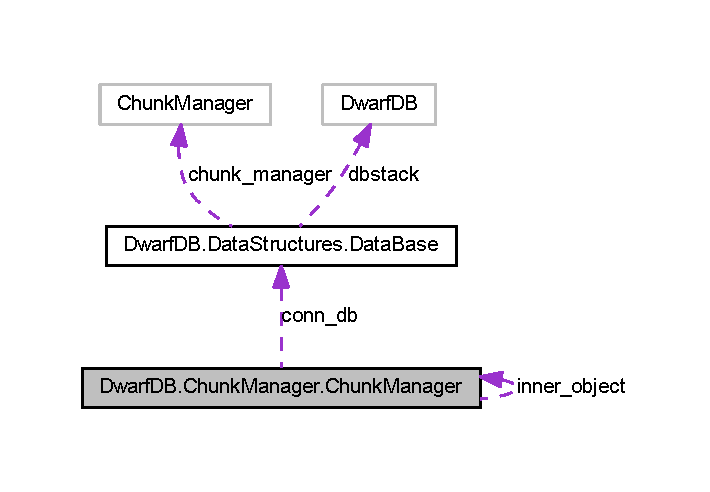
\includegraphics[width=341pt]{class_dwarf_d_b_1_1_chunk_manager_1_1_chunk_manager__coll__graph}
\end{center}
\end{figure}
\subsection*{Public Member Functions}
\begin{DoxyCompactItemize}
\item 
void \hyperlink{class_dwarf_d_b_1_1_chunk_manager_1_1_chunk_manager_a607e45973d9d32b61e0f18edb09f1229}{Load} (string db\+\_\+name, bool is\+\_\+new\+\_\+db)
\begin{DoxyCompactList}\small\item\em Loading chunks list \end{DoxyCompactList}\item 
\hypertarget{class_dwarf_d_b_1_1_chunk_manager_1_1_chunk_manager_a8be3a24a6c82e512d0eb547affa86701}{List$<$ \hyperlink{class_dwarf_d_b_1_1_data_structures_1_1_record}{Record} $>$ {\bfseries Load\+Chunk} (int chunk\+\_\+number, string dc\+\_\+hash)}\label{class_dwarf_d_b_1_1_chunk_manager_1_1_chunk_manager_a8be3a24a6c82e512d0eb547affa86701}

\item 
\hypertarget{class_dwarf_d_b_1_1_chunk_manager_1_1_chunk_manager_a8b2837bcd58aba42d46cf9327a6563fb}{List$<$ \hyperlink{class_dwarf_d_b_1_1_data_structures_1_1_record}{Record} $>$ {\bfseries Load\+All\+Chunks} (string dc\+\_\+hash)}\label{class_dwarf_d_b_1_1_chunk_manager_1_1_chunk_manager_a8b2837bcd58aba42d46cf9327a6563fb}

\item 
void \hyperlink{class_dwarf_d_b_1_1_chunk_manager_1_1_chunk_manager_a88c934e118ea03cdc8e99290f65a967a}{Create\+Chunk} (\hyperlink{class_dwarf_d_b_1_1_data_structures_1_1_data_base}{Data\+Base} db)
\begin{DoxyCompactList}\small\item\em Creates a new chunk for databases \end{DoxyCompactList}\item 
void \hyperlink{class_dwarf_d_b_1_1_chunk_manager_1_1_chunk_manager_a9cc2ba0706faf8e49af4a098f0ffffd5}{Create\+Chunk} (\hyperlink{class_dwarf_d_b_1_1_data_structures_1_1_data_container}{Data\+Container} dc)
\begin{DoxyCompactList}\small\item\em Creates a new chunk for data containers \end{DoxyCompactList}\item 
void \hyperlink{class_dwarf_d_b_1_1_chunk_manager_1_1_chunk_manager_a96ab6bd09f2a5b1d05fe92163e40b512}{Create\+Chunk} (List$<$ \hyperlink{class_dwarf_d_b_1_1_data_structures_1_1_record}{Record} $>$ records, int max\+\_\+elem\+\_\+count=100)
\begin{DoxyCompactList}\small\item\em Creates a new chunk for records \end{DoxyCompactList}\item 
\hyperlink{class_dwarf_d_b_1_1_data_structures_1_1_data_container}{Data\+Container} \hyperlink{class_dwarf_d_b_1_1_chunk_manager_1_1_chunk_manager_ae7fb3a97ffa480b023785dfca48e18ec}{Get\+Data\+Container} (string dc\+\_\+name)
\begin{DoxyCompactList}\small\item\em Searching a Data Container by name \end{DoxyCompactList}\item 
\hyperlink{class_dwarf_d_b_1_1_data_structures_1_1_data_container}{Data\+Container} \hyperlink{class_dwarf_d_b_1_1_chunk_manager_1_1_chunk_manager_ac7362867e884632398fb26cf4f0ef9b5}{Get\+Data\+Container} (\hyperlink{class_dwarf_d_b_1_1_data_structures_1_1_index}{Index} dc\+\_\+index)
\begin{DoxyCompactList}\small\item\em Searching a Data Container by index \end{DoxyCompactList}\item 
\hyperlink{class_dwarf_d_b_1_1_data_structures_1_1_record}{Record} \hyperlink{class_dwarf_d_b_1_1_chunk_manager_1_1_chunk_manager_a188cdde83cc43cef01aabe0fd998f16f}{Get\+Record} (\hyperlink{class_dwarf_d_b_1_1_data_structures_1_1_index}{Index} rec\+\_\+index)
\begin{DoxyCompactList}\small\item\em Searching a Record by index \end{DoxyCompactList}\item 
\hyperlink{class_dwarf_d_b_1_1_data_structures_1_1_record}{Record} \hyperlink{class_dwarf_d_b_1_1_chunk_manager_1_1_chunk_manager_a12bbf90b25cfa5ee7861e20ef6319710}{Get\+Record} (string hash)
\begin{DoxyCompactList}\small\item\em Searching a Record by index \end{DoxyCompactList}\item 
List$<$ \hyperlink{class_dwarf_d_b_1_1_data_structures_1_1_record}{Record} $>$ \hyperlink{class_dwarf_d_b_1_1_chunk_manager_1_1_chunk_manager_a037839674d8248cade1ea666c9200d9f}{Get\+Records} (List$<$ \hyperlink{class_dwarf_d_b_1_1_data_structures_1_1_index}{Index} $>$ rec\+\_\+idxs)
\begin{DoxyCompactList}\small\item\em Getting records for a Data\+Container \end{DoxyCompactList}\item 
\hypertarget{class_dwarf_d_b_1_1_chunk_manager_1_1_chunk_manager_a80aab988ea4c69f7abcfcd2015623a9c}{void {\bfseries Load\+Record\+Indexes} ()}\label{class_dwarf_d_b_1_1_chunk_manager_1_1_chunk_manager_a80aab988ea4c69f7abcfcd2015623a9c}

\item 
void \hyperlink{class_dwarf_d_b_1_1_chunk_manager_1_1_chunk_manager_af8099b5fa9a87264defdb4687e9851b0}{Save\+Indexes} ()
\begin{DoxyCompactList}\small\item\em Saves all indexes in format Name\+:\+Type\+:Index\+Hash \end{DoxyCompactList}\end{DoxyCompactItemize}
\subsection*{Static Public Member Functions}
\begin{DoxyCompactItemize}
\item 
static \hyperlink{class_dwarf_d_b_1_1_chunk_manager_1_1_chunk_manager}{Chunk\+Manager} \hyperlink{class_dwarf_d_b_1_1_chunk_manager_1_1_chunk_manager_ac75fd758d8a6f1579eb15ac3f398c1ea}{Create} (string db\+\_\+to\+\_\+connect)
\begin{DoxyCompactList}\small\item\em Creating new chunk manager for given D\+B \end{DoxyCompactList}\end{DoxyCompactItemize}
\subsection*{Static Public Attributes}
\begin{DoxyCompactItemize}
\item 
\hypertarget{class_dwarf_d_b_1_1_chunk_manager_1_1_chunk_manager_a43d4aebedbb50fdfeb27840b3aa4849b}{static \hyperlink{class_dwarf_d_b_1_1_chunk_manager_1_1_chunk_manager}{Chunk\+Manager} {\bfseries inner\+\_\+object} = null}\label{class_dwarf_d_b_1_1_chunk_manager_1_1_chunk_manager_a43d4aebedbb50fdfeb27840b3aa4849b}

\end{DoxyCompactItemize}
\subsection*{Properties}
\begin{DoxyCompactItemize}
\item 
\hypertarget{class_dwarf_d_b_1_1_chunk_manager_1_1_chunk_manager_ab3d1c419f8c1c396ca43368f5f214614}{string {\bfseries Current\+Db\+Path}\hspace{0.3cm}{\ttfamily  \mbox{[}get\mbox{]}}}\label{class_dwarf_d_b_1_1_chunk_manager_1_1_chunk_manager_ab3d1c419f8c1c396ca43368f5f214614}

\item 
\hypertarget{class_dwarf_d_b_1_1_chunk_manager_1_1_chunk_manager_a9adc3ce8d62f6341303c48e8dae3cc17}{Dictionary$<$ \hyperlink{class_dwarf_d_b_1_1_data_structures_1_1_index}{Index}, \\*
Key\+Value\+Pair$<$ \hyperlink{interface_dwarf_d_b_1_1_data_structures_1_1_i_structure}{I\+Structure}, \\*
string $>$ $>$ {\bfseries All\+Indexes}\hspace{0.3cm}{\ttfamily  \mbox{[}get\mbox{]}}}\label{class_dwarf_d_b_1_1_chunk_manager_1_1_chunk_manager_a9adc3ce8d62f6341303c48e8dae3cc17}

\end{DoxyCompactItemize}


\subsection{Detailed Description}
Description of \hyperlink{class_dwarf_d_b_1_1_chunk_manager_1_1_chunk_manager}{Chunk\+Manager}. 



\subsection{Member Function Documentation}
\hypertarget{class_dwarf_d_b_1_1_chunk_manager_1_1_chunk_manager_ac75fd758d8a6f1579eb15ac3f398c1ea}{\index{Dwarf\+D\+B\+::\+Chunk\+Manager\+::\+Chunk\+Manager@{Dwarf\+D\+B\+::\+Chunk\+Manager\+::\+Chunk\+Manager}!Create@{Create}}
\index{Create@{Create}!Dwarf\+D\+B\+::\+Chunk\+Manager\+::\+Chunk\+Manager@{Dwarf\+D\+B\+::\+Chunk\+Manager\+::\+Chunk\+Manager}}
\subsubsection[{Create}]{\setlength{\rightskip}{0pt plus 5cm}static {\bf Chunk\+Manager} Dwarf\+D\+B.\+Chunk\+Manager.\+Chunk\+Manager.\+Create (
\begin{DoxyParamCaption}
\item[{string}]{db\+\_\+to\+\_\+connect}
\end{DoxyParamCaption}
)\hspace{0.3cm}{\ttfamily [static]}}}\label{class_dwarf_d_b_1_1_chunk_manager_1_1_chunk_manager_ac75fd758d8a6f1579eb15ac3f398c1ea}


Creating new chunk manager for given D\+B 


\begin{DoxyParams}{Parameters}
{\em db\+\_\+to\+\_\+connect} & D\+B name\\
\hline
\end{DoxyParams}
\begin{DoxyReturn}{Returns}

\end{DoxyReturn}
\hypertarget{class_dwarf_d_b_1_1_chunk_manager_1_1_chunk_manager_a88c934e118ea03cdc8e99290f65a967a}{\index{Dwarf\+D\+B\+::\+Chunk\+Manager\+::\+Chunk\+Manager@{Dwarf\+D\+B\+::\+Chunk\+Manager\+::\+Chunk\+Manager}!Create\+Chunk@{Create\+Chunk}}
\index{Create\+Chunk@{Create\+Chunk}!Dwarf\+D\+B\+::\+Chunk\+Manager\+::\+Chunk\+Manager@{Dwarf\+D\+B\+::\+Chunk\+Manager\+::\+Chunk\+Manager}}
\subsubsection[{Create\+Chunk}]{\setlength{\rightskip}{0pt plus 5cm}void Dwarf\+D\+B.\+Chunk\+Manager.\+Chunk\+Manager.\+Create\+Chunk (
\begin{DoxyParamCaption}
\item[{{\bf Data\+Base}}]{db}
\end{DoxyParamCaption}
)}}\label{class_dwarf_d_b_1_1_chunk_manager_1_1_chunk_manager_a88c934e118ea03cdc8e99290f65a967a}


Creates a new chunk for databases 


\begin{DoxyParams}{Parameters}
{\em db} & Database\\
\hline
\end{DoxyParams}
\hypertarget{class_dwarf_d_b_1_1_chunk_manager_1_1_chunk_manager_a9cc2ba0706faf8e49af4a098f0ffffd5}{\index{Dwarf\+D\+B\+::\+Chunk\+Manager\+::\+Chunk\+Manager@{Dwarf\+D\+B\+::\+Chunk\+Manager\+::\+Chunk\+Manager}!Create\+Chunk@{Create\+Chunk}}
\index{Create\+Chunk@{Create\+Chunk}!Dwarf\+D\+B\+::\+Chunk\+Manager\+::\+Chunk\+Manager@{Dwarf\+D\+B\+::\+Chunk\+Manager\+::\+Chunk\+Manager}}
\subsubsection[{Create\+Chunk}]{\setlength{\rightskip}{0pt plus 5cm}void Dwarf\+D\+B.\+Chunk\+Manager.\+Chunk\+Manager.\+Create\+Chunk (
\begin{DoxyParamCaption}
\item[{{\bf Data\+Container}}]{dc}
\end{DoxyParamCaption}
)}}\label{class_dwarf_d_b_1_1_chunk_manager_1_1_chunk_manager_a9cc2ba0706faf8e49af4a098f0ffffd5}


Creates a new chunk for data containers 


\begin{DoxyParams}{Parameters}
{\em dc} & Data\+Container\\
\hline
\end{DoxyParams}


Here is the call graph for this function\+:


\hypertarget{class_dwarf_d_b_1_1_chunk_manager_1_1_chunk_manager_a96ab6bd09f2a5b1d05fe92163e40b512}{\index{Dwarf\+D\+B\+::\+Chunk\+Manager\+::\+Chunk\+Manager@{Dwarf\+D\+B\+::\+Chunk\+Manager\+::\+Chunk\+Manager}!Create\+Chunk@{Create\+Chunk}}
\index{Create\+Chunk@{Create\+Chunk}!Dwarf\+D\+B\+::\+Chunk\+Manager\+::\+Chunk\+Manager@{Dwarf\+D\+B\+::\+Chunk\+Manager\+::\+Chunk\+Manager}}
\subsubsection[{Create\+Chunk}]{\setlength{\rightskip}{0pt plus 5cm}void Dwarf\+D\+B.\+Chunk\+Manager.\+Chunk\+Manager.\+Create\+Chunk (
\begin{DoxyParamCaption}
\item[{List$<$ {\bf Record} $>$}]{records, }
\item[{int}]{max\+\_\+elem\+\_\+count = {\ttfamily 100}}
\end{DoxyParamCaption}
)}}\label{class_dwarf_d_b_1_1_chunk_manager_1_1_chunk_manager_a96ab6bd09f2a5b1d05fe92163e40b512}


Creates a new chunk for records 


\begin{DoxyParams}{Parameters}
{\em last\+\_\+new\+\_\+elems\+\_\+count} & A count of new elements to put in new chunk( if needed! )\\
\hline
{\em max\+\_\+idx\+\_\+count} & \\
\hline
\end{DoxyParams}


Here is the call graph for this function\+:


\hypertarget{class_dwarf_d_b_1_1_chunk_manager_1_1_chunk_manager_ae7fb3a97ffa480b023785dfca48e18ec}{\index{Dwarf\+D\+B\+::\+Chunk\+Manager\+::\+Chunk\+Manager@{Dwarf\+D\+B\+::\+Chunk\+Manager\+::\+Chunk\+Manager}!Get\+Data\+Container@{Get\+Data\+Container}}
\index{Get\+Data\+Container@{Get\+Data\+Container}!Dwarf\+D\+B\+::\+Chunk\+Manager\+::\+Chunk\+Manager@{Dwarf\+D\+B\+::\+Chunk\+Manager\+::\+Chunk\+Manager}}
\subsubsection[{Get\+Data\+Container}]{\setlength{\rightskip}{0pt plus 5cm}{\bf Data\+Container} Dwarf\+D\+B.\+Chunk\+Manager.\+Chunk\+Manager.\+Get\+Data\+Container (
\begin{DoxyParamCaption}
\item[{string}]{dc\+\_\+name}
\end{DoxyParamCaption}
)}}\label{class_dwarf_d_b_1_1_chunk_manager_1_1_chunk_manager_ae7fb3a97ffa480b023785dfca48e18ec}


Searching a Data Container by name 


\begin{DoxyParams}{Parameters}
{\em dc\+\_\+name} & Data\+Container name\\
\hline
\end{DoxyParams}
\begin{DoxyReturn}{Returns}

\end{DoxyReturn}
\hypertarget{class_dwarf_d_b_1_1_chunk_manager_1_1_chunk_manager_ac7362867e884632398fb26cf4f0ef9b5}{\index{Dwarf\+D\+B\+::\+Chunk\+Manager\+::\+Chunk\+Manager@{Dwarf\+D\+B\+::\+Chunk\+Manager\+::\+Chunk\+Manager}!Get\+Data\+Container@{Get\+Data\+Container}}
\index{Get\+Data\+Container@{Get\+Data\+Container}!Dwarf\+D\+B\+::\+Chunk\+Manager\+::\+Chunk\+Manager@{Dwarf\+D\+B\+::\+Chunk\+Manager\+::\+Chunk\+Manager}}
\subsubsection[{Get\+Data\+Container}]{\setlength{\rightskip}{0pt plus 5cm}{\bf Data\+Container} Dwarf\+D\+B.\+Chunk\+Manager.\+Chunk\+Manager.\+Get\+Data\+Container (
\begin{DoxyParamCaption}
\item[{{\bf Index}}]{dc\+\_\+index}
\end{DoxyParamCaption}
)}}\label{class_dwarf_d_b_1_1_chunk_manager_1_1_chunk_manager_ac7362867e884632398fb26cf4f0ef9b5}


Searching a Data Container by index 


\begin{DoxyParams}{Parameters}
{\em dc\+\_\+index} & D\+C index\\
\hline
\end{DoxyParams}
\begin{DoxyReturn}{Returns}

\end{DoxyReturn}
\hypertarget{class_dwarf_d_b_1_1_chunk_manager_1_1_chunk_manager_a188cdde83cc43cef01aabe0fd998f16f}{\index{Dwarf\+D\+B\+::\+Chunk\+Manager\+::\+Chunk\+Manager@{Dwarf\+D\+B\+::\+Chunk\+Manager\+::\+Chunk\+Manager}!Get\+Record@{Get\+Record}}
\index{Get\+Record@{Get\+Record}!Dwarf\+D\+B\+::\+Chunk\+Manager\+::\+Chunk\+Manager@{Dwarf\+D\+B\+::\+Chunk\+Manager\+::\+Chunk\+Manager}}
\subsubsection[{Get\+Record}]{\setlength{\rightskip}{0pt plus 5cm}{\bf Record} Dwarf\+D\+B.\+Chunk\+Manager.\+Chunk\+Manager.\+Get\+Record (
\begin{DoxyParamCaption}
\item[{{\bf Index}}]{rec\+\_\+index}
\end{DoxyParamCaption}
)}}\label{class_dwarf_d_b_1_1_chunk_manager_1_1_chunk_manager_a188cdde83cc43cef01aabe0fd998f16f}


Searching a Record by index 


\begin{DoxyParams}{Parameters}
{\em dc\+\_\+index} & Record index\\
\hline
\end{DoxyParams}
\begin{DoxyReturn}{Returns}

\end{DoxyReturn}
\hypertarget{class_dwarf_d_b_1_1_chunk_manager_1_1_chunk_manager_a12bbf90b25cfa5ee7861e20ef6319710}{\index{Dwarf\+D\+B\+::\+Chunk\+Manager\+::\+Chunk\+Manager@{Dwarf\+D\+B\+::\+Chunk\+Manager\+::\+Chunk\+Manager}!Get\+Record@{Get\+Record}}
\index{Get\+Record@{Get\+Record}!Dwarf\+D\+B\+::\+Chunk\+Manager\+::\+Chunk\+Manager@{Dwarf\+D\+B\+::\+Chunk\+Manager\+::\+Chunk\+Manager}}
\subsubsection[{Get\+Record}]{\setlength{\rightskip}{0pt plus 5cm}{\bf Record} Dwarf\+D\+B.\+Chunk\+Manager.\+Chunk\+Manager.\+Get\+Record (
\begin{DoxyParamCaption}
\item[{string}]{hash}
\end{DoxyParamCaption}
)}}\label{class_dwarf_d_b_1_1_chunk_manager_1_1_chunk_manager_a12bbf90b25cfa5ee7861e20ef6319710}


Searching a Record by index 


\begin{DoxyParams}{Parameters}
{\em hash} & Record hashcode\\
\hline
\end{DoxyParams}
\begin{DoxyReturn}{Returns}

\end{DoxyReturn}
\hypertarget{class_dwarf_d_b_1_1_chunk_manager_1_1_chunk_manager_a037839674d8248cade1ea666c9200d9f}{\index{Dwarf\+D\+B\+::\+Chunk\+Manager\+::\+Chunk\+Manager@{Dwarf\+D\+B\+::\+Chunk\+Manager\+::\+Chunk\+Manager}!Get\+Records@{Get\+Records}}
\index{Get\+Records@{Get\+Records}!Dwarf\+D\+B\+::\+Chunk\+Manager\+::\+Chunk\+Manager@{Dwarf\+D\+B\+::\+Chunk\+Manager\+::\+Chunk\+Manager}}
\subsubsection[{Get\+Records}]{\setlength{\rightskip}{0pt plus 5cm}List$<${\bf Record}$>$ Dwarf\+D\+B.\+Chunk\+Manager.\+Chunk\+Manager.\+Get\+Records (
\begin{DoxyParamCaption}
\item[{List$<$ {\bf Index} $>$}]{rec\+\_\+idxs}
\end{DoxyParamCaption}
)}}\label{class_dwarf_d_b_1_1_chunk_manager_1_1_chunk_manager_a037839674d8248cade1ea666c9200d9f}


Getting records for a Data\+Container 


\begin{DoxyParams}{Parameters}
{\em dc\+\_\+index} & Record index\\
\hline
\end{DoxyParams}
\begin{DoxyReturn}{Returns}

\end{DoxyReturn}
\hypertarget{class_dwarf_d_b_1_1_chunk_manager_1_1_chunk_manager_a607e45973d9d32b61e0f18edb09f1229}{\index{Dwarf\+D\+B\+::\+Chunk\+Manager\+::\+Chunk\+Manager@{Dwarf\+D\+B\+::\+Chunk\+Manager\+::\+Chunk\+Manager}!Load@{Load}}
\index{Load@{Load}!Dwarf\+D\+B\+::\+Chunk\+Manager\+::\+Chunk\+Manager@{Dwarf\+D\+B\+::\+Chunk\+Manager\+::\+Chunk\+Manager}}
\subsubsection[{Load}]{\setlength{\rightskip}{0pt plus 5cm}void Dwarf\+D\+B.\+Chunk\+Manager.\+Chunk\+Manager.\+Load (
\begin{DoxyParamCaption}
\item[{string}]{db\+\_\+name, }
\item[{bool}]{is\+\_\+new\+\_\+db}
\end{DoxyParamCaption}
)}}\label{class_dwarf_d_b_1_1_chunk_manager_1_1_chunk_manager_a607e45973d9d32b61e0f18edb09f1229}


Loading chunks list 

\hypertarget{class_dwarf_d_b_1_1_chunk_manager_1_1_chunk_manager_af8099b5fa9a87264defdb4687e9851b0}{\index{Dwarf\+D\+B\+::\+Chunk\+Manager\+::\+Chunk\+Manager@{Dwarf\+D\+B\+::\+Chunk\+Manager\+::\+Chunk\+Manager}!Save\+Indexes@{Save\+Indexes}}
\index{Save\+Indexes@{Save\+Indexes}!Dwarf\+D\+B\+::\+Chunk\+Manager\+::\+Chunk\+Manager@{Dwarf\+D\+B\+::\+Chunk\+Manager\+::\+Chunk\+Manager}}
\subsubsection[{Save\+Indexes}]{\setlength{\rightskip}{0pt plus 5cm}void Dwarf\+D\+B.\+Chunk\+Manager.\+Chunk\+Manager.\+Save\+Indexes (
\begin{DoxyParamCaption}
{}
\end{DoxyParamCaption}
)}}\label{class_dwarf_d_b_1_1_chunk_manager_1_1_chunk_manager_af8099b5fa9a87264defdb4687e9851b0}


Saves all indexes in format Name\+:\+Type\+:Index\+Hash 



The documentation for this class was generated from the following file\+:\begin{DoxyCompactItemize}
\item 
Chunk\+Manager/Chunk\+Manager.\+cs\end{DoxyCompactItemize}

\hypertarget{class_dwarf_d_b_1_1_data_structures_1_1_column}{\section{Dwarf\+D\+B.\+Data\+Structures.\+Column Class Reference}
\label{class_dwarf_d_b_1_1_data_structures_1_1_column}\index{Dwarf\+D\+B.\+Data\+Structures.\+Column@{Dwarf\+D\+B.\+Data\+Structures.\+Column}}
}


Inheritance diagram for Dwarf\+D\+B.\+Data\+Structures.\+Column\+:


Collaboration diagram for Dwarf\+D\+B.\+Data\+Structures.\+Column\+:
\subsection*{Public Member Functions}
\begin{DoxyCompactItemize}
\item 
\hypertarget{class_dwarf_d_b_1_1_data_structures_1_1_column_abf5e30f6b3e6c498f0a66d02f7f17214}{{\bfseries Column} (Serialization\+Info info, Streaming\+Context ctxt)}\label{class_dwarf_d_b_1_1_data_structures_1_1_column_abf5e30f6b3e6c498f0a66d02f7f17214}

\item 
\hypertarget{class_dwarf_d_b_1_1_data_structures_1_1_column_a4a4dd5bdf12ad2ab575b62f5a4315d17}{void {\bfseries Get\+Object\+Data} (Serialization\+Info info, Streaming\+Context ctxt)}\label{class_dwarf_d_b_1_1_data_structures_1_1_column_a4a4dd5bdf12ad2ab575b62f5a4315d17}

\end{DoxyCompactItemize}
\subsection*{Properties}
\begin{DoxyCompactItemize}
\item 
\hypertarget{class_dwarf_d_b_1_1_data_structures_1_1_column_a731a4e7a643fd90916b3e54fe5712e9f}{String {\bfseries Name}\hspace{0.3cm}{\ttfamily  \mbox{[}get, set\mbox{]}}}\label{class_dwarf_d_b_1_1_data_structures_1_1_column_a731a4e7a643fd90916b3e54fe5712e9f}

\item 
\hypertarget{class_dwarf_d_b_1_1_data_structures_1_1_column_a5221d8051286c8cddc890ab614d8580a}{Data\+Type {\bfseries Type}\hspace{0.3cm}{\ttfamily  \mbox{[}get, set\mbox{]}}}\label{class_dwarf_d_b_1_1_data_structures_1_1_column_a5221d8051286c8cddc890ab614d8580a}

\end{DoxyCompactItemize}


The documentation for this class was generated from the following file\+:\begin{DoxyCompactItemize}
\item 
Data\+Structures/Data\+Container.\+cs\end{DoxyCompactItemize}

\hypertarget{class_dwarf_d_b_1_1_dwarf_command_1_1_command}{\section{Dwarf\+D\+B.\+Dwarf\+Command.\+Command Class Reference}
\label{class_dwarf_d_b_1_1_dwarf_command_1_1_command}\index{Dwarf\+D\+B.\+Dwarf\+Command.\+Command@{Dwarf\+D\+B.\+Dwarf\+Command.\+Command}}
}


Description of \hyperlink{class_dwarf_d_b_1_1_dwarf_command_1_1_command}{Command}.  




\subsection{Detailed Description}
Description of \hyperlink{class_dwarf_d_b_1_1_dwarf_command_1_1_command}{Command}. 



The documentation for this class was generated from the following file\+:\begin{DoxyCompactItemize}
\item 
Dwarf\+Command/Command.\+cs\end{DoxyCompactItemize}

\hypertarget{class_dwarf_d_b_1_1_config_1_1_config}{
\section{DwarfDB.Config.Config Class Reference}
\label{class_dwarf_d_b_1_1_config_1_1_config}\index{DwarfDB::Config::Config@{DwarfDB::Config::Config}}
}


Description of \hyperlink{class_dwarf_d_b_1_1_config_1_1_config}{Config}.  




Collaboration diagram for DwarfDB.Config.Config:\nopagebreak
\begin{figure}[H]
\begin{center}
\leavevmode
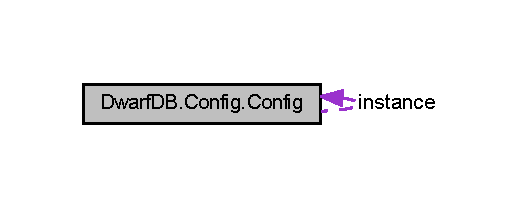
\includegraphics[width=249pt]{class_dwarf_d_b_1_1_config_1_1_config__coll__graph}
\end{center}
\end{figure}
\subsection*{Properties}
\begin{DoxyCompactItemize}
\item 
String \hyperlink{class_dwarf_d_b_1_1_config_1_1_config_afcb080c4360c0c344d2b9d9ecb72c297}{DataDirectory}\hspace{0.3cm}{\ttfamily  \mbox{[}get, set\mbox{]}}
\begin{DoxyCompactList}\small\item\em A directory for databases. \item\end{DoxyCompactList}\item 
string \hyperlink{class_dwarf_d_b_1_1_config_1_1_config_a390a89963606ed0009489bfe8b46160d}{HomePath}\hspace{0.3cm}{\ttfamily  \mbox{[}get\mbox{]}}
\begin{DoxyCompactList}\small\item\em User's HOME path. \item\end{DoxyCompactList}\item 
\hypertarget{class_dwarf_d_b_1_1_config_1_1_config_af1db0cd463b4f00c1a1b7fd4373b230a}{
static \hyperlink{class_dwarf_d_b_1_1_config_1_1_config}{Config} {\bfseries Instance}\hspace{0.3cm}{\ttfamily  \mbox{[}get\mbox{]}}}
\label{class_dwarf_d_b_1_1_config_1_1_config_af1db0cd463b4f00c1a1b7fd4373b230a}

\end{DoxyCompactItemize}


\subsection{Detailed Description}
Description of \hyperlink{class_dwarf_d_b_1_1_config_1_1_config}{Config}. 

\subsection{Property Documentation}
\hypertarget{class_dwarf_d_b_1_1_config_1_1_config_afcb080c4360c0c344d2b9d9ecb72c297}{
\index{DwarfDB::Config::Config@{DwarfDB::Config::Config}!DataDirectory@{DataDirectory}}
\index{DataDirectory@{DataDirectory}!DwarfDB::Config::Config@{DwarfDB::Config::Config}}
\subsubsection[{DataDirectory}]{\setlength{\rightskip}{0pt plus 5cm}String DwarfDB.Config.Config.DataDirectory\hspace{0.3cm}{\ttfamily  \mbox{[}get, set\mbox{]}}}}
\label{class_dwarf_d_b_1_1_config_1_1_config_afcb080c4360c0c344d2b9d9ecb72c297}


A directory for databases. 

\hypertarget{class_dwarf_d_b_1_1_config_1_1_config_a390a89963606ed0009489bfe8b46160d}{
\index{DwarfDB::Config::Config@{DwarfDB::Config::Config}!HomePath@{HomePath}}
\index{HomePath@{HomePath}!DwarfDB::Config::Config@{DwarfDB::Config::Config}}
\subsubsection[{HomePath}]{\setlength{\rightskip}{0pt plus 5cm}string DwarfDB.Config.Config.HomePath\hspace{0.3cm}{\ttfamily  \mbox{[}get\mbox{]}}}}
\label{class_dwarf_d_b_1_1_config_1_1_config_a390a89963606ed0009489bfe8b46160d}


User's HOME path. 



The documentation for this class was generated from the following file:\begin{DoxyCompactItemize}
\item 
Config/Config.cs\end{DoxyCompactItemize}

\hypertarget{class_dwarf_d_b_1_1_data_structures_1_1_data_base}{\section{Dwarf\+D\+B.\+Data\+Structures.\+Data\+Base Class Reference}
\label{class_dwarf_d_b_1_1_data_structures_1_1_data_base}\index{Dwarf\+D\+B.\+Data\+Structures.\+Data\+Base@{Dwarf\+D\+B.\+Data\+Structures.\+Data\+Base}}
}


a class for database object  




Inheritance diagram for Dwarf\+D\+B.\+Data\+Structures.\+Data\+Base\+:


Collaboration diagram for Dwarf\+D\+B.\+Data\+Structures.\+Data\+Base\+:\nopagebreak
\begin{figure}[H]
\begin{center}
\leavevmode
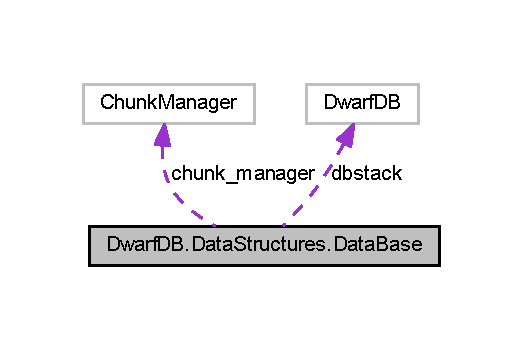
\includegraphics[width=248pt]{class_dwarf_d_b_1_1_data_structures_1_1_data_base__coll__graph}
\end{center}
\end{figure}
\subsection*{Public Member Functions}
\begin{DoxyCompactItemize}
\item 
\hypertarget{class_dwarf_d_b_1_1_data_structures_1_1_data_base_a9748f9609030f61d1cfc28a162a48ad5}{{\bfseries Data\+Base} (Serialization\+Info info, Streaming\+Context ctxt)}\label{class_dwarf_d_b_1_1_data_structures_1_1_data_base_a9748f9609030f61d1cfc28a162a48ad5}

\item 
\hypertarget{class_dwarf_d_b_1_1_data_structures_1_1_data_base_a34980ba6f61e15d6dcbe5af7f596a6fd}{void {\bfseries Get\+Object\+Data} (Serialization\+Info info, Streaming\+Context ctxt)}\label{class_dwarf_d_b_1_1_data_structures_1_1_data_base_a34980ba6f61e15d6dcbe5af7f596a6fd}

\item 
\hypertarget{class_dwarf_d_b_1_1_data_structures_1_1_data_base_ae169105e97a66c5d621b3d945d11fce4}{void {\bfseries Drop} ()}\label{class_dwarf_d_b_1_1_data_structures_1_1_data_base_ae169105e97a66c5d621b3d945d11fce4}

\item 
bool \hyperlink{class_dwarf_d_b_1_1_data_structures_1_1_data_base_af1cedf55fdab7efe9154ea7570c9abc9}{Clone\+Data\+Container} (\hyperlink{class_dwarf_d_b_1_1_data_structures_1_1_data_base}{Data\+Base} from, String dc\+\_\+name)
\begin{DoxyCompactList}\small\item\em Cloning D\+C from another D\+B \end{DoxyCompactList}\item 
\hypertarget{class_dwarf_d_b_1_1_data_structures_1_1_data_base_ae0180400ee59265e19a5d981f59ca440}{void {\bfseries Connect} (\hyperlink{class_dwarf_d_b_1_1_user_1_1_user}{User.\+User} user)}\label{class_dwarf_d_b_1_1_data_structures_1_1_data_base_ae0180400ee59265e19a5d981f59ca440}

\item 
\hypertarget{class_dwarf_d_b_1_1_data_structures_1_1_data_base_a251d5fa0ba9b21d911a9a1c5dcf33152}{bool {\bfseries Add\+New\+Data\+Container} (\hyperlink{class_dwarf_d_b_1_1_data_structures_1_1_data_container}{Data\+Container} new\+\_\+dc)}\label{class_dwarf_d_b_1_1_data_structures_1_1_data_base_a251d5fa0ba9b21d911a9a1c5dcf33152}

\item 
\hyperlink{class_dwarf_d_b_1_1_data_structures_1_1_data_container}{Data\+Container} \hyperlink{class_dwarf_d_b_1_1_data_structures_1_1_data_base_aa554e79937460eb937b90d81093019b5}{Get\+Data\+Container} (string dc\+\_\+name)
\begin{DoxyCompactList}\small\item\em Getting \hyperlink{class_dwarf_d_b_1_1_data_structures_1_1_data_container}{Data\+Container} by name \end{DoxyCompactList}\end{DoxyCompactItemize}
\subsection*{Static Public Member Functions}
\begin{DoxyCompactItemize}
\item 
\hypertarget{class_dwarf_d_b_1_1_data_structures_1_1_data_base_ace80fe82a351705958326c8d2a7f03ff}{static \hyperlink{class_dwarf_d_b_1_1_data_structures_1_1_data_base}{Data\+Base} {\bfseries Create} (string db\+\_\+name, \hyperlink{class_dwarf_d_b_1_1_chunk_manager_1_1_chunk_manager}{Chunk\+Manager.\+Chunk\+Manager} \+\_\+cm)}\label{class_dwarf_d_b_1_1_data_structures_1_1_data_base_ace80fe82a351705958326c8d2a7f03ff}

\item 
\hypertarget{class_dwarf_d_b_1_1_data_structures_1_1_data_base_af709d60f64dc5065a95dc678ebc03f30}{static \hyperlink{class_dwarf_d_b_1_1_data_structures_1_1_data_base}{Data\+Base} {\bfseries Load\+From} (string db\+\_\+name, \hyperlink{class_dwarf_d_b_1_1_chunk_manager_1_1_chunk_manager}{Chunk\+Manager.\+Chunk\+Manager} \+\_\+cm)}\label{class_dwarf_d_b_1_1_data_structures_1_1_data_base_af709d60f64dc5065a95dc678ebc03f30}

\end{DoxyCompactItemize}
\subsection*{Public Attributes}
\begin{DoxyCompactItemize}
\item 
\hypertarget{class_dwarf_d_b_1_1_data_structures_1_1_data_base_a8ccf11a71c383f6f1ac6870022a261c3}{\hyperlink{class_dwarf_d_b_1_1_chunk_manager_1_1_chunk_manager}{Chunk\+Manager.\+Chunk\+Manager} {\bfseries chunk\+\_\+manager}}\label{class_dwarf_d_b_1_1_data_structures_1_1_data_base_a8ccf11a71c383f6f1ac6870022a261c3}

\end{DoxyCompactItemize}
\subsection*{Protected Member Functions}
\begin{DoxyCompactItemize}
\item 
\hypertarget{class_dwarf_d_b_1_1_data_structures_1_1_data_base_ab2fe1cc1e8d59bbc68ad1f996507c4ee}{{\bfseries Data\+Base} (string db\+\_\+name, \hyperlink{class_dwarf_d_b_1_1_chunk_manager_1_1_chunk_manager}{Chunk\+Manager.\+Chunk\+Manager} \+\_\+cm, bool is\+\_\+new\+\_\+db)}\label{class_dwarf_d_b_1_1_data_structures_1_1_data_base_ab2fe1cc1e8d59bbc68ad1f996507c4ee}

\item 
bool \hyperlink{class_dwarf_d_b_1_1_data_structures_1_1_data_base_a5eefaebdb94adf4d3b19f29e8f146725}{Transmit} (ref \hyperlink{class_dwarf_d_b_1_1_data_structures_1_1_data_container}{Data\+Container} clone\+\_\+dc, String dn\+\_\+name)
\begin{DoxyCompactList}\small\item\em Transmitting a cloned \hyperlink{class_dwarf_d_b_1_1_data_structures_1_1_data_container}{Data\+Container} object to Recipient \end{DoxyCompactList}\end{DoxyCompactItemize}
\subsection*{Properties}
\begin{DoxyCompactItemize}
\item 
\hypertarget{class_dwarf_d_b_1_1_data_structures_1_1_data_base_a6d2cec1036e84cf7bd32e14cb57fb2c9}{string {\bfseries Db\+Path}\hspace{0.3cm}{\ttfamily  \mbox{[}get\mbox{]}}}\label{class_dwarf_d_b_1_1_data_structures_1_1_data_base_a6d2cec1036e84cf7bd32e14cb57fb2c9}

\item 
\hypertarget{class_dwarf_d_b_1_1_data_structures_1_1_data_base_a17e9d903646d5709103eabea2113c974}{Dictionary$<$ \hyperlink{class_dwarf_d_b_1_1_data_structures_1_1_index}{Index}, \\*
Key\+Value\+Pair$<$ \hyperlink{interface_dwarf_d_b_1_1_data_structures_1_1_i_structure}{I\+Structure}, \\*
string $>$ $>$ {\bfseries Indexes}\hspace{0.3cm}{\ttfamily  \mbox{[}get\mbox{]}}}\label{class_dwarf_d_b_1_1_data_structures_1_1_data_base_a17e9d903646d5709103eabea2113c974}

\item 
\hypertarget{class_dwarf_d_b_1_1_data_structures_1_1_data_base_ab8b85389f822faa790eaf18a7fe35cce}{string {\bfseries Name}\hspace{0.3cm}{\ttfamily  \mbox{[}get\mbox{]}}}\label{class_dwarf_d_b_1_1_data_structures_1_1_data_base_ab8b85389f822faa790eaf18a7fe35cce}

\item 
\hypertarget{class_dwarf_d_b_1_1_data_structures_1_1_data_base_a2ca4a32633cc1324190d6f37da17cc8b}{\hyperlink{class_dwarf_d_b_1_1_stack_1_1_dwarf_stack}{Stack.\+Dwarf\+Stack} {\bfseries Stack}\hspace{0.3cm}{\ttfamily  \mbox{[}get\mbox{]}}}\label{class_dwarf_d_b_1_1_data_structures_1_1_data_base_a2ca4a32633cc1324190d6f37da17cc8b}

\end{DoxyCompactItemize}


\subsection{Detailed Description}
a class for database object 



\subsection{Member Function Documentation}
\hypertarget{class_dwarf_d_b_1_1_data_structures_1_1_data_base_af1cedf55fdab7efe9154ea7570c9abc9}{\index{Dwarf\+D\+B\+::\+Data\+Structures\+::\+Data\+Base@{Dwarf\+D\+B\+::\+Data\+Structures\+::\+Data\+Base}!Clone\+Data\+Container@{Clone\+Data\+Container}}
\index{Clone\+Data\+Container@{Clone\+Data\+Container}!Dwarf\+D\+B\+::\+Data\+Structures\+::\+Data\+Base@{Dwarf\+D\+B\+::\+Data\+Structures\+::\+Data\+Base}}
\subsubsection[{Clone\+Data\+Container}]{\setlength{\rightskip}{0pt plus 5cm}bool Dwarf\+D\+B.\+Data\+Structures.\+Data\+Base.\+Clone\+Data\+Container (
\begin{DoxyParamCaption}
\item[{{\bf Data\+Base}}]{from, }
\item[{String}]{dc\+\_\+name}
\end{DoxyParamCaption}
)}}\label{class_dwarf_d_b_1_1_data_structures_1_1_data_base_af1cedf55fdab7efe9154ea7570c9abc9}


Cloning D\+C from another D\+B 


\begin{DoxyParams}{Parameters}
{\em from} & D\+B-\/transmitter\\
\hline
{\em dc\+\_\+name} & D\+C name to clone\\
\hline
\end{DoxyParams}
\begin{DoxyReturn}{Returns}

\end{DoxyReturn}
\hypertarget{class_dwarf_d_b_1_1_data_structures_1_1_data_base_aa554e79937460eb937b90d81093019b5}{\index{Dwarf\+D\+B\+::\+Data\+Structures\+::\+Data\+Base@{Dwarf\+D\+B\+::\+Data\+Structures\+::\+Data\+Base}!Get\+Data\+Container@{Get\+Data\+Container}}
\index{Get\+Data\+Container@{Get\+Data\+Container}!Dwarf\+D\+B\+::\+Data\+Structures\+::\+Data\+Base@{Dwarf\+D\+B\+::\+Data\+Structures\+::\+Data\+Base}}
\subsubsection[{Get\+Data\+Container}]{\setlength{\rightskip}{0pt plus 5cm}{\bf Data\+Container} Dwarf\+D\+B.\+Data\+Structures.\+Data\+Base.\+Get\+Data\+Container (
\begin{DoxyParamCaption}
\item[{string}]{dc\+\_\+name}
\end{DoxyParamCaption}
)}}\label{class_dwarf_d_b_1_1_data_structures_1_1_data_base_aa554e79937460eb937b90d81093019b5}


Getting \hyperlink{class_dwarf_d_b_1_1_data_structures_1_1_data_container}{Data\+Container} by name 


\begin{DoxyParams}{Parameters}
{\em dc\+\_\+name} & D\+C name\\
\hline
\end{DoxyParams}
\begin{DoxyReturn}{Returns}

\end{DoxyReturn}
\hypertarget{class_dwarf_d_b_1_1_data_structures_1_1_data_base_a5eefaebdb94adf4d3b19f29e8f146725}{\index{Dwarf\+D\+B\+::\+Data\+Structures\+::\+Data\+Base@{Dwarf\+D\+B\+::\+Data\+Structures\+::\+Data\+Base}!Transmit@{Transmit}}
\index{Transmit@{Transmit}!Dwarf\+D\+B\+::\+Data\+Structures\+::\+Data\+Base@{Dwarf\+D\+B\+::\+Data\+Structures\+::\+Data\+Base}}
\subsubsection[{Transmit}]{\setlength{\rightskip}{0pt plus 5cm}bool Dwarf\+D\+B.\+Data\+Structures.\+Data\+Base.\+Transmit (
\begin{DoxyParamCaption}
\item[{ref {\bf Data\+Container}}]{clone\+\_\+dc, }
\item[{String}]{dn\+\_\+name}
\end{DoxyParamCaption}
)\hspace{0.3cm}{\ttfamily [protected]}}}\label{class_dwarf_d_b_1_1_data_structures_1_1_data_base_a5eefaebdb94adf4d3b19f29e8f146725}


Transmitting a cloned \hyperlink{class_dwarf_d_b_1_1_data_structures_1_1_data_container}{Data\+Container} object to Recipient 


\begin{DoxyParams}{Parameters}
{\em clone\+\_\+dc} & Where can we put a new cloned D\+C?\\
\hline
{\em dn\+\_\+name} & D\+C name to clone\\
\hline
\end{DoxyParams}
\begin{DoxyReturn}{Returns}

\end{DoxyReturn}


The documentation for this class was generated from the following file\+:\begin{DoxyCompactItemize}
\item 
Data\+Structures/Data\+Base.\+cs\end{DoxyCompactItemize}

\hypertarget{class_dwarf_d_b_1_1_data_structures_1_1_data_base_exception}{
\section{DwarfDB.DataStructures.DataBaseException Class Reference}
\label{class_dwarf_d_b_1_1_data_structures_1_1_data_base_exception}\index{DwarfDB::DataStructures::DataBaseException@{DwarfDB::DataStructures::DataBaseException}}
}


Inheritance diagram for DwarfDB.DataStructures.DataBaseException:
\nopagebreak
\begin{figure}[H]
\begin{center}
\leavevmode
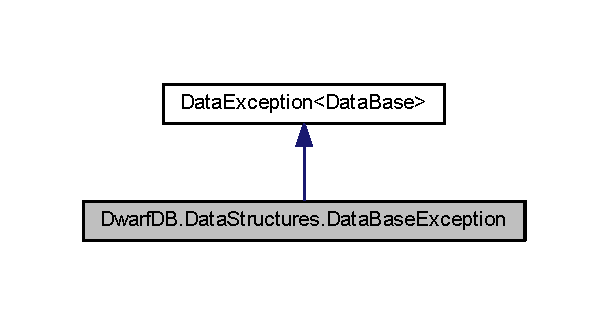
\includegraphics[width=292pt]{class_dwarf_d_b_1_1_data_structures_1_1_data_base_exception__inherit__graph}
\end{center}
\end{figure}


Collaboration diagram for DwarfDB.DataStructures.DataBaseException:
\nopagebreak
\begin{figure}[H]
\begin{center}
\leavevmode
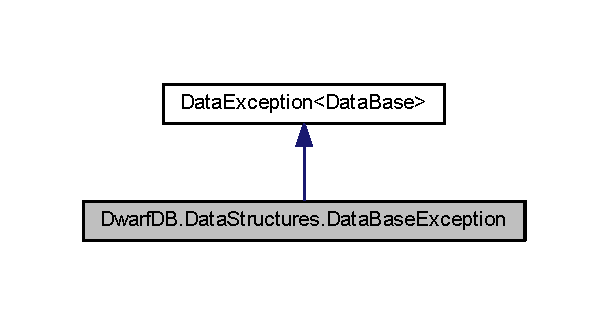
\includegraphics[width=292pt]{class_dwarf_d_b_1_1_data_structures_1_1_data_base_exception__coll__graph}
\end{center}
\end{figure}
\subsection*{Public Member Functions}
\begin{DoxyCompactItemize}
\item 
\hypertarget{class_dwarf_d_b_1_1_data_structures_1_1_data_base_exception_ac31189f613083b06927c5b7b62a5415a}{
{\bfseries DataBaseException} (string reason)}
\label{class_dwarf_d_b_1_1_data_structures_1_1_data_base_exception_ac31189f613083b06927c5b7b62a5415a}

\item 
\hypertarget{class_dwarf_d_b_1_1_data_structures_1_1_data_base_exception_a92e1a400cd2702fd38385c374478981e}{
{\bfseries DataBaseException} (\hyperlink{class_dwarf_d_b_1_1_data_structures_1_1_data_base}{DataBase} \_\-object, string reason)}
\label{class_dwarf_d_b_1_1_data_structures_1_1_data_base_exception_a92e1a400cd2702fd38385c374478981e}

\end{DoxyCompactItemize}


The documentation for this class was generated from the following file:\begin{DoxyCompactItemize}
\item 
DataStructures/DataException.cs\end{DoxyCompactItemize}

\hypertarget{class_dwarf_d_b_1_1_unit_tests_1_1_data_base_test}{\section{Dwarf\+D\+B.\+Unit\+Tests.\+Data\+Base\+Test Class Reference}
\label{class_dwarf_d_b_1_1_unit_tests_1_1_data_base_test}\index{Dwarf\+D\+B.\+Unit\+Tests.\+Data\+Base\+Test@{Dwarf\+D\+B.\+Unit\+Tests.\+Data\+Base\+Test}}
}
\subsection*{Public Member Functions}
\begin{DoxyCompactItemize}
\item 
\hypertarget{class_dwarf_d_b_1_1_unit_tests_1_1_data_base_test_a3dccc953d20e97fa83507fa9958c20c7}{void {\bfseries Drop} ()}\label{class_dwarf_d_b_1_1_unit_tests_1_1_data_base_test_a3dccc953d20e97fa83507fa9958c20c7}

\item 
\hypertarget{class_dwarf_d_b_1_1_unit_tests_1_1_data_base_test_a6bd7caf149d6611d8dca8c1013cc1612}{void {\bfseries Create\+Container} ()}\label{class_dwarf_d_b_1_1_unit_tests_1_1_data_base_test_a6bd7caf149d6611d8dca8c1013cc1612}

\end{DoxyCompactItemize}
\subsection*{Static Public Member Functions}
\begin{DoxyCompactItemize}
\item 
\hypertarget{class_dwarf_d_b_1_1_unit_tests_1_1_data_base_test_a770bbf91e34112392e2385ea183ca7ee}{static void {\bfseries Create} ()}\label{class_dwarf_d_b_1_1_unit_tests_1_1_data_base_test_a770bbf91e34112392e2385ea183ca7ee}

\end{DoxyCompactItemize}


The documentation for this class was generated from the following file\+:\begin{DoxyCompactItemize}
\item 
Unit\+Tests/Data\+Base\+Test.\+cs\end{DoxyCompactItemize}

\hypertarget{class_dwarf_d_b_1_1_data_structures_1_1_data_container}{
\section{DwarfDB.DataStructures.DataContainer Class Reference}
\label{class_dwarf_d_b_1_1_data_structures_1_1_data_container}\index{DwarfDB::DataStructures::DataContainer@{DwarfDB::DataStructures::DataContainer}}
}


\hyperlink{class_dwarf_d_b_1_1_data_structures_1_1_data_container}{DataContainer} is the base element of DwarfDB data structure.  




Inheritance diagram for DwarfDB.DataStructures.DataContainer:
\nopagebreak
\begin{figure}[H]
\begin{center}
\leavevmode
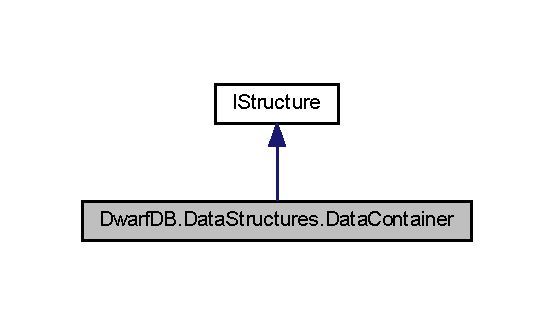
\includegraphics[width=266pt]{class_dwarf_d_b_1_1_data_structures_1_1_data_container__inherit__graph}
\end{center}
\end{figure}


Collaboration diagram for DwarfDB.DataStructures.DataContainer:
\nopagebreak
\begin{figure}[H]
\begin{center}
\leavevmode
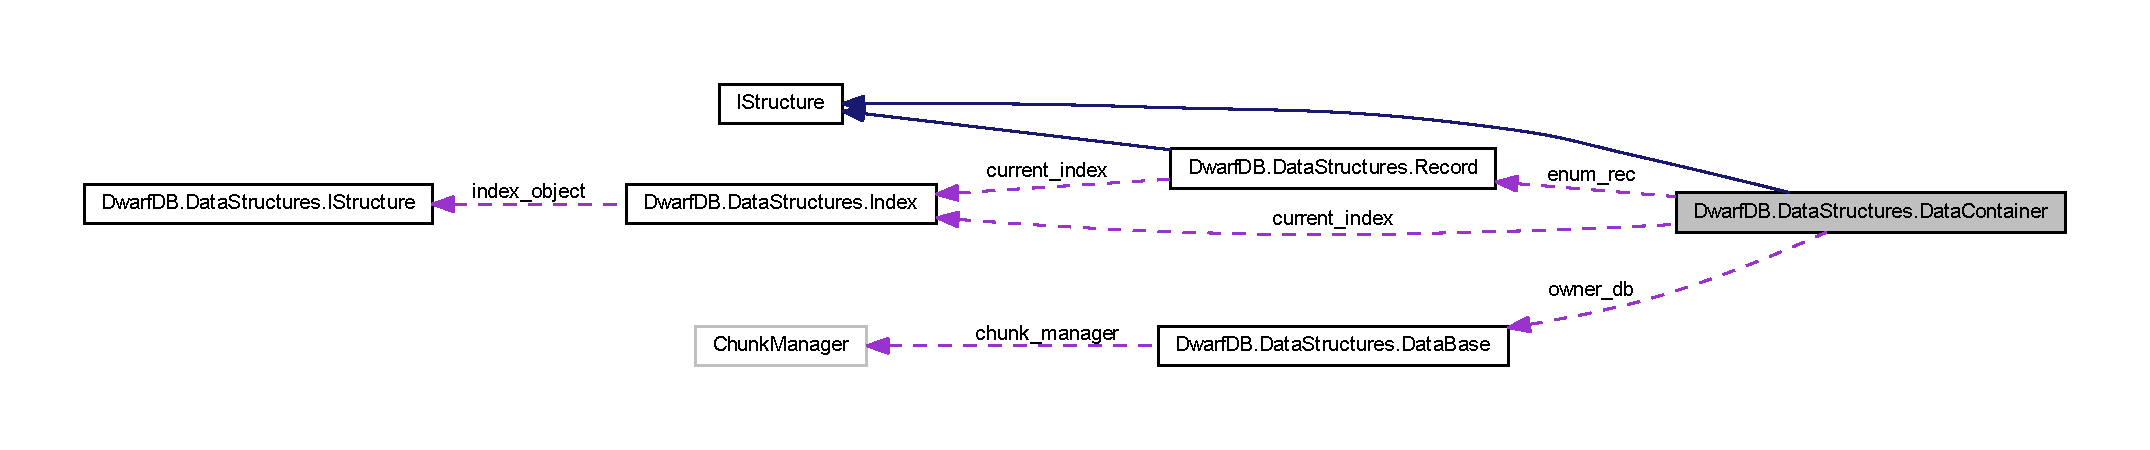
\includegraphics[width=400pt]{class_dwarf_d_b_1_1_data_structures_1_1_data_container__coll__graph}
\end{center}
\end{figure}
\subsection*{Public Member Functions}
\begin{DoxyCompactItemize}
\item 
\hypertarget{class_dwarf_d_b_1_1_data_structures_1_1_data_container_aaef12033ab5b4b00fde86e41f4bfece2}{
{\bfseries DataContainer} (\hyperlink{class_dwarf_d_b_1_1_data_structures_1_1_data_base}{DataBase} \_\-owner\_\-db, string \_\-dc\_\-name)}
\label{class_dwarf_d_b_1_1_data_structures_1_1_data_container_aaef12033ab5b4b00fde86e41f4bfece2}

\item 
\hypertarget{class_dwarf_d_b_1_1_data_structures_1_1_data_container_aedc4383268fbcc1f26b90e013cb9480a}{
{\bfseries DataContainer} (SerializationInfo info, StreamingContext ctxt)}
\label{class_dwarf_d_b_1_1_data_structures_1_1_data_container_aedc4383268fbcc1f26b90e013cb9480a}

\item 
\hypertarget{class_dwarf_d_b_1_1_data_structures_1_1_data_container_a2b870066d9ec71502d57a034c8beb610}{
void {\bfseries GetObjectData} (SerializationInfo info, StreamingContext ctxt)}
\label{class_dwarf_d_b_1_1_data_structures_1_1_data_container_a2b870066d9ec71502d57a034c8beb610}

\item 
\hypertarget{class_dwarf_d_b_1_1_data_structures_1_1_data_container_a6cb4a4c31f7e46f814632fc161024ac1}{
override bool {\bfseries Equals} (System.Object obj)}
\label{class_dwarf_d_b_1_1_data_structures_1_1_data_container_a6cb4a4c31f7e46f814632fc161024ac1}

\item 
\hypertarget{class_dwarf_d_b_1_1_data_structures_1_1_data_container_a5f7fad1592467a438632e9351ec124fa}{
override int {\bfseries GetHashCode} ()}
\label{class_dwarf_d_b_1_1_data_structures_1_1_data_container_a5f7fad1592467a438632e9351ec124fa}

\item 
void \hyperlink{class_dwarf_d_b_1_1_data_structures_1_1_data_container_aa5a712b9a8923f2d57278b58d46d6927}{LoadRecords} ()
\begin{DoxyCompactList}\small\item\em Loading all records from chunks. \item\end{DoxyCompactList}\item 
bool \hyperlink{class_dwarf_d_b_1_1_data_structures_1_1_data_container_ac2f044ee93ae6a4ba25b0deb9333867e}{AddNextCoupleOfRecords} (int number=20)
\begin{DoxyCompactList}\small\item\em Adding a next couple of records to stack. \item\end{DoxyCompactList}\item 
bool \hyperlink{class_dwarf_d_b_1_1_data_structures_1_1_data_container_accdc07066ac67d50fe891f8768e734b9}{Create} (String new\_\-name, \hyperlink{class_dwarf_d_b_1_1_data_structures_1_1_column}{Column}\mbox{[}$\,$\mbox{]} \_\-columns)
\begin{DoxyCompactList}\small\item\em Create new \hyperlink{class_dwarf_d_b_1_1_data_structures_1_1_data_container}{DataContainer}. \item\end{DoxyCompactList}\item 
\hypertarget{class_dwarf_d_b_1_1_data_structures_1_1_data_container_acee585ee5f3d45fe8474a03d533e9119}{
bool {\bfseries Delete} (String name)}
\label{class_dwarf_d_b_1_1_data_structures_1_1_data_container_acee585ee5f3d45fe8474a03d533e9119}

\item 
\hypertarget{class_dwarf_d_b_1_1_data_structures_1_1_data_container_a8e38284dde8d76439d691723da7f80fb}{
bool {\bfseries AddColumn} (\hyperlink{class_dwarf_d_b_1_1_data_structures_1_1_column}{Column} new\_\-clmn)}
\label{class_dwarf_d_b_1_1_data_structures_1_1_data_container_a8e38284dde8d76439d691723da7f80fb}

\item 
\hypertarget{class_dwarf_d_b_1_1_data_structures_1_1_data_container_a1430289cc6995618a055ff537c7c0d4e}{
void {\bfseries RemoveAllRecords} ()}
\label{class_dwarf_d_b_1_1_data_structures_1_1_data_container_a1430289cc6995618a055ff537c7c0d4e}

\item 
\hypertarget{class_dwarf_d_b_1_1_data_structures_1_1_data_container_ae5974df1699b7ccb5e6a41b0d86aeb85}{
bool {\bfseries RemoveRecord} (\hyperlink{class_dwarf_d_b_1_1_data_structures_1_1_record}{Record} rem\_\-rec)}
\label{class_dwarf_d_b_1_1_data_structures_1_1_data_container_ae5974df1699b7ccb5e6a41b0d86aeb85}

\item 
\hypertarget{class_dwarf_d_b_1_1_data_structures_1_1_data_container_a74ffad7564db689751c64501d644026a}{
bool {\bfseries AddRecord} (\hyperlink{class_dwarf_d_b_1_1_data_structures_1_1_record}{Record} new\_\-rec)}
\label{class_dwarf_d_b_1_1_data_structures_1_1_data_container_a74ffad7564db689751c64501d644026a}

\item 
\hypertarget{class_dwarf_d_b_1_1_data_structures_1_1_data_container_ae1018ff6ba68ea2ae75dadcc383eb1f2}{
bool {\bfseries RemoveColumn} (\hyperlink{class_dwarf_d_b_1_1_data_structures_1_1_column}{Column} new\_\-clmn)}
\label{class_dwarf_d_b_1_1_data_structures_1_1_data_container_ae1018ff6ba68ea2ae75dadcc383eb1f2}

\item 
\hypertarget{class_dwarf_d_b_1_1_data_structures_1_1_data_container_ac9a1a5d317146e5fdc6e0b5068495670}{
int {\bfseries ColumnsCount} ()}
\label{class_dwarf_d_b_1_1_data_structures_1_1_data_container_ac9a1a5d317146e5fdc6e0b5068495670}

\item 
\hypertarget{class_dwarf_d_b_1_1_data_structures_1_1_data_container_a5b1d05dc2b2b1a56c14bf3fecd26d4f0}{
int {\bfseries StackRecordsCount} ()}
\label{class_dwarf_d_b_1_1_data_structures_1_1_data_container_a5b1d05dc2b2b1a56c14bf3fecd26d4f0}

\item 
void \hyperlink{class_dwarf_d_b_1_1_data_structures_1_1_data_container_a8f32eb712d14d6dbf42a95098673dd19}{BuildIndex} ()
\begin{DoxyCompactList}\small\item\em Building an index for element. \item\end{DoxyCompactList}\item 
void \hyperlink{class_dwarf_d_b_1_1_data_structures_1_1_data_container_a3ca82caee7d6f38c74dbb4e2a637aecb}{Save} ()
\begin{DoxyCompactList}\small\item\em Save to file chunk. \item\end{DoxyCompactList}\item 
void \hyperlink{class_dwarf_d_b_1_1_data_structures_1_1_data_container_ab045853ddb62b681d2474d7e547186de}{Load} (\hyperlink{class_dwarf_d_b_1_1_data_structures_1_1_index}{Index} index)
\begin{DoxyCompactList}\small\item\em Load Element from file chunk. \item\end{DoxyCompactList}\item 
void \hyperlink{class_dwarf_d_b_1_1_data_structures_1_1_data_container_a40b2dc31b54b0d41b29e58ea5ea4a3fb}{SetTransaction} (\hyperlink{class_dwarf_d_b_1_1_transactions_1_1_dwarf_transaction}{DwarfDB.Transactions.DwarfTransaction} InTransaction)
\begin{DoxyCompactList}\small\item\em Setting up a transaction for this element. \item\end{DoxyCompactList}\item 
void \hyperlink{class_dwarf_d_b_1_1_data_structures_1_1_data_container_a0a82f79c53628134d16f2fa21db221bf}{LoadFromChunkDir} (string dirpath, \hyperlink{class_dwarf_d_b_1_1_data_structures_1_1_index}{Index} index)
\begin{DoxyCompactList}\small\item\em Load \hyperlink{class_dwarf_d_b_1_1_data_structures_1_1_data_container}{DataContainer} from file chunk directory. \item\end{DoxyCompactList}\item 
\hyperlink{class_dwarf_d_b_1_1_data_structures_1_1_data_base}{DataBase} \hyperlink{class_dwarf_d_b_1_1_data_structures_1_1_data_container_a30765f0c417065245bb4c065c7eb29e0}{GetOwnerDB} ()
\begin{DoxyCompactList}\small\item\em Getting an owner database object. \item\end{DoxyCompactList}\item 
bool \hyperlink{class_dwarf_d_b_1_1_data_structures_1_1_data_container_aeac4bb0b67fdcba42ea4933a03f295c3}{AssignOwnerDB} (\hyperlink{class_dwarf_d_b_1_1_data_structures_1_1_data_base}{DataBase} new\_\-owner)
\begin{DoxyCompactList}\small\item\em Assinging owner database object. \item\end{DoxyCompactList}\item 
\hyperlink{class_dwarf_d_b_1_1_data_structures_1_1_record}{Record} \hyperlink{class_dwarf_d_b_1_1_data_structures_1_1_data_container_afdcd349b09fa679ea11d0a04e073e965}{GetRecord} (int i)
\begin{DoxyCompactList}\small\item\em Incapsulating this.Records\mbox{[}i\mbox{]}.get for making some additional operations safely. \item\end{DoxyCompactList}\item 
List$<$ \hyperlink{class_dwarf_d_b_1_1_data_structures_1_1_record}{Record} $>$ \hyperlink{class_dwarf_d_b_1_1_data_structures_1_1_data_container_ab9691aa5445b0069bb30c4d7a9f6139c}{GetRecords} ()
\begin{DoxyCompactList}\small\item\em Getting Records. \item\end{DoxyCompactList}\item 
\hypertarget{class_dwarf_d_b_1_1_data_structures_1_1_data_container_ad72368f523f462dd3baee29e6ba4da66}{
bool {\bfseries GetRecordsFromChunk} (int chunk\_\-number=0)}
\label{class_dwarf_d_b_1_1_data_structures_1_1_data_container_ad72368f523f462dd3baee29e6ba4da66}

\item 
void \hyperlink{class_dwarf_d_b_1_1_data_structures_1_1_data_container_adb2c609dd0c1c9230ac94454a6db723f}{PreLoad} ()
\begin{DoxyCompactList}\small\item\em Method for loading all DC content into the stack. \item\end{DoxyCompactList}\item 
\hypertarget{class_dwarf_d_b_1_1_data_structures_1_1_data_container_aaea9c8cb3180484e56d0f6b47f90b23c}{
\hyperlink{class_dwarf_d_b_1_1_data_structures_1_1_record}{Record} {\bfseries GetEnumerator} ()}
\label{class_dwarf_d_b_1_1_data_structures_1_1_data_container_aaea9c8cb3180484e56d0f6b47f90b23c}

\item 
\hyperlink{interface_dwarf_d_b_1_1_data_structures_1_1_i_structure}{IStructure} \hyperlink{class_dwarf_d_b_1_1_data_structures_1_1_data_container_a246c00add5642b9674339a0319bae617}{Clone} ()
\begin{DoxyCompactList}\small\item\em Cloning procedure for DataStructure with reassigning a new owner object( for DC! ) \item\end{DoxyCompactList}\item 
\hyperlink{class_dwarf_d_b_1_1_data_structures_1_1_index}{Index} \hyperlink{class_dwarf_d_b_1_1_data_structures_1_1_data_container_a195b9a3fcaa91d3240e07164c1d5c460}{GetIndex} ()
\begin{DoxyCompactList}\small\item\em Getting an index for element. \item\end{DoxyCompactList}\end{DoxyCompactItemize}
\subsection*{Static Public Member Functions}
\begin{DoxyCompactItemize}
\item 
\hypertarget{class_dwarf_d_b_1_1_data_structures_1_1_data_container_a7a47a45e62754b629dc06c57438a4eca}{
static bool {\bfseries operator==} (\hyperlink{class_dwarf_d_b_1_1_data_structures_1_1_data_container}{DataContainer} a, \hyperlink{class_dwarf_d_b_1_1_data_structures_1_1_data_container}{DataContainer} b)}
\label{class_dwarf_d_b_1_1_data_structures_1_1_data_container_a7a47a45e62754b629dc06c57438a4eca}

\item 
\hypertarget{class_dwarf_d_b_1_1_data_structures_1_1_data_container_aa59ee6235912ea37a590efe9a147b704}{
static bool {\bfseries operator!=} (\hyperlink{class_dwarf_d_b_1_1_data_structures_1_1_data_container}{DataContainer} a, \hyperlink{class_dwarf_d_b_1_1_data_structures_1_1_data_container}{DataContainer} b)}
\label{class_dwarf_d_b_1_1_data_structures_1_1_data_container_aa59ee6235912ea37a590efe9a147b704}

\item 
static bool \hyperlink{class_dwarf_d_b_1_1_data_structures_1_1_data_container_a57324435e4d7961b4b875588b9a86f3d}{Create} (\hyperlink{class_dwarf_d_b_1_1_data_structures_1_1_data_base}{DataBase} \_\-owner\_\-db, String \_\-name)
\begin{DoxyCompactList}\small\item\em Create new \hyperlink{class_dwarf_d_b_1_1_data_structures_1_1_data_container}{DataContainer}. \item\end{DoxyCompactList}\end{DoxyCompactItemize}
\subsection*{Protected Attributes}
\begin{DoxyCompactItemize}
\item 
\hypertarget{class_dwarf_d_b_1_1_data_structures_1_1_data_container_a6523a6e2c271855c1ded8e9db3daf942}{
\hyperlink{class_dwarf_d_b_1_1_data_structures_1_1_record}{Record} {\bfseries enum\_\-rec} = null}
\label{class_dwarf_d_b_1_1_data_structures_1_1_data_container_a6523a6e2c271855c1ded8e9db3daf942}

\item 
\hypertarget{class_dwarf_d_b_1_1_data_structures_1_1_data_container_a4c471406e24d5b180e22208a1e379a23}{
int {\bfseries position} = 0}
\label{class_dwarf_d_b_1_1_data_structures_1_1_data_container_a4c471406e24d5b180e22208a1e379a23}

\item 
\hypertarget{class_dwarf_d_b_1_1_data_structures_1_1_data_container_a4f2b41475b859b75ab39c65186ac6753}{
\hyperlink{class_dwarf_d_b_1_1_data_structures_1_1_data_base}{DataBase} {\bfseries owner\_\-db}}
\label{class_dwarf_d_b_1_1_data_structures_1_1_data_container_a4f2b41475b859b75ab39c65186ac6753}

\item 
\hypertarget{class_dwarf_d_b_1_1_data_structures_1_1_data_container_a54d86d75f344d0cca8c2323143aa77b1}{
\hyperlink{class_dwarf_d_b_1_1_data_structures_1_1_index}{Index} {\bfseries current\_\-index}}
\label{class_dwarf_d_b_1_1_data_structures_1_1_data_container_a54d86d75f344d0cca8c2323143aa77b1}

\end{DoxyCompactItemize}
\subsection*{Properties}
\begin{DoxyCompactItemize}
\item 
\hypertarget{class_dwarf_d_b_1_1_data_structures_1_1_data_container_ac285de692141c079be1bce8dccebb859}{
String {\bfseries Name}\hspace{0.3cm}{\ttfamily  \mbox{[}get, set\mbox{]}}}
\label{class_dwarf_d_b_1_1_data_structures_1_1_data_container_ac285de692141c079be1bce8dccebb859}

\item 
int \hyperlink{class_dwarf_d_b_1_1_data_structures_1_1_data_container_af2f2d766cbb2729f91effb3c68fd97e0}{AllRecordsCount}\hspace{0.3cm}{\ttfamily  \mbox{[}get\mbox{]}}
\begin{DoxyCompactList}\small\item\em Outputs full amount of records, that has this DC as a parent element. \item\end{DoxyCompactList}\item 
\hypertarget{class_dwarf_d_b_1_1_data_structures_1_1_data_container_a8b12c9bac22fa5ad7d007267f06e20c1}{
\hyperlink{class_dwarf_d_b_1_1_data_structures_1_1_record}{Record} {\bfseries this} \mbox{[}int pos\mbox{]}\hspace{0.3cm}{\ttfamily  \mbox{[}get, set\mbox{]}}}
\label{class_dwarf_d_b_1_1_data_structures_1_1_data_container_a8b12c9bac22fa5ad7d007267f06e20c1}

\item 
UInt64 \hyperlink{class_dwarf_d_b_1_1_data_structures_1_1_data_container_a3e5849e957860912c9050dbd84818dfd}{Id}\hspace{0.3cm}{\ttfamily  \mbox{[}get, set\mbox{]}}
\begin{DoxyCompactList}\small\item\em Element id. \item\end{DoxyCompactList}\item 
\hypertarget{class_dwarf_d_b_1_1_data_structures_1_1_data_container_a4b7bab104009e416ea771276c2e7161a}{
List$<$ \hyperlink{class_dwarf_d_b_1_1_data_structures_1_1_column}{Column} $>$ {\bfseries Columns}\hspace{0.3cm}{\ttfamily  \mbox{[}get, set\mbox{]}}}
\label{class_dwarf_d_b_1_1_data_structures_1_1_data_container_a4b7bab104009e416ea771276c2e7161a}

\item 
\hypertarget{class_dwarf_d_b_1_1_data_structures_1_1_data_container_a04e95f117bfb96a32811e7bfeb6c7c32}{
List$<$ \hyperlink{class_dwarf_d_b_1_1_data_structures_1_1_record}{Record} $>$ {\bfseries Records}\hspace{0.3cm}{\ttfamily  \mbox{[}get, set\mbox{]}}}
\label{class_dwarf_d_b_1_1_data_structures_1_1_data_container_a04e95f117bfb96a32811e7bfeb6c7c32}

\end{DoxyCompactItemize}


\subsection{Detailed Description}
\hyperlink{class_dwarf_d_b_1_1_data_structures_1_1_data_container}{DataContainer} is the base element of DwarfDB data structure. 

\subsection{Member Function Documentation}
\hypertarget{class_dwarf_d_b_1_1_data_structures_1_1_data_container_ac2f044ee93ae6a4ba25b0deb9333867e}{
\index{DwarfDB::DataStructures::DataContainer@{DwarfDB::DataStructures::DataContainer}!AddNextCoupleOfRecords@{AddNextCoupleOfRecords}}
\index{AddNextCoupleOfRecords@{AddNextCoupleOfRecords}!DwarfDB::DataStructures::DataContainer@{DwarfDB::DataStructures::DataContainer}}
\subsubsection[{AddNextCoupleOfRecords}]{\setlength{\rightskip}{0pt plus 5cm}bool DwarfDB.DataStructures.DataContainer.AddNextCoupleOfRecords (
\begin{DoxyParamCaption}
\item[{int}]{ number = {\ttfamily 20}}
\end{DoxyParamCaption}
)}}
\label{class_dwarf_d_b_1_1_data_structures_1_1_data_container_ac2f044ee93ae6a4ba25b0deb9333867e}


Adding a next couple of records to stack. 


\begin{DoxyParams}{Parameters}
{\em number} & \\
\hline
\end{DoxyParams}
\begin{DoxyReturn}{Returns}

\end{DoxyReturn}
\hypertarget{class_dwarf_d_b_1_1_data_structures_1_1_data_container_aeac4bb0b67fdcba42ea4933a03f295c3}{
\index{DwarfDB::DataStructures::DataContainer@{DwarfDB::DataStructures::DataContainer}!AssignOwnerDB@{AssignOwnerDB}}
\index{AssignOwnerDB@{AssignOwnerDB}!DwarfDB::DataStructures::DataContainer@{DwarfDB::DataStructures::DataContainer}}
\subsubsection[{AssignOwnerDB}]{\setlength{\rightskip}{0pt plus 5cm}bool DwarfDB.DataStructures.DataContainer.AssignOwnerDB (
\begin{DoxyParamCaption}
\item[{{\bf DataBase}}]{ new\_\-owner}
\end{DoxyParamCaption}
)}}
\label{class_dwarf_d_b_1_1_data_structures_1_1_data_container_aeac4bb0b67fdcba42ea4933a03f295c3}


Assinging owner database object. 

\begin{DoxyReturn}{Returns}

\end{DoxyReturn}
\hypertarget{class_dwarf_d_b_1_1_data_structures_1_1_data_container_a8f32eb712d14d6dbf42a95098673dd19}{
\index{DwarfDB::DataStructures::DataContainer@{DwarfDB::DataStructures::DataContainer}!BuildIndex@{BuildIndex}}
\index{BuildIndex@{BuildIndex}!DwarfDB::DataStructures::DataContainer@{DwarfDB::DataStructures::DataContainer}}
\subsubsection[{BuildIndex}]{\setlength{\rightskip}{0pt plus 5cm}void DwarfDB.DataStructures.DataContainer.BuildIndex (
\begin{DoxyParamCaption}
{}
\end{DoxyParamCaption}
)}}
\label{class_dwarf_d_b_1_1_data_structures_1_1_data_container_a8f32eb712d14d6dbf42a95098673dd19}


Building an index for element. 



Implements \hyperlink{interface_dwarf_d_b_1_1_data_structures_1_1_i_structure_ae172c3eadf80027006666105c16b11ab}{DwarfDB.DataStructures.IStructure}.

\hypertarget{class_dwarf_d_b_1_1_data_structures_1_1_data_container_a246c00add5642b9674339a0319bae617}{
\index{DwarfDB::DataStructures::DataContainer@{DwarfDB::DataStructures::DataContainer}!Clone@{Clone}}
\index{Clone@{Clone}!DwarfDB::DataStructures::DataContainer@{DwarfDB::DataStructures::DataContainer}}
\subsubsection[{Clone}]{\setlength{\rightskip}{0pt plus 5cm}{\bf IStructure} DwarfDB.DataStructures.DataContainer.Clone (
\begin{DoxyParamCaption}
{}
\end{DoxyParamCaption}
)}}
\label{class_dwarf_d_b_1_1_data_structures_1_1_data_container_a246c00add5642b9674339a0319bae617}


Cloning procedure for DataStructure with reassigning a new owner object( for DC! ) 

\begin{DoxyReturn}{Returns}

\end{DoxyReturn}


Implements \hyperlink{interface_dwarf_d_b_1_1_data_structures_1_1_i_structure_a583485e1d898015ac75b952b057fb0e0}{DwarfDB.DataStructures.IStructure}.

\hypertarget{class_dwarf_d_b_1_1_data_structures_1_1_data_container_accdc07066ac67d50fe891f8768e734b9}{
\index{DwarfDB::DataStructures::DataContainer@{DwarfDB::DataStructures::DataContainer}!Create@{Create}}
\index{Create@{Create}!DwarfDB::DataStructures::DataContainer@{DwarfDB::DataStructures::DataContainer}}
\subsubsection[{Create}]{\setlength{\rightskip}{0pt plus 5cm}bool DwarfDB.DataStructures.DataContainer.Create (
\begin{DoxyParamCaption}
\item[{String}]{ new\_\-name, }
\item[{{\bf Column}\mbox{[}$\,$\mbox{]}}]{ \_\-columns}
\end{DoxyParamCaption}
)}}
\label{class_dwarf_d_b_1_1_data_structures_1_1_data_container_accdc07066ac67d50fe891f8768e734b9}


Create new \hyperlink{class_dwarf_d_b_1_1_data_structures_1_1_data_container}{DataContainer}. 


\begin{DoxyParams}{Parameters}
{\em new\_\-name} & \hyperlink{class_dwarf_d_b_1_1_data_structures_1_1_data_container}{DataContainer} name\\
\hline
{\em \_\-columns} & columns\\
\hline
\end{DoxyParams}
\begin{DoxyReturn}{Returns}
true or false
\end{DoxyReturn}
\hypertarget{class_dwarf_d_b_1_1_data_structures_1_1_data_container_a57324435e4d7961b4b875588b9a86f3d}{
\index{DwarfDB::DataStructures::DataContainer@{DwarfDB::DataStructures::DataContainer}!Create@{Create}}
\index{Create@{Create}!DwarfDB::DataStructures::DataContainer@{DwarfDB::DataStructures::DataContainer}}
\subsubsection[{Create}]{\setlength{\rightskip}{0pt plus 5cm}static bool DwarfDB.DataStructures.DataContainer.Create (
\begin{DoxyParamCaption}
\item[{{\bf DataBase}}]{ \_\-owner\_\-db, }
\item[{String}]{ \_\-name}
\end{DoxyParamCaption}
)\hspace{0.3cm}{\ttfamily  \mbox{[}static\mbox{]}}}}
\label{class_dwarf_d_b_1_1_data_structures_1_1_data_container_a57324435e4d7961b4b875588b9a86f3d}


Create new \hyperlink{class_dwarf_d_b_1_1_data_structures_1_1_data_container}{DataContainer}. 


\begin{DoxyParams}{Parameters}
{\em \_\-owner\_\-db} & Owner DB object\\
\hline
{\em \_\-name} & \hyperlink{class_dwarf_d_b_1_1_data_structures_1_1_data_container}{DataContainer} name\\
\hline
\end{DoxyParams}
\begin{DoxyReturn}{Returns}
true or false
\end{DoxyReturn}
\hypertarget{class_dwarf_d_b_1_1_data_structures_1_1_data_container_a195b9a3fcaa91d3240e07164c1d5c460}{
\index{DwarfDB::DataStructures::DataContainer@{DwarfDB::DataStructures::DataContainer}!GetIndex@{GetIndex}}
\index{GetIndex@{GetIndex}!DwarfDB::DataStructures::DataContainer@{DwarfDB::DataStructures::DataContainer}}
\subsubsection[{GetIndex}]{\setlength{\rightskip}{0pt plus 5cm}{\bf Index} DwarfDB.DataStructures.DataContainer.GetIndex (
\begin{DoxyParamCaption}
{}
\end{DoxyParamCaption}
)}}
\label{class_dwarf_d_b_1_1_data_structures_1_1_data_container_a195b9a3fcaa91d3240e07164c1d5c460}


Getting an index for element. 

\begin{DoxyReturn}{Returns}

\end{DoxyReturn}


Implements \hyperlink{interface_dwarf_d_b_1_1_data_structures_1_1_i_structure_a6fb14f0bf9df3268084bcc31dfd9c56f}{DwarfDB.DataStructures.IStructure}.

\hypertarget{class_dwarf_d_b_1_1_data_structures_1_1_data_container_a30765f0c417065245bb4c065c7eb29e0}{
\index{DwarfDB::DataStructures::DataContainer@{DwarfDB::DataStructures::DataContainer}!GetOwnerDB@{GetOwnerDB}}
\index{GetOwnerDB@{GetOwnerDB}!DwarfDB::DataStructures::DataContainer@{DwarfDB::DataStructures::DataContainer}}
\subsubsection[{GetOwnerDB}]{\setlength{\rightskip}{0pt plus 5cm}{\bf DataBase} DwarfDB.DataStructures.DataContainer.GetOwnerDB (
\begin{DoxyParamCaption}
{}
\end{DoxyParamCaption}
)}}
\label{class_dwarf_d_b_1_1_data_structures_1_1_data_container_a30765f0c417065245bb4c065c7eb29e0}


Getting an owner database object. 

\begin{DoxyReturn}{Returns}

\end{DoxyReturn}
\hypertarget{class_dwarf_d_b_1_1_data_structures_1_1_data_container_afdcd349b09fa679ea11d0a04e073e965}{
\index{DwarfDB::DataStructures::DataContainer@{DwarfDB::DataStructures::DataContainer}!GetRecord@{GetRecord}}
\index{GetRecord@{GetRecord}!DwarfDB::DataStructures::DataContainer@{DwarfDB::DataStructures::DataContainer}}
\subsubsection[{GetRecord}]{\setlength{\rightskip}{0pt plus 5cm}{\bf Record} DwarfDB.DataStructures.DataContainer.GetRecord (
\begin{DoxyParamCaption}
\item[{int}]{ i}
\end{DoxyParamCaption}
)}}
\label{class_dwarf_d_b_1_1_data_structures_1_1_data_container_afdcd349b09fa679ea11d0a04e073e965}


Incapsulating this.Records\mbox{[}i\mbox{]}.get for making some additional operations safely. 


\begin{DoxyParams}{Parameters}
{\em i} & index\\
\hline
\end{DoxyParams}
\begin{DoxyReturn}{Returns}

\end{DoxyReturn}
\hypertarget{class_dwarf_d_b_1_1_data_structures_1_1_data_container_ab9691aa5445b0069bb30c4d7a9f6139c}{
\index{DwarfDB::DataStructures::DataContainer@{DwarfDB::DataStructures::DataContainer}!GetRecords@{GetRecords}}
\index{GetRecords@{GetRecords}!DwarfDB::DataStructures::DataContainer@{DwarfDB::DataStructures::DataContainer}}
\subsubsection[{GetRecords}]{\setlength{\rightskip}{0pt plus 5cm}List$<${\bf Record}$>$ DwarfDB.DataStructures.DataContainer.GetRecords (
\begin{DoxyParamCaption}
{}
\end{DoxyParamCaption}
)}}
\label{class_dwarf_d_b_1_1_data_structures_1_1_data_container_ab9691aa5445b0069bb30c4d7a9f6139c}


Getting Records. 

\begin{DoxyReturn}{Returns}

\end{DoxyReturn}
\hypertarget{class_dwarf_d_b_1_1_data_structures_1_1_data_container_ab045853ddb62b681d2474d7e547186de}{
\index{DwarfDB::DataStructures::DataContainer@{DwarfDB::DataStructures::DataContainer}!Load@{Load}}
\index{Load@{Load}!DwarfDB::DataStructures::DataContainer@{DwarfDB::DataStructures::DataContainer}}
\subsubsection[{Load}]{\setlength{\rightskip}{0pt plus 5cm}void DwarfDB.DataStructures.DataContainer.Load (
\begin{DoxyParamCaption}
\item[{{\bf Index}}]{ index}
\end{DoxyParamCaption}
)}}
\label{class_dwarf_d_b_1_1_data_structures_1_1_data_container_ab045853ddb62b681d2474d7e547186de}


Load Element from file chunk. 


\begin{DoxyParams}{Parameters}
{\em filepath} & \\
\hline
{\em index} & \\
\hline
\end{DoxyParams}


Implements \hyperlink{interface_dwarf_d_b_1_1_data_structures_1_1_i_structure_acc1c091913384168ec50edad8b94b94b}{DwarfDB.DataStructures.IStructure}.

\hypertarget{class_dwarf_d_b_1_1_data_structures_1_1_data_container_a0a82f79c53628134d16f2fa21db221bf}{
\index{DwarfDB::DataStructures::DataContainer@{DwarfDB::DataStructures::DataContainer}!LoadFromChunkDir@{LoadFromChunkDir}}
\index{LoadFromChunkDir@{LoadFromChunkDir}!DwarfDB::DataStructures::DataContainer@{DwarfDB::DataStructures::DataContainer}}
\subsubsection[{LoadFromChunkDir}]{\setlength{\rightskip}{0pt plus 5cm}void DwarfDB.DataStructures.DataContainer.LoadFromChunkDir (
\begin{DoxyParamCaption}
\item[{string}]{ dirpath, }
\item[{{\bf Index}}]{ index}
\end{DoxyParamCaption}
)}}
\label{class_dwarf_d_b_1_1_data_structures_1_1_data_container_a0a82f79c53628134d16f2fa21db221bf}


Load \hyperlink{class_dwarf_d_b_1_1_data_structures_1_1_data_container}{DataContainer} from file chunk directory. 


\begin{DoxyParams}{Parameters}
{\em dirpath} & \\
\hline
{\em index} & \\
\hline
\end{DoxyParams}


Implements \hyperlink{interface_dwarf_d_b_1_1_data_structures_1_1_i_structure_a2e187a88a03b9e81e6e602be9329a395}{DwarfDB.DataStructures.IStructure}.

\hypertarget{class_dwarf_d_b_1_1_data_structures_1_1_data_container_aa5a712b9a8923f2d57278b58d46d6927}{
\index{DwarfDB::DataStructures::DataContainer@{DwarfDB::DataStructures::DataContainer}!LoadRecords@{LoadRecords}}
\index{LoadRecords@{LoadRecords}!DwarfDB::DataStructures::DataContainer@{DwarfDB::DataStructures::DataContainer}}
\subsubsection[{LoadRecords}]{\setlength{\rightskip}{0pt plus 5cm}void DwarfDB.DataStructures.DataContainer.LoadRecords (
\begin{DoxyParamCaption}
{}
\end{DoxyParamCaption}
)}}
\label{class_dwarf_d_b_1_1_data_structures_1_1_data_container_aa5a712b9a8923f2d57278b58d46d6927}


Loading all records from chunks. 

\hypertarget{class_dwarf_d_b_1_1_data_structures_1_1_data_container_adb2c609dd0c1c9230ac94454a6db723f}{
\index{DwarfDB::DataStructures::DataContainer@{DwarfDB::DataStructures::DataContainer}!PreLoad@{PreLoad}}
\index{PreLoad@{PreLoad}!DwarfDB::DataStructures::DataContainer@{DwarfDB::DataStructures::DataContainer}}
\subsubsection[{PreLoad}]{\setlength{\rightskip}{0pt plus 5cm}void DwarfDB.DataStructures.DataContainer.PreLoad (
\begin{DoxyParamCaption}
{}
\end{DoxyParamCaption}
)}}
\label{class_dwarf_d_b_1_1_data_structures_1_1_data_container_adb2c609dd0c1c9230ac94454a6db723f}


Method for loading all DC content into the stack. 

\hypertarget{class_dwarf_d_b_1_1_data_structures_1_1_data_container_a3ca82caee7d6f38c74dbb4e2a637aecb}{
\index{DwarfDB::DataStructures::DataContainer@{DwarfDB::DataStructures::DataContainer}!Save@{Save}}
\index{Save@{Save}!DwarfDB::DataStructures::DataContainer@{DwarfDB::DataStructures::DataContainer}}
\subsubsection[{Save}]{\setlength{\rightskip}{0pt plus 5cm}void DwarfDB.DataStructures.DataContainer.Save (
\begin{DoxyParamCaption}
{}
\end{DoxyParamCaption}
)}}
\label{class_dwarf_d_b_1_1_data_structures_1_1_data_container_a3ca82caee7d6f38c74dbb4e2a637aecb}


Save to file chunk. 



Implements \hyperlink{interface_dwarf_d_b_1_1_data_structures_1_1_i_structure_aa97bbd5250cf7456849fa6ca6ffcc0b4}{DwarfDB.DataStructures.IStructure}.

\hypertarget{class_dwarf_d_b_1_1_data_structures_1_1_data_container_a40b2dc31b54b0d41b29e58ea5ea4a3fb}{
\index{DwarfDB::DataStructures::DataContainer@{DwarfDB::DataStructures::DataContainer}!SetTransaction@{SetTransaction}}
\index{SetTransaction@{SetTransaction}!DwarfDB::DataStructures::DataContainer@{DwarfDB::DataStructures::DataContainer}}
\subsubsection[{SetTransaction}]{\setlength{\rightskip}{0pt plus 5cm}void DwarfDB.DataStructures.DataContainer.SetTransaction (
\begin{DoxyParamCaption}
\item[{{\bf DwarfDB.Transactions.DwarfTransaction}}]{ InTransaction}
\end{DoxyParamCaption}
)}}
\label{class_dwarf_d_b_1_1_data_structures_1_1_data_container_a40b2dc31b54b0d41b29e58ea5ea4a3fb}


Setting up a transaction for this element. 


\begin{DoxyParams}{Parameters}
{\em InTransaction} & \\
\hline
\end{DoxyParams}


Implements \hyperlink{interface_dwarf_d_b_1_1_data_structures_1_1_i_structure_aa89d0ecc5915538b89865bc3086d8b0a}{DwarfDB.DataStructures.IStructure}.



\subsection{Property Documentation}
\hypertarget{class_dwarf_d_b_1_1_data_structures_1_1_data_container_af2f2d766cbb2729f91effb3c68fd97e0}{
\index{DwarfDB::DataStructures::DataContainer@{DwarfDB::DataStructures::DataContainer}!AllRecordsCount@{AllRecordsCount}}
\index{AllRecordsCount@{AllRecordsCount}!DwarfDB::DataStructures::DataContainer@{DwarfDB::DataStructures::DataContainer}}
\subsubsection[{AllRecordsCount}]{\setlength{\rightskip}{0pt plus 5cm}int DwarfDB.DataStructures.DataContainer.AllRecordsCount\hspace{0.3cm}{\ttfamily  \mbox{[}get\mbox{]}}}}
\label{class_dwarf_d_b_1_1_data_structures_1_1_data_container_af2f2d766cbb2729f91effb3c68fd97e0}


Outputs full amount of records, that has this DC as a parent element. 

\hypertarget{class_dwarf_d_b_1_1_data_structures_1_1_data_container_a3e5849e957860912c9050dbd84818dfd}{
\index{DwarfDB::DataStructures::DataContainer@{DwarfDB::DataStructures::DataContainer}!Id@{Id}}
\index{Id@{Id}!DwarfDB::DataStructures::DataContainer@{DwarfDB::DataStructures::DataContainer}}
\subsubsection[{Id}]{\setlength{\rightskip}{0pt plus 5cm}UInt64 DwarfDB.DataStructures.DataContainer.Id\hspace{0.3cm}{\ttfamily  \mbox{[}get, set\mbox{]}}}}
\label{class_dwarf_d_b_1_1_data_structures_1_1_data_container_a3e5849e957860912c9050dbd84818dfd}


Element id. 



Implements \hyperlink{interface_dwarf_d_b_1_1_data_structures_1_1_i_structure_a9fab102fba11f70ab46272b53201784d}{DwarfDB.DataStructures.IStructure}.



The documentation for this class was generated from the following file:\begin{DoxyCompactItemize}
\item 
DataStructures/DataContainer.cs\end{DoxyCompactItemize}

\hypertarget{class_dwarf_d_b_1_1_unit_tests_1_1_data_container_test}{\section{Dwarf\+D\+B.\+Unit\+Tests.\+Data\+Container\+Test Class Reference}
\label{class_dwarf_d_b_1_1_unit_tests_1_1_data_container_test}\index{Dwarf\+D\+B.\+Unit\+Tests.\+Data\+Container\+Test@{Dwarf\+D\+B.\+Unit\+Tests.\+Data\+Container\+Test}}
}


The documentation for this class was generated from the following file\+:\begin{DoxyCompactItemize}
\item 
Unit\+Tests/Data\+Container\+Test.\+cs\end{DoxyCompactItemize}

\hypertarget{class_dwarf_d_b_1_1_data_structures_1_1_data_exception_3_01_t_01_4}{\section{Dwarf\+D\+B.\+Data\+Structures.\+Data\+Exception$<$ T $>$ Class Template Reference}
\label{class_dwarf_d_b_1_1_data_structures_1_1_data_exception_3_01_t_01_4}\index{Dwarf\+D\+B.\+Data\+Structures.\+Data\+Exception$<$ T $>$@{Dwarf\+D\+B.\+Data\+Structures.\+Data\+Exception$<$ T $>$}}
}


Exception for datastructures  




Inheritance diagram for Dwarf\+D\+B.\+Data\+Structures.\+Data\+Exception$<$ T $>$\+:


Collaboration diagram for Dwarf\+D\+B.\+Data\+Structures.\+Data\+Exception$<$ T $>$\+:
\subsection*{Public Member Functions}
\begin{DoxyCompactItemize}
\item 
\hypertarget{class_dwarf_d_b_1_1_data_structures_1_1_data_exception_3_01_t_01_4_af4387a96920d83cb65d7e3f16e8722e3}{{\bfseries Data\+Exception} (T \+\_\+object, string reason)}\label{class_dwarf_d_b_1_1_data_structures_1_1_data_exception_3_01_t_01_4_af4387a96920d83cb65d7e3f16e8722e3}

\item 
\hypertarget{class_dwarf_d_b_1_1_data_structures_1_1_data_exception_3_01_t_01_4_ad5c6e96cce65e0b685f01cb18e97360a}{{\bfseries Data\+Exception} (string reason)}\label{class_dwarf_d_b_1_1_data_structures_1_1_data_exception_3_01_t_01_4_ad5c6e96cce65e0b685f01cb18e97360a}

\item 
\hypertarget{class_dwarf_d_b_1_1_data_structures_1_1_data_exception_3_01_t_01_4_a800b1e19b9ca32978883d206a8c9683e}{{\bfseries Data\+Exception} (T \+\_\+object, string reason, Exception inner\+Exception)}\label{class_dwarf_d_b_1_1_data_structures_1_1_data_exception_3_01_t_01_4_a800b1e19b9ca32978883d206a8c9683e}

\end{DoxyCompactItemize}
\subsection*{Protected Member Functions}
\begin{DoxyCompactItemize}
\item 
\hypertarget{class_dwarf_d_b_1_1_data_structures_1_1_data_exception_3_01_t_01_4_a23f040d93fb5573f115041b9bfc4d75e}{{\bfseries Data\+Exception} (Serialization\+Info info, Streaming\+Context context)}\label{class_dwarf_d_b_1_1_data_structures_1_1_data_exception_3_01_t_01_4_a23f040d93fb5573f115041b9bfc4d75e}

\end{DoxyCompactItemize}
\subsection*{Properties}
\begin{DoxyCompactItemize}
\item 
\hypertarget{class_dwarf_d_b_1_1_data_structures_1_1_data_exception_3_01_t_01_4_a0ac0e2172d354ec3554b28959a9b7772}{T {\bfseries Object}\hspace{0.3cm}{\ttfamily  \mbox{[}get\mbox{]}}}\label{class_dwarf_d_b_1_1_data_structures_1_1_data_exception_3_01_t_01_4_a0ac0e2172d354ec3554b28959a9b7772}

\item 
\hypertarget{class_dwarf_d_b_1_1_data_structures_1_1_data_exception_3_01_t_01_4_a4d68408ff2bb7810d4ece2764efc1d1c}{Date\+Time {\bfseries When}\hspace{0.3cm}{\ttfamily  \mbox{[}get\mbox{]}}}\label{class_dwarf_d_b_1_1_data_structures_1_1_data_exception_3_01_t_01_4_a4d68408ff2bb7810d4ece2764efc1d1c}

\end{DoxyCompactItemize}


\subsection{Detailed Description}
Exception for datastructures 



The documentation for this class was generated from the following file\+:\begin{DoxyCompactItemize}
\item 
Data\+Structures/Data\+Exception.\+cs\end{DoxyCompactItemize}

\hypertarget{class_dwarf_d_b_1_1_stack_1_1_data_stack_exception}{\section{Dwarf\+D\+B.\+Stack.\+Data\+Stack\+Exception Class Reference}
\label{class_dwarf_d_b_1_1_stack_1_1_data_stack_exception}\index{Dwarf\+D\+B.\+Stack.\+Data\+Stack\+Exception@{Dwarf\+D\+B.\+Stack.\+Data\+Stack\+Exception}}
}


Exception for data stacks  




Inheritance diagram for Dwarf\+D\+B.\+Stack.\+Data\+Stack\+Exception\+:


Collaboration diagram for Dwarf\+D\+B.\+Stack.\+Data\+Stack\+Exception\+:
\subsection*{Public Member Functions}
\begin{DoxyCompactItemize}
\item 
\hypertarget{class_dwarf_d_b_1_1_stack_1_1_data_stack_exception_a75bf91637eb6790f89577fe4dfb2cd66}{{\bfseries Data\+Stack\+Exception} (string reason)}\label{class_dwarf_d_b_1_1_stack_1_1_data_stack_exception_a75bf91637eb6790f89577fe4dfb2cd66}

\item 
\hypertarget{class_dwarf_d_b_1_1_stack_1_1_data_stack_exception_af6f022a09792030b2be0c07c87b9fe28}{{\bfseries Data\+Stack\+Exception} (string reason, Exception inner\+Exception)}\label{class_dwarf_d_b_1_1_stack_1_1_data_stack_exception_af6f022a09792030b2be0c07c87b9fe28}

\end{DoxyCompactItemize}
\subsection*{Protected Member Functions}
\begin{DoxyCompactItemize}
\item 
\hypertarget{class_dwarf_d_b_1_1_stack_1_1_data_stack_exception_a456baab589d0eb986f916b47ddd076d2}{{\bfseries Data\+Stack\+Exception} (Serialization\+Info info, Streaming\+Context context)}\label{class_dwarf_d_b_1_1_stack_1_1_data_stack_exception_a456baab589d0eb986f916b47ddd076d2}

\end{DoxyCompactItemize}
\subsection*{Properties}
\begin{DoxyCompactItemize}
\item 
\hypertarget{class_dwarf_d_b_1_1_stack_1_1_data_stack_exception_ab7fefbe501011036a2cc3d59ccb42cd8}{Date\+Time {\bfseries When}\hspace{0.3cm}{\ttfamily  \mbox{[}get\mbox{]}}}\label{class_dwarf_d_b_1_1_stack_1_1_data_stack_exception_ab7fefbe501011036a2cc3d59ccb42cd8}

\end{DoxyCompactItemize}


\subsection{Detailed Description}
Exception for data stacks 



The documentation for this class was generated from the following file\+:\begin{DoxyCompactItemize}
\item 
Stack/Dwarf\+Stack.\+cs\end{DoxyCompactItemize}

\hypertarget{class_dwarf_d_b_1_1_data_structures_1_1_d_s_access_manager}{\section{Dwarf\+D\+B.\+Data\+Structures.\+D\+S\+Access\+Manager Class Reference}
\label{class_dwarf_d_b_1_1_data_structures_1_1_d_s_access_manager}\index{Dwarf\+D\+B.\+Data\+Structures.\+D\+S\+Access\+Manager@{Dwarf\+D\+B.\+Data\+Structures.\+D\+S\+Access\+Manager}}
}


Description of \hyperlink{class_dwarf_d_b_1_1_data_structures_1_1_d_s_access_manager}{D\+S\+Access\+Manager}.  




Inheritance diagram for Dwarf\+D\+B.\+Data\+Structures.\+D\+S\+Access\+Manager\+:


Collaboration diagram for Dwarf\+D\+B.\+Data\+Structures.\+D\+S\+Access\+Manager\+:
\subsection*{Public Member Functions}
\begin{DoxyCompactItemize}
\item 
\hypertarget{class_dwarf_d_b_1_1_data_structures_1_1_d_s_access_manager_adff83f4ebe6889741a2cfae89cfb0b0c}{{\bfseries D\+S\+Access\+Manager} (object \+\_\+object)}\label{class_dwarf_d_b_1_1_data_structures_1_1_d_s_access_manager_adff83f4ebe6889741a2cfae89cfb0b0c}

\item 
void \hyperlink{class_dwarf_d_b_1_1_data_structures_1_1_d_s_access_manager_aea02ec1b0fac076177a798c71701178e}{Add\+Access} (\hyperlink{class_dwarf_d_b_1_1_user_1_1_user}{User.\+User} \+\_\+user, Dwarf\+D\+B.\+Access.\+Access.\+Access\+Level \+\_\+level)
\begin{DoxyCompactList}\small\item\em Adding a new access record for our D\+B \end{DoxyCompactList}\item 
void \hyperlink{class_dwarf_d_b_1_1_data_structures_1_1_d_s_access_manager_a1ea0d79dfc5488151f97fce43d384797}{Change\+Access} (\hyperlink{class_dwarf_d_b_1_1_user_1_1_user}{User.\+User} \+\_\+user, Access.\+Access.\+Access\+Level \+\_\+new\+\_\+level)
\begin{DoxyCompactList}\small\item\em Changing an access record for our D\+B \end{DoxyCompactList}\item 
Access.\+Access.\+Access\+Level \hyperlink{class_dwarf_d_b_1_1_data_structures_1_1_d_s_access_manager_a96628d21bb3399f062c1416374a63b8c}{Get\+Level} (\hyperlink{class_dwarf_d_b_1_1_user_1_1_user}{User.\+User} \+\_\+user)
\begin{DoxyCompactList}\small\item\em Getting an access level for a given user \end{DoxyCompactList}\item 
\hypertarget{class_dwarf_d_b_1_1_data_structures_1_1_d_s_access_manager_a9e129b021f25e5730c1226f65380275b}{bool {\bfseries Check\+Write\+Permission} (\hyperlink{class_dwarf_d_b_1_1_user_1_1_user}{User.\+User} \+\_\+user)}\label{class_dwarf_d_b_1_1_data_structures_1_1_d_s_access_manager_a9e129b021f25e5730c1226f65380275b}

\item 
\hypertarget{class_dwarf_d_b_1_1_data_structures_1_1_d_s_access_manager_acf7bf4804f9fc0883bd941751b1b7bbc}{bool {\bfseries Check\+Read\+Permission} (\hyperlink{class_dwarf_d_b_1_1_user_1_1_user}{User.\+User} \+\_\+user)}\label{class_dwarf_d_b_1_1_data_structures_1_1_d_s_access_manager_acf7bf4804f9fc0883bd941751b1b7bbc}

\item 
\hypertarget{class_dwarf_d_b_1_1_data_structures_1_1_d_s_access_manager_acd227913daa5f401d7d5ada6e543b78b}{bool {\bfseries Check\+Delete\+Permission} (\hyperlink{class_dwarf_d_b_1_1_user_1_1_user}{User.\+User} \+\_\+user)}\label{class_dwarf_d_b_1_1_data_structures_1_1_d_s_access_manager_acd227913daa5f401d7d5ada6e543b78b}

\item 
\hypertarget{class_dwarf_d_b_1_1_data_structures_1_1_d_s_access_manager_a9eecefa8fc613e5715525b17e3bc4295}{bool {\bfseries Check\+Create\+Subs\+Permission} (\hyperlink{class_dwarf_d_b_1_1_user_1_1_user}{User.\+User} \+\_\+user)}\label{class_dwarf_d_b_1_1_data_structures_1_1_d_s_access_manager_a9eecefa8fc613e5715525b17e3bc4295}

\item 
\hypertarget{class_dwarf_d_b_1_1_data_structures_1_1_d_s_access_manager_a5ff3abc378f6628d6ba7e0c5d38df38b}{bool {\bfseries Check\+Drop\+Permission} (\hyperlink{class_dwarf_d_b_1_1_user_1_1_user}{User.\+User} \+\_\+user)}\label{class_dwarf_d_b_1_1_data_structures_1_1_d_s_access_manager_a5ff3abc378f6628d6ba7e0c5d38df38b}

\end{DoxyCompactItemize}


\subsection{Detailed Description}
Description of \hyperlink{class_dwarf_d_b_1_1_data_structures_1_1_d_s_access_manager}{D\+S\+Access\+Manager}. 



\subsection{Member Function Documentation}
\hypertarget{class_dwarf_d_b_1_1_data_structures_1_1_d_s_access_manager_aea02ec1b0fac076177a798c71701178e}{\index{Dwarf\+D\+B\+::\+Data\+Structures\+::\+D\+S\+Access\+Manager@{Dwarf\+D\+B\+::\+Data\+Structures\+::\+D\+S\+Access\+Manager}!Add\+Access@{Add\+Access}}
\index{Add\+Access@{Add\+Access}!Dwarf\+D\+B\+::\+Data\+Structures\+::\+D\+S\+Access\+Manager@{Dwarf\+D\+B\+::\+Data\+Structures\+::\+D\+S\+Access\+Manager}}
\subsubsection[{Add\+Access}]{\setlength{\rightskip}{0pt plus 5cm}void Dwarf\+D\+B.\+Data\+Structures.\+D\+S\+Access\+Manager.\+Add\+Access (
\begin{DoxyParamCaption}
\item[{{\bf User.\+User}}]{\+\_\+user, }
\item[{Dwarf\+D\+B.\+Access.\+Access.\+Access\+Level}]{\+\_\+level}
\end{DoxyParamCaption}
)}}\label{class_dwarf_d_b_1_1_data_structures_1_1_d_s_access_manager_aea02ec1b0fac076177a798c71701178e}


Adding a new access record for our D\+B 


\begin{DoxyParams}{Parameters}
{\em \+\_\+user} & \\
\hline
{\em \+\_\+level} & \\
\hline
\end{DoxyParams}


Here is the caller graph for this function\+:


\hypertarget{class_dwarf_d_b_1_1_data_structures_1_1_d_s_access_manager_a1ea0d79dfc5488151f97fce43d384797}{\index{Dwarf\+D\+B\+::\+Data\+Structures\+::\+D\+S\+Access\+Manager@{Dwarf\+D\+B\+::\+Data\+Structures\+::\+D\+S\+Access\+Manager}!Change\+Access@{Change\+Access}}
\index{Change\+Access@{Change\+Access}!Dwarf\+D\+B\+::\+Data\+Structures\+::\+D\+S\+Access\+Manager@{Dwarf\+D\+B\+::\+Data\+Structures\+::\+D\+S\+Access\+Manager}}
\subsubsection[{Change\+Access}]{\setlength{\rightskip}{0pt plus 5cm}void Dwarf\+D\+B.\+Data\+Structures.\+D\+S\+Access\+Manager.\+Change\+Access (
\begin{DoxyParamCaption}
\item[{{\bf User.\+User}}]{\+\_\+user, }
\item[{Access.\+Access.\+Access\+Level}]{\+\_\+new\+\_\+level}
\end{DoxyParamCaption}
)}}\label{class_dwarf_d_b_1_1_data_structures_1_1_d_s_access_manager_a1ea0d79dfc5488151f97fce43d384797}


Changing an access record for our D\+B 


\begin{DoxyParams}{Parameters}
{\em \+\_\+user} & \\
\hline
{\em \+\_\+new\+\_\+level} & \\
\hline
\end{DoxyParams}


Here is the caller graph for this function\+:


\hypertarget{class_dwarf_d_b_1_1_data_structures_1_1_d_s_access_manager_a96628d21bb3399f062c1416374a63b8c}{\index{Dwarf\+D\+B\+::\+Data\+Structures\+::\+D\+S\+Access\+Manager@{Dwarf\+D\+B\+::\+Data\+Structures\+::\+D\+S\+Access\+Manager}!Get\+Level@{Get\+Level}}
\index{Get\+Level@{Get\+Level}!Dwarf\+D\+B\+::\+Data\+Structures\+::\+D\+S\+Access\+Manager@{Dwarf\+D\+B\+::\+Data\+Structures\+::\+D\+S\+Access\+Manager}}
\subsubsection[{Get\+Level}]{\setlength{\rightskip}{0pt plus 5cm}Access.\+Access.\+Access\+Level Dwarf\+D\+B.\+Data\+Structures.\+D\+S\+Access\+Manager.\+Get\+Level (
\begin{DoxyParamCaption}
\item[{{\bf User.\+User}}]{\+\_\+user}
\end{DoxyParamCaption}
)}}\label{class_dwarf_d_b_1_1_data_structures_1_1_d_s_access_manager_a96628d21bb3399f062c1416374a63b8c}


Getting an access level for a given user 


\begin{DoxyParams}{Parameters}
{\em \+\_\+user} & \\
\hline
\end{DoxyParams}
\begin{DoxyReturn}{Returns}

\end{DoxyReturn}


Here is the caller graph for this function\+:




The documentation for this class was generated from the following file\+:\begin{DoxyCompactItemize}
\item 
Data\+Structures/D\+S\+Access\+Manager.\+cs\end{DoxyCompactItemize}

\hypertarget{class_dwarf_d_b_1_1_data_structures_1_1_dummy_container}{\section{Dwarf\+D\+B.\+Data\+Structures.\+Dummy\+Container Class Reference}
\label{class_dwarf_d_b_1_1_data_structures_1_1_dummy_container}\index{Dwarf\+D\+B.\+Data\+Structures.\+Dummy\+Container@{Dwarf\+D\+B.\+Data\+Structures.\+Dummy\+Container}}
}


\hyperlink{class_dwarf_d_b_1_1_data_structures_1_1_dummy_container}{Dummy\+Container} class -\/ it's class for using instead of N\+U\+L\+L  




Inheritance diagram for Dwarf\+D\+B.\+Data\+Structures.\+Dummy\+Container\+:
\nopagebreak
\begin{figure}[H]
\begin{center}
\leavevmode
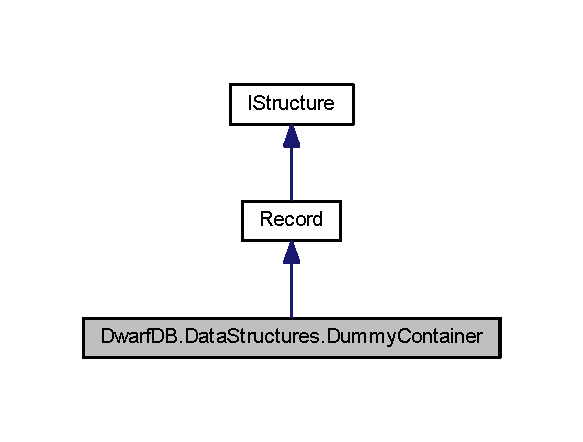
\includegraphics[width=280pt]{class_dwarf_d_b_1_1_data_structures_1_1_dummy_container__inherit__graph}
\end{center}
\end{figure}


Collaboration diagram for Dwarf\+D\+B.\+Data\+Structures.\+Dummy\+Container\+:
\nopagebreak
\begin{figure}[H]
\begin{center}
\leavevmode
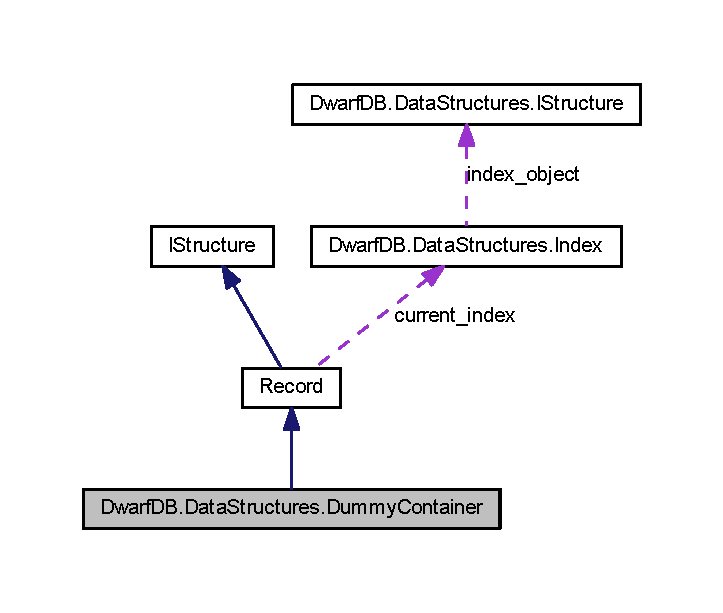
\includegraphics[width=347pt]{class_dwarf_d_b_1_1_data_structures_1_1_dummy_container__coll__graph}
\end{center}
\end{figure}
\subsection*{Public Member Functions}
\begin{DoxyCompactItemize}
\item 
\hypertarget{class_dwarf_d_b_1_1_data_structures_1_1_dummy_container_a62d4c4fe42f254e8c3072bbc4bea6fa2}{{\bfseries Dummy\+Container} (\hyperlink{class_dwarf_d_b_1_1_data_structures_1_1_data_container}{Data\+Container} \+\_\+owner\+\_\+dc)}\label{class_dwarf_d_b_1_1_data_structures_1_1_dummy_container_a62d4c4fe42f254e8c3072bbc4bea6fa2}

\end{DoxyCompactItemize}
\subsection*{Static Public Member Functions}
\begin{DoxyCompactItemize}
\item 
\hypertarget{class_dwarf_d_b_1_1_data_structures_1_1_dummy_container_a020db8f3d0bd48af1bcfba5d07e6e058}{static \hyperlink{class_dwarf_d_b_1_1_data_structures_1_1_dummy_container}{Dummy\+Container} {\bfseries Create} ()}\label{class_dwarf_d_b_1_1_data_structures_1_1_dummy_container_a020db8f3d0bd48af1bcfba5d07e6e058}

\end{DoxyCompactItemize}
\subsection*{Additional Inherited Members}


\subsection{Detailed Description}
\hyperlink{class_dwarf_d_b_1_1_data_structures_1_1_dummy_container}{Dummy\+Container} class -\/ it's class for using instead of N\+U\+L\+L 



The documentation for this class was generated from the following file\+:\begin{DoxyCompactItemize}
\item 
Data\+Structures/Dummy\+Container.\+cs\end{DoxyCompactItemize}

\hypertarget{class_dwarf_d_b_1_1_data_structures_1_1_dummy_field}{\section{Dwarf\+D\+B.\+Data\+Structures.\+Dummy\+Field Class Reference}
\label{class_dwarf_d_b_1_1_data_structures_1_1_dummy_field}\index{Dwarf\+D\+B.\+Data\+Structures.\+Dummy\+Field@{Dwarf\+D\+B.\+Data\+Structures.\+Dummy\+Field}}
}


\hyperlink{class_dwarf_d_b_1_1_data_structures_1_1_dummy_field}{Dummy\+Field} class -\/ it's class for using instead of N\+U\+L\+L  




Inheritance diagram for Dwarf\+D\+B.\+Data\+Structures.\+Dummy\+Field\+:
\nopagebreak
\begin{figure}[H]
\begin{center}
\leavevmode
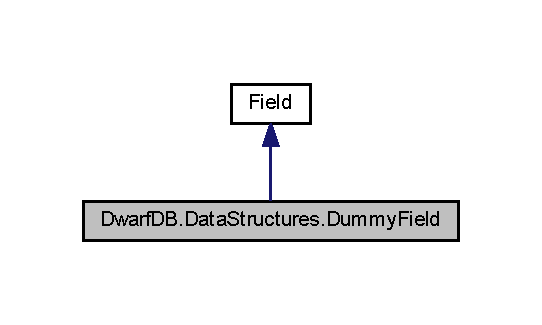
\includegraphics[width=260pt]{class_dwarf_d_b_1_1_data_structures_1_1_dummy_field__inherit__graph}
\end{center}
\end{figure}


Collaboration diagram for Dwarf\+D\+B.\+Data\+Structures.\+Dummy\+Field\+:
\nopagebreak
\begin{figure}[H]
\begin{center}
\leavevmode
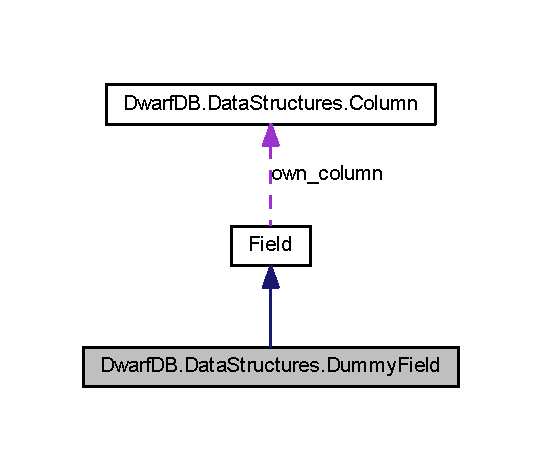
\includegraphics[width=260pt]{class_dwarf_d_b_1_1_data_structures_1_1_dummy_field__coll__graph}
\end{center}
\end{figure}
\subsection*{Static Public Member Functions}
\begin{DoxyCompactItemize}
\item 
\hypertarget{class_dwarf_d_b_1_1_data_structures_1_1_dummy_field_aa36da679dfc36a7647002ef65055cca4}{static \hyperlink{class_dwarf_d_b_1_1_data_structures_1_1_dummy_field}{Dummy\+Field} {\bfseries Create} (\hyperlink{class_dwarf_d_b_1_1_data_structures_1_1_field}{Field} example)}\label{class_dwarf_d_b_1_1_data_structures_1_1_dummy_field_aa36da679dfc36a7647002ef65055cca4}

\end{DoxyCompactItemize}
\subsection*{Additional Inherited Members}


\subsection{Detailed Description}
\hyperlink{class_dwarf_d_b_1_1_data_structures_1_1_dummy_field}{Dummy\+Field} class -\/ it's class for using instead of N\+U\+L\+L 



The documentation for this class was generated from the following file\+:\begin{DoxyCompactItemize}
\item 
Data\+Structures/Dummy\+Record.\+cs\end{DoxyCompactItemize}

\hypertarget{class_dwarf_d_b_1_1_data_structures_1_1_dummy_record}{\section{Dwarf\+D\+B.\+Data\+Structures.\+Dummy\+Record Class Reference}
\label{class_dwarf_d_b_1_1_data_structures_1_1_dummy_record}\index{Dwarf\+D\+B.\+Data\+Structures.\+Dummy\+Record@{Dwarf\+D\+B.\+Data\+Structures.\+Dummy\+Record}}
}


\hyperlink{class_dwarf_d_b_1_1_data_structures_1_1_dummy_record}{Dummy\+Record} class -\/ it's class for using instead of N\+U\+L\+L  




Inheritance diagram for Dwarf\+D\+B.\+Data\+Structures.\+Dummy\+Record\+:


Collaboration diagram for Dwarf\+D\+B.\+Data\+Structures.\+Dummy\+Record\+:
\subsection*{Public Member Functions}
\begin{DoxyCompactItemize}
\item 
\hypertarget{class_dwarf_d_b_1_1_data_structures_1_1_dummy_record_a78c4178cf8500869469b99645050e2ec}{{\bfseries Dummy\+Record} (\hyperlink{class_dwarf_d_b_1_1_data_structures_1_1_data_container}{Data\+Container} \+\_\+owner\+\_\+dc)}\label{class_dwarf_d_b_1_1_data_structures_1_1_dummy_record_a78c4178cf8500869469b99645050e2ec}

\end{DoxyCompactItemize}
\subsection*{Static Public Member Functions}
\begin{DoxyCompactItemize}
\item 
\hypertarget{class_dwarf_d_b_1_1_data_structures_1_1_dummy_record_a8fa625aa183e039b3a7c9ca365f2b7f7}{static \hyperlink{class_dwarf_d_b_1_1_data_structures_1_1_dummy_record}{Dummy\+Record} {\bfseries Create} ()}\label{class_dwarf_d_b_1_1_data_structures_1_1_dummy_record_a8fa625aa183e039b3a7c9ca365f2b7f7}

\end{DoxyCompactItemize}
\subsection*{Additional Inherited Members}


\subsection{Detailed Description}
\hyperlink{class_dwarf_d_b_1_1_data_structures_1_1_dummy_record}{Dummy\+Record} class -\/ it's class for using instead of N\+U\+L\+L 



The documentation for this class was generated from the following file\+:\begin{DoxyCompactItemize}
\item 
Data\+Structures/Dummy\+Record.\+cs\end{DoxyCompactItemize}

\hypertarget{class_dwarf_d_b_1_1_stack_1_1_dwarf_stack}{
\section{DwarfDB.Stack.DwarfStack Class Reference}
\label{class_dwarf_d_b_1_1_stack_1_1_dwarf_stack}\index{DwarfDB::Stack::DwarfStack@{DwarfDB::Stack::DwarfStack}}
}


A stack for improving an access to dwarf records.  




Collaboration diagram for DwarfDB.Stack.DwarfStack:
\nopagebreak
\begin{figure}[H]
\begin{center}
\leavevmode
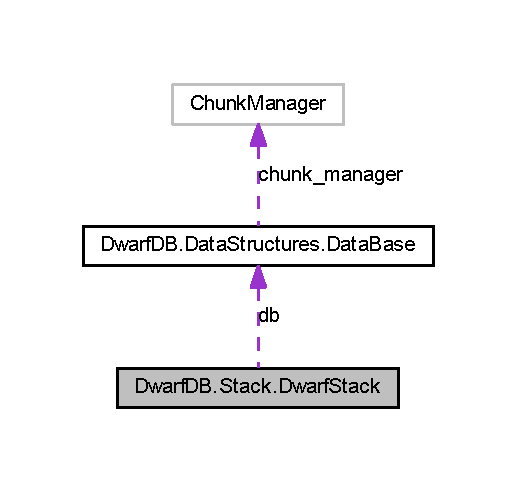
\includegraphics[width=248pt]{class_dwarf_d_b_1_1_stack_1_1_dwarf_stack__coll__graph}
\end{center}
\end{figure}
\subsection*{Public Member Functions}
\begin{DoxyCompactItemize}
\item 
\hypertarget{class_dwarf_d_b_1_1_stack_1_1_dwarf_stack_ad48677010f3ce3899b9467616fd9a7ee}{
{\bfseries DwarfStack} (\hyperlink{class_dwarf_d_b_1_1_data_structures_1_1_data_base}{DataBase} \_\-db)}
\label{class_dwarf_d_b_1_1_stack_1_1_dwarf_stack_ad48677010f3ce3899b9467616fd9a7ee}

\item 
\hypertarget{class_dwarf_d_b_1_1_stack_1_1_dwarf_stack_a885ad9cdfe63a8f8d5c55ffda79b075f}{
new void {\bfseries Push} (\hyperlink{interface_dwarf_d_b_1_1_data_structures_1_1_i_structure}{IStructure} dta\_\-struct)}
\label{class_dwarf_d_b_1_1_stack_1_1_dwarf_stack_a885ad9cdfe63a8f8d5c55ffda79b075f}

\item 
\hypertarget{class_dwarf_d_b_1_1_stack_1_1_dwarf_stack_a4b56dab4ce355bf6b5d85861d75a3ca8}{
new bool {\bfseries TryPop} (\hyperlink{interface_dwarf_d_b_1_1_data_structures_1_1_i_structure}{IStructure} data)}
\label{class_dwarf_d_b_1_1_stack_1_1_dwarf_stack_a4b56dab4ce355bf6b5d85861d75a3ca8}

\item 
\hypertarget{class_dwarf_d_b_1_1_stack_1_1_dwarf_stack_ad9a9e05a598682086956db2bfaba217a}{
bool {\bfseries ContainsHash} (string hash)}
\label{class_dwarf_d_b_1_1_stack_1_1_dwarf_stack_ad9a9e05a598682086956db2bfaba217a}

\item 
List$<$ \hyperlink{class_dwarf_d_b_1_1_data_structures_1_1_record}{Record} $>$ \hyperlink{class_dwarf_d_b_1_1_stack_1_1_dwarf_stack_adca3ef11aa4b86f2f6de7f33e06bb13c}{GetRecords} (\hyperlink{class_dwarf_d_b_1_1_data_structures_1_1_data_container}{DataStructures.DataContainer} dc)
\begin{DoxyCompactList}\small\item\em Receiving records for concrete DataContainer. \item\end{DoxyCompactList}\item 
\hyperlink{interface_dwarf_d_b_1_1_data_structures_1_1_i_structure}{IStructure} \hyperlink{class_dwarf_d_b_1_1_stack_1_1_dwarf_stack_a1cf7979ccc18a74d5a2ff3e0205ca2c7}{GetStructure} (\hyperlink{class_dwarf_d_b_1_1_data_structures_1_1_index}{Index} ind)
\begin{DoxyCompactList}\small\item\em Receiving records a record with given index. \item\end{DoxyCompactList}\end{DoxyCompactItemize}
\subsection*{Properties}
\begin{DoxyCompactItemize}
\item 
bool \hyperlink{class_dwarf_d_b_1_1_stack_1_1_dwarf_stack_a6553f7ef26d0f448c1f1833a8740b774}{Modified}\hspace{0.3cm}{\ttfamily  \mbox{[}get, set\mbox{]}}
\begin{DoxyCompactList}\small\item\em Is stack elements array modified? \item\end{DoxyCompactList}\end{DoxyCompactItemize}


\subsection{Detailed Description}
A stack for improving an access to dwarf records. 

\subsection{Member Function Documentation}
\hypertarget{class_dwarf_d_b_1_1_stack_1_1_dwarf_stack_adca3ef11aa4b86f2f6de7f33e06bb13c}{
\index{DwarfDB::Stack::DwarfStack@{DwarfDB::Stack::DwarfStack}!GetRecords@{GetRecords}}
\index{GetRecords@{GetRecords}!DwarfDB::Stack::DwarfStack@{DwarfDB::Stack::DwarfStack}}
\subsubsection[{GetRecords}]{\setlength{\rightskip}{0pt plus 5cm}List$<${\bf Record}$>$ DwarfDB.Stack.DwarfStack.GetRecords (
\begin{DoxyParamCaption}
\item[{{\bf DataStructures.DataContainer}}]{ dc}
\end{DoxyParamCaption}
)}}
\label{class_dwarf_d_b_1_1_stack_1_1_dwarf_stack_adca3ef11aa4b86f2f6de7f33e06bb13c}


Receiving records for concrete DataContainer. 


\begin{DoxyParams}{Parameters}
{\em dc} & A data container\\
\hline
\end{DoxyParams}
\begin{DoxyReturn}{Returns}

\end{DoxyReturn}
\hypertarget{class_dwarf_d_b_1_1_stack_1_1_dwarf_stack_a1cf7979ccc18a74d5a2ff3e0205ca2c7}{
\index{DwarfDB::Stack::DwarfStack@{DwarfDB::Stack::DwarfStack}!GetStructure@{GetStructure}}
\index{GetStructure@{GetStructure}!DwarfDB::Stack::DwarfStack@{DwarfDB::Stack::DwarfStack}}
\subsubsection[{GetStructure}]{\setlength{\rightskip}{0pt plus 5cm}{\bf IStructure} DwarfDB.Stack.DwarfStack.GetStructure (
\begin{DoxyParamCaption}
\item[{{\bf Index}}]{ ind}
\end{DoxyParamCaption}
)}}
\label{class_dwarf_d_b_1_1_stack_1_1_dwarf_stack_a1cf7979ccc18a74d5a2ff3e0205ca2c7}


Receiving records a record with given index. 


\begin{DoxyParams}{Parameters}
{\em ind} & \\
\hline
\end{DoxyParams}
\begin{DoxyReturn}{Returns}

\end{DoxyReturn}


\subsection{Property Documentation}
\hypertarget{class_dwarf_d_b_1_1_stack_1_1_dwarf_stack_a6553f7ef26d0f448c1f1833a8740b774}{
\index{DwarfDB::Stack::DwarfStack@{DwarfDB::Stack::DwarfStack}!Modified@{Modified}}
\index{Modified@{Modified}!DwarfDB::Stack::DwarfStack@{DwarfDB::Stack::DwarfStack}}
\subsubsection[{Modified}]{\setlength{\rightskip}{0pt plus 5cm}bool DwarfDB.Stack.DwarfStack.Modified\hspace{0.3cm}{\ttfamily  \mbox{[}get, set\mbox{]}}}}
\label{class_dwarf_d_b_1_1_stack_1_1_dwarf_stack_a6553f7ef26d0f448c1f1833a8740b774}


Is stack elements array modified? 



The documentation for this class was generated from the following file:\begin{DoxyCompactItemize}
\item 
Stack/DwarfStack.cs\end{DoxyCompactItemize}

\hypertarget{class_dwarf_d_b_1_1_transactions_1_1_dwarf_transaction}{\section{Dwarf\+D\+B.\+Transactions.\+Dwarf\+Transaction Class Reference}
\label{class_dwarf_d_b_1_1_transactions_1_1_dwarf_transaction}\index{Dwarf\+D\+B.\+Transactions.\+Dwarf\+Transaction@{Dwarf\+D\+B.\+Transactions.\+Dwarf\+Transaction}}
}


\hyperlink{class_dwarf_d_b_1_1_transactions_1_1_dwarf_transaction}{Dwarf\+Transaction} -\/ transaction without read blocking  




Inheritance diagram for Dwarf\+D\+B.\+Transactions.\+Dwarf\+Transaction\+:


Collaboration diagram for Dwarf\+D\+B.\+Transactions.\+Dwarf\+Transaction\+:
\nopagebreak
\begin{figure}[H]
\begin{center}
\leavevmode
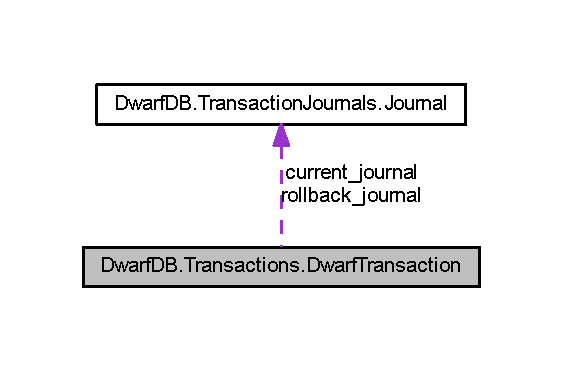
\includegraphics[width=270pt]{class_dwarf_d_b_1_1_transactions_1_1_dwarf_transaction__coll__graph}
\end{center}
\end{figure}
\subsection*{Public Member Functions}
\begin{DoxyCompactItemize}
\item 
\hypertarget{class_dwarf_d_b_1_1_transactions_1_1_dwarf_transaction_a8032193531e6c8149e201dbbbf43e956}{{\bfseries Dwarf\+Transaction} (\hyperlink{class_dwarf_d_b_1_1_dwarf_command_1_1_command}{Command} cmd)}\label{class_dwarf_d_b_1_1_transactions_1_1_dwarf_transaction_a8032193531e6c8149e201dbbbf43e956}

\item 
void \hyperlink{class_dwarf_d_b_1_1_transactions_1_1_dwarf_transaction_aa367e43159fe986df49fa72bae4548d0}{Add\+Command} (\hyperlink{class_dwarf_d_b_1_1_dwarf_command_1_1_command}{Command} cmd)
\begin{DoxyCompactList}\small\item\em Add new command into a commands queue \end{DoxyCompactList}\item 
\hypertarget{class_dwarf_d_b_1_1_transactions_1_1_dwarf_transaction_aa6901ab0d5a7bb48ad194a786c76404d}{void {\bfseries Commit} ()}\label{class_dwarf_d_b_1_1_transactions_1_1_dwarf_transaction_aa6901ab0d5a7bb48ad194a786c76404d}

\item 
\hypertarget{class_dwarf_d_b_1_1_transactions_1_1_dwarf_transaction_ae3acb0398029e288a39acc7f13877fcf}{void {\bfseries Rollback} ()}\label{class_dwarf_d_b_1_1_transactions_1_1_dwarf_transaction_ae3acb0398029e288a39acc7f13877fcf}

\item 
\hypertarget{class_dwarf_d_b_1_1_transactions_1_1_dwarf_transaction_a8cbb54489cb4d76feffcf83c23427519}{void {\bfseries Abort} ()}\label{class_dwarf_d_b_1_1_transactions_1_1_dwarf_transaction_a8cbb54489cb4d76feffcf83c23427519}

\item 
\hypertarget{class_dwarf_d_b_1_1_transactions_1_1_dwarf_transaction_a2c36e0803f86461e1833187e4140a447}{void {\bfseries Dispose} ()}\label{class_dwarf_d_b_1_1_transactions_1_1_dwarf_transaction_a2c36e0803f86461e1833187e4140a447}

\end{DoxyCompactItemize}
\subsection*{Static Public Member Functions}
\begin{DoxyCompactItemize}
\item 
static \hyperlink{class_dwarf_d_b_1_1_transactions_1_1_dwarf_transaction}{Dwarf\+Transaction} \hyperlink{class_dwarf_d_b_1_1_transactions_1_1_dwarf_transaction_a660b18b542e2053f8d8b70555ee3d5d1}{Atomic} (\hyperlink{class_dwarf_d_b_1_1_dwarf_command_1_1_command}{Command} cmd)
\begin{DoxyCompactList}\small\item\em Transaction object for atomic operations \end{DoxyCompactList}\end{DoxyCompactItemize}
\subsection*{Protected Attributes}
\begin{DoxyCompactItemize}
\item 
\hypertarget{class_dwarf_d_b_1_1_transactions_1_1_dwarf_transaction_ac669e201c78debaf241d4ae53bb8c8b6}{\hyperlink{class_dwarf_d_b_1_1_transaction_journals_1_1_journal}{Journal} {\bfseries current\+\_\+journal} = new \hyperlink{class_dwarf_d_b_1_1_transaction_journals_1_1_journal}{Journal}()}\label{class_dwarf_d_b_1_1_transactions_1_1_dwarf_transaction_ac669e201c78debaf241d4ae53bb8c8b6}

\item 
\hypertarget{class_dwarf_d_b_1_1_transactions_1_1_dwarf_transaction_a619358ab756eca4ff000419621e59aac}{\hyperlink{class_dwarf_d_b_1_1_transaction_journals_1_1_journal}{Journal} {\bfseries rollback\+\_\+journal} = new \hyperlink{class_dwarf_d_b_1_1_transaction_journals_1_1_journal}{Journal}()}\label{class_dwarf_d_b_1_1_transactions_1_1_dwarf_transaction_a619358ab756eca4ff000419621e59aac}

\item 
\hypertarget{class_dwarf_d_b_1_1_transactions_1_1_dwarf_transaction_aed2da7c0b57d388603a0c229003381bb}{Queue$<$ \hyperlink{class_dwarf_d_b_1_1_dwarf_command_1_1_command}{Command} $>$ {\bfseries commands\+\_\+chain} = new Queue$<$\hyperlink{class_dwarf_d_b_1_1_dwarf_command_1_1_command}{Command}$>$()}\label{class_dwarf_d_b_1_1_transactions_1_1_dwarf_transaction_aed2da7c0b57d388603a0c229003381bb}

\item 
\hypertarget{class_dwarf_d_b_1_1_transactions_1_1_dwarf_transaction_af7c5ad53ad36cfa8537bf9faf0c0f694}{bool {\bfseries is\+\_\+ongoing} = false}\label{class_dwarf_d_b_1_1_transactions_1_1_dwarf_transaction_af7c5ad53ad36cfa8537bf9faf0c0f694}

\item 
\hypertarget{class_dwarf_d_b_1_1_transactions_1_1_dwarf_transaction_afcb3f9b3732ab553abd49f939696178e}{bool {\bfseries is\+\_\+atomic} = false}\label{class_dwarf_d_b_1_1_transactions_1_1_dwarf_transaction_afcb3f9b3732ab553abd49f939696178e}

\end{DoxyCompactItemize}


\subsection{Detailed Description}
\hyperlink{class_dwarf_d_b_1_1_transactions_1_1_dwarf_transaction}{Dwarf\+Transaction} -\/ transaction without read blocking 



\subsection{Member Function Documentation}
\hypertarget{class_dwarf_d_b_1_1_transactions_1_1_dwarf_transaction_aa367e43159fe986df49fa72bae4548d0}{\index{Dwarf\+D\+B\+::\+Transactions\+::\+Dwarf\+Transaction@{Dwarf\+D\+B\+::\+Transactions\+::\+Dwarf\+Transaction}!Add\+Command@{Add\+Command}}
\index{Add\+Command@{Add\+Command}!Dwarf\+D\+B\+::\+Transactions\+::\+Dwarf\+Transaction@{Dwarf\+D\+B\+::\+Transactions\+::\+Dwarf\+Transaction}}
\subsubsection[{Add\+Command}]{\setlength{\rightskip}{0pt plus 5cm}void Dwarf\+D\+B.\+Transactions.\+Dwarf\+Transaction.\+Add\+Command (
\begin{DoxyParamCaption}
\item[{{\bf Command}}]{cmd}
\end{DoxyParamCaption}
)}}\label{class_dwarf_d_b_1_1_transactions_1_1_dwarf_transaction_aa367e43159fe986df49fa72bae4548d0}


Add new command into a commands queue 


\begin{DoxyParams}{Parameters}
{\em cmd} & \\
\hline
\end{DoxyParams}
\hypertarget{class_dwarf_d_b_1_1_transactions_1_1_dwarf_transaction_a660b18b542e2053f8d8b70555ee3d5d1}{\index{Dwarf\+D\+B\+::\+Transactions\+::\+Dwarf\+Transaction@{Dwarf\+D\+B\+::\+Transactions\+::\+Dwarf\+Transaction}!Atomic@{Atomic}}
\index{Atomic@{Atomic}!Dwarf\+D\+B\+::\+Transactions\+::\+Dwarf\+Transaction@{Dwarf\+D\+B\+::\+Transactions\+::\+Dwarf\+Transaction}}
\subsubsection[{Atomic}]{\setlength{\rightskip}{0pt plus 5cm}static {\bf Dwarf\+Transaction} Dwarf\+D\+B.\+Transactions.\+Dwarf\+Transaction.\+Atomic (
\begin{DoxyParamCaption}
\item[{{\bf Command}}]{cmd}
\end{DoxyParamCaption}
)\hspace{0.3cm}{\ttfamily [static]}}}\label{class_dwarf_d_b_1_1_transactions_1_1_dwarf_transaction_a660b18b542e2053f8d8b70555ee3d5d1}


Transaction object for atomic operations 

\begin{DoxyReturn}{Returns}

\end{DoxyReturn}


The documentation for this class was generated from the following file\+:\begin{DoxyCompactItemize}
\item 
Transactions/Dwarf\+Transaction.\+cs\end{DoxyCompactItemize}

\hypertarget{class_dwarf_d_b_1_1_errors_1_1_error_processing}{
\section{DwarfDB.Errors.ErrorProcessing Class Reference}
\label{class_dwarf_d_b_1_1_errors_1_1_error_processing}\index{DwarfDB::Errors::ErrorProcessing@{DwarfDB::Errors::ErrorProcessing}}
}


Description of \hyperlink{class_dwarf_d_b_1_1_errors_1_1_error_processing}{ErrorProcessing}.  


\subsection*{Static Public Member Functions}
\begin{DoxyCompactItemize}
\item 
\hypertarget{class_dwarf_d_b_1_1_errors_1_1_error_processing_a68c6bfa1f5bf2da33703992cfed77731}{
static void {\bfseries Display} (String \_\-error\_\-text, String \_\-where, String \_\-advices, DateTime date\_\-time)}
\label{class_dwarf_d_b_1_1_errors_1_1_error_processing_a68c6bfa1f5bf2da33703992cfed77731}

\item 
\hypertarget{class_dwarf_d_b_1_1_errors_1_1_error_processing_aab993dd16fc5fb11db9ef496c6aa1980}{
static void {\bfseries Display} (Stream out\_\-str, String \_\-error\_\-text, String \_\-where, String \_\-advices, DateTime date\_\-time)}
\label{class_dwarf_d_b_1_1_errors_1_1_error_processing_aab993dd16fc5fb11db9ef496c6aa1980}

\end{DoxyCompactItemize}


\subsection{Detailed Description}
Description of \hyperlink{class_dwarf_d_b_1_1_errors_1_1_error_processing}{ErrorProcessing}. 

The documentation for this class was generated from the following file:\begin{DoxyCompactItemize}
\item 
Errors/ErrorProcessing.cs\end{DoxyCompactItemize}

\hypertarget{class_dwarf_d_b_1_1_data_structures_1_1_field}{
\section{DwarfDB.DataStructures.Field Class Reference}
\label{class_dwarf_d_b_1_1_data_structures_1_1_field}\index{DwarfDB::DataStructures::Field@{DwarfDB::DataStructures::Field}}
}


Class for field of \hyperlink{class_dwarf_d_b_1_1_data_structures_1_1_record}{Record}.  




Inheritance diagram for DwarfDB.DataStructures.Field:
\nopagebreak
\begin{figure}[H]
\begin{center}
\leavevmode
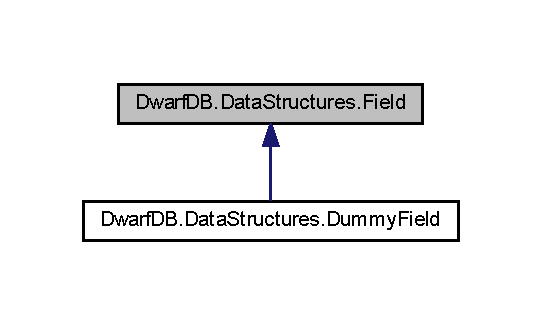
\includegraphics[width=260pt]{class_dwarf_d_b_1_1_data_structures_1_1_field__inherit__graph}
\end{center}
\end{figure}


Collaboration diagram for DwarfDB.DataStructures.Field:\nopagebreak
\begin{figure}[H]
\begin{center}
\leavevmode
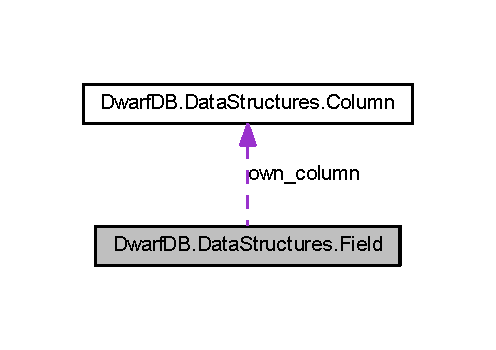
\includegraphics[width=238pt]{class_dwarf_d_b_1_1_data_structures_1_1_field__coll__graph}
\end{center}
\end{figure}
\subsection*{Public Member Functions}
\begin{DoxyCompactItemize}
\item 
\hypertarget{class_dwarf_d_b_1_1_data_structures_1_1_field_af89ec8a20b69b0f52e56c7730eb8127a}{
{\bfseries Field} (String \_\-name, DataType \_\-type, Object \_\-value)}
\label{class_dwarf_d_b_1_1_data_structures_1_1_field_af89ec8a20b69b0f52e56c7730eb8127a}

\item 
\hypertarget{class_dwarf_d_b_1_1_data_structures_1_1_field_a4772b2645a7b03be6800261db6a3c816}{
\hyperlink{class_dwarf_d_b_1_1_data_structures_1_1_field}{Field} {\bfseries Clone} ()}
\label{class_dwarf_d_b_1_1_data_structures_1_1_field_a4772b2645a7b03be6800261db6a3c816}

\end{DoxyCompactItemize}
\subsection*{Properties}
\begin{DoxyCompactItemize}
\item 
\hypertarget{class_dwarf_d_b_1_1_data_structures_1_1_field_a147e0dff27a89485bf91437d931fe5b5}{
DataType {\bfseries Type}\hspace{0.3cm}{\ttfamily  \mbox{[}get, set\mbox{]}}}
\label{class_dwarf_d_b_1_1_data_structures_1_1_field_a147e0dff27a89485bf91437d931fe5b5}

\item 
\hypertarget{class_dwarf_d_b_1_1_data_structures_1_1_field_a5c1af79be209e13f5da11e4c033f1fdb}{
String {\bfseries Name}\hspace{0.3cm}{\ttfamily  \mbox{[}get, set\mbox{]}}}
\label{class_dwarf_d_b_1_1_data_structures_1_1_field_a5c1af79be209e13f5da11e4c033f1fdb}

\item 
\hypertarget{class_dwarf_d_b_1_1_data_structures_1_1_field_ac7d7ebd43b9010ed2a7767a296e90d6f}{
Object {\bfseries Value}\hspace{0.3cm}{\ttfamily  \mbox{[}get, set\mbox{]}}}
\label{class_dwarf_d_b_1_1_data_structures_1_1_field_ac7d7ebd43b9010ed2a7767a296e90d6f}

\end{DoxyCompactItemize}


\subsection{Detailed Description}
Class for field of \hyperlink{class_dwarf_d_b_1_1_data_structures_1_1_record}{Record}. 

The documentation for this class was generated from the following file:\begin{DoxyCompactItemize}
\item 
DataStructures/Record.cs\end{DoxyCompactItemize}

\hypertarget{class_gen_key_exception}{
\section{GenKeyException Class Reference}
\label{class_gen_key_exception}\index{GenKeyException@{GenKeyException}}
}


Exception for datastructures.  


\subsection*{Public Member Functions}
\begin{DoxyCompactItemize}
\item 
\hypertarget{class_gen_key_exception_ae8de93a8f016d67c2c8cfde1fe3d15c4}{
{\bfseries GenKeyException} (string message)}
\label{class_gen_key_exception_ae8de93a8f016d67c2c8cfde1fe3d15c4}

\item 
\hypertarget{class_gen_key_exception_a89df8b04638fae6a155849d109d2189b}{
{\bfseries GenKeyException} (string message, Exception innerException)}
\label{class_gen_key_exception_a89df8b04638fae6a155849d109d2189b}

\end{DoxyCompactItemize}
\subsection*{Protected Member Functions}
\begin{DoxyCompactItemize}
\item 
\hypertarget{class_gen_key_exception_a728c2a0086dd84b7b23487b2af04e0fa}{
{\bfseries GenKeyException} (SerializationInfo info, StreamingContext context)}
\label{class_gen_key_exception_a728c2a0086dd84b7b23487b2af04e0fa}

\end{DoxyCompactItemize}


\subsection{Detailed Description}
Exception for datastructures. 

The documentation for this class was generated from the following file:\begin{DoxyCompactItemize}
\item 
Crypto/GenKeyException.cs\end{DoxyCompactItemize}

\hypertarget{class_dwarf_d_b_1_1_unit_tests_1_1_gen_key_test}{
\section{DwarfDB.UnitTests.GenKeyTest Class Reference}
\label{class_dwarf_d_b_1_1_unit_tests_1_1_gen_key_test}\index{DwarfDB::UnitTests::GenKeyTest@{DwarfDB::UnitTests::GenKeyTest}}
}
\subsection*{Public Member Functions}
\begin{DoxyCompactItemize}
\item 
\hypertarget{class_dwarf_d_b_1_1_unit_tests_1_1_gen_key_test_a0e89588b4f783127393dcc7a1d83c75c}{
void {\bfseries Generate} ()}
\label{class_dwarf_d_b_1_1_unit_tests_1_1_gen_key_test_a0e89588b4f783127393dcc7a1d83c75c}

\end{DoxyCompactItemize}


The documentation for this class was generated from the following file:\begin{DoxyCompactItemize}
\item 
UnitTests/GenKeyTest.cs\end{DoxyCompactItemize}

\hypertarget{class_dwarf_d_b_1_1_data_structures_1_1_index}{
\section{DwarfDB.DataStructures.Index Class Reference}
\label{class_dwarf_d_b_1_1_data_structures_1_1_index}\index{DwarfDB::DataStructures::Index@{DwarfDB::DataStructures::Index}}
}


\hyperlink{class_dwarf_d_b_1_1_data_structures_1_1_index}{Index} of data structure elements.  




Collaboration diagram for DwarfDB.DataStructures.Index:
\nopagebreak
\begin{figure}[H]
\begin{center}
\leavevmode
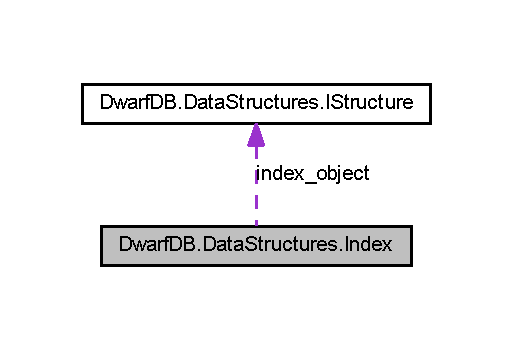
\includegraphics[width=246pt]{class_dwarf_d_b_1_1_data_structures_1_1_index__coll__graph}
\end{center}
\end{figure}
\subsection*{Public Member Functions}
\begin{DoxyCompactItemize}
\item 
\hypertarget{class_dwarf_d_b_1_1_data_structures_1_1_index_a2481d361d4dbf7cb81f094a834b93214}{
{\bfseries Index} (\hyperlink{interface_dwarf_d_b_1_1_data_structures_1_1_i_structure}{IStructure} \_\-index\_\-object)}
\label{class_dwarf_d_b_1_1_data_structures_1_1_index_a2481d361d4dbf7cb81f094a834b93214}

\item 
\hypertarget{class_dwarf_d_b_1_1_data_structures_1_1_index_aef1cd3ec762c296c9ced22ab8ed4ab12}{
override bool {\bfseries Equals} (object obj)}
\label{class_dwarf_d_b_1_1_data_structures_1_1_index_aef1cd3ec762c296c9ced22ab8ed4ab12}

\end{DoxyCompactItemize}
\subsection*{Static Public Member Functions}
\begin{DoxyCompactItemize}
\item 
\hypertarget{class_dwarf_d_b_1_1_data_structures_1_1_index_aa332f812fd66a7516a1749a6c29a04c6}{
static bool {\bfseries operator==} (\hyperlink{class_dwarf_d_b_1_1_data_structures_1_1_index}{Index} lhs, \hyperlink{class_dwarf_d_b_1_1_data_structures_1_1_index}{Index} rhs)}
\label{class_dwarf_d_b_1_1_data_structures_1_1_index_aa332f812fd66a7516a1749a6c29a04c6}

\item 
\hypertarget{class_dwarf_d_b_1_1_data_structures_1_1_index_a58d657c3d8d9fd9d122d59bf55008495}{
static bool {\bfseries operator!=} (\hyperlink{class_dwarf_d_b_1_1_data_structures_1_1_index}{Index} lhs, \hyperlink{class_dwarf_d_b_1_1_data_structures_1_1_index}{Index} rhs)}
\label{class_dwarf_d_b_1_1_data_structures_1_1_index_a58d657c3d8d9fd9d122d59bf55008495}

\item 
\hypertarget{class_dwarf_d_b_1_1_data_structures_1_1_index_a8e14d93c580e2aadd133afeef416e44a}{
static \hyperlink{class_dwarf_d_b_1_1_data_structures_1_1_index}{Index} {\bfseries CreateNew} (\hyperlink{interface_dwarf_d_b_1_1_data_structures_1_1_i_structure}{IStructure} \_\-index\_\-object)}
\label{class_dwarf_d_b_1_1_data_structures_1_1_index_a8e14d93c580e2aadd133afeef416e44a}

\item 
\hypertarget{class_dwarf_d_b_1_1_data_structures_1_1_index_affa4776e5dd06a160e8a874b0f64d769}{
static \hyperlink{class_dwarf_d_b_1_1_data_structures_1_1_index}{Index} {\bfseries CreateFromHashCode} (string hash)}
\label{class_dwarf_d_b_1_1_data_structures_1_1_index_affa4776e5dd06a160e8a874b0f64d769}

\end{DoxyCompactItemize}
\subsection*{Protected Attributes}
\begin{DoxyCompactItemize}
\item 
\hypertarget{class_dwarf_d_b_1_1_data_structures_1_1_index_a028b92bd2f8012fe81b60d0fbac93044}{
\hyperlink{interface_dwarf_d_b_1_1_data_structures_1_1_i_structure}{IStructure} {\bfseries index\_\-object}}
\label{class_dwarf_d_b_1_1_data_structures_1_1_index_a028b92bd2f8012fe81b60d0fbac93044}

\end{DoxyCompactItemize}
\subsection*{Properties}
\begin{DoxyCompactItemize}
\item 
\hypertarget{class_dwarf_d_b_1_1_data_structures_1_1_index_a610b62ec24e0fad773071dc6242eccfd}{
string {\bfseries HashCode}\hspace{0.3cm}{\ttfamily  \mbox{[}get, set\mbox{]}}}
\label{class_dwarf_d_b_1_1_data_structures_1_1_index_a610b62ec24e0fad773071dc6242eccfd}

\end{DoxyCompactItemize}


\subsection{Detailed Description}
\hyperlink{class_dwarf_d_b_1_1_data_structures_1_1_index}{Index} of data structure elements. 

The documentation for this class was generated from the following file:\begin{DoxyCompactItemize}
\item 
DataStructures/Index.cs\end{DoxyCompactItemize}

\hypertarget{class_dwarf_d_b_1_1_data_structures_1_1_index_exception}{\section{Dwarf\+D\+B.\+Data\+Structures.\+Index\+Exception Class Reference}
\label{class_dwarf_d_b_1_1_data_structures_1_1_index_exception}\index{Dwarf\+D\+B.\+Data\+Structures.\+Index\+Exception@{Dwarf\+D\+B.\+Data\+Structures.\+Index\+Exception}}
}


Inheritance diagram for Dwarf\+D\+B.\+Data\+Structures.\+Index\+Exception\+:
\nopagebreak
\begin{figure}[H]
\begin{center}
\leavevmode
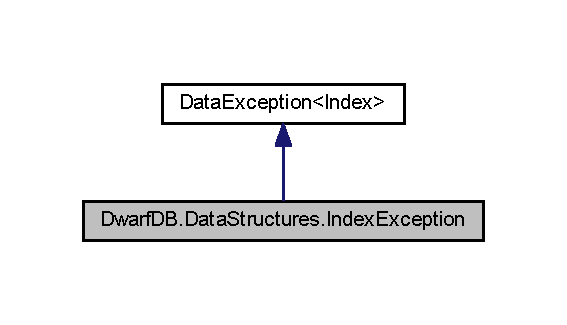
\includegraphics[width=272pt]{class_dwarf_d_b_1_1_data_structures_1_1_index_exception__inherit__graph}
\end{center}
\end{figure}


Collaboration diagram for Dwarf\+D\+B.\+Data\+Structures.\+Index\+Exception\+:
\nopagebreak
\begin{figure}[H]
\begin{center}
\leavevmode
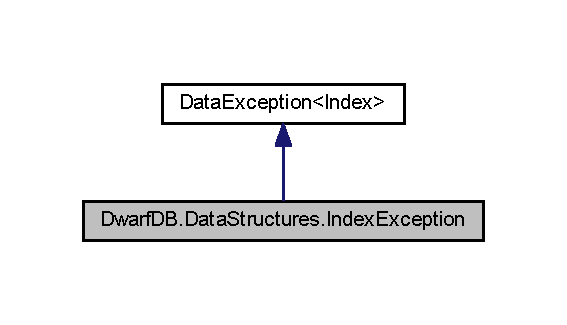
\includegraphics[width=272pt]{class_dwarf_d_b_1_1_data_structures_1_1_index_exception__coll__graph}
\end{center}
\end{figure}
\subsection*{Public Member Functions}
\begin{DoxyCompactItemize}
\item 
\hypertarget{class_dwarf_d_b_1_1_data_structures_1_1_index_exception_aee03e81543a53f20ddcca303c79018ad}{{\bfseries Index\+Exception} (string reason)}\label{class_dwarf_d_b_1_1_data_structures_1_1_index_exception_aee03e81543a53f20ddcca303c79018ad}

\item 
\hypertarget{class_dwarf_d_b_1_1_data_structures_1_1_index_exception_a2c9bcab774735ac2406f852f55647d46}{{\bfseries Index\+Exception} (\hyperlink{class_dwarf_d_b_1_1_data_structures_1_1_index}{Index} \+\_\+object, string reason)}\label{class_dwarf_d_b_1_1_data_structures_1_1_index_exception_a2c9bcab774735ac2406f852f55647d46}

\end{DoxyCompactItemize}
\subsection*{Additional Inherited Members}


The documentation for this class was generated from the following file\+:\begin{DoxyCompactItemize}
\item 
Data\+Structures/Data\+Exception.\+cs\end{DoxyCompactItemize}

\hypertarget{struct_dwarf_d_b_1_1_chunk_manager_1_1_index_pair}{\section{Dwarf\+D\+B.\+Chunk\+Manager.\+Index\+Pair Struct Reference}
\label{struct_dwarf_d_b_1_1_chunk_manager_1_1_index_pair}\index{Dwarf\+D\+B.\+Chunk\+Manager.\+Index\+Pair@{Dwarf\+D\+B.\+Chunk\+Manager.\+Index\+Pair}}
}
\subsection*{Static Public Member Functions}
\begin{DoxyCompactItemize}
\item 
\hypertarget{struct_dwarf_d_b_1_1_chunk_manager_1_1_index_pair_a66823af2deacc422dcac11403249dc52}{static int {\bfseries Sort} (string idx\+\_\+pattern, string foo)}\label{struct_dwarf_d_b_1_1_chunk_manager_1_1_index_pair_a66823af2deacc422dcac11403249dc52}

\end{DoxyCompactItemize}
\subsection*{Public Attributes}
\begin{DoxyCompactItemize}
\item 
\hypertarget{struct_dwarf_d_b_1_1_chunk_manager_1_1_index_pair_a703b8eeb5f0a8d55006a8df195130df7}{String {\bfseries hash\+\_\+min}}\label{struct_dwarf_d_b_1_1_chunk_manager_1_1_index_pair_a703b8eeb5f0a8d55006a8df195130df7}

\item 
\hypertarget{struct_dwarf_d_b_1_1_chunk_manager_1_1_index_pair_a0c8153c980b5a092260aa85d23e1b912}{String {\bfseries hash\+\_\+max}}\label{struct_dwarf_d_b_1_1_chunk_manager_1_1_index_pair_a0c8153c980b5a092260aa85d23e1b912}

\end{DoxyCompactItemize}


The documentation for this struct was generated from the following file\+:\begin{DoxyCompactItemize}
\item 
Chunk\+Manager/Chunk\+Manager.\+cs\end{DoxyCompactItemize}

\hypertarget{interface_dwarf_d_b_1_1_data_structures_1_1_i_structure}{
\section{DwarfDB.DataStructures.IStructure Interface Reference}
\label{interface_dwarf_d_b_1_1_data_structures_1_1_i_structure}\index{DwarfDB::DataStructures::IStructure@{DwarfDB::DataStructures::IStructure}}
}


An interface for DwarfDB data structures, such as: \hyperlink{class_dwarf_d_b_1_1_data_structures_1_1_data_container}{DataContainer} and \hyperlink{class_dwarf_d_b_1_1_data_structures_1_1_record}{Record}.  




Inheritance diagram for DwarfDB.DataStructures.IStructure:\nopagebreak
\begin{figure}[H]
\begin{center}
\leavevmode
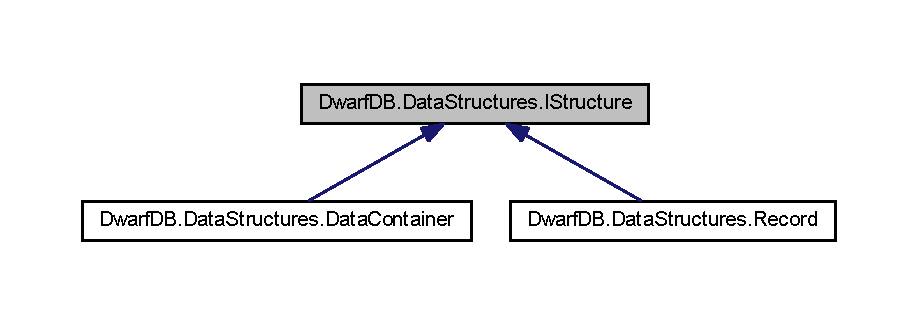
\includegraphics[width=400pt]{interface_dwarf_d_b_1_1_data_structures_1_1_i_structure__inherit__graph}
\end{center}
\end{figure}
\subsection*{Public Member Functions}
\begin{DoxyCompactItemize}
\item 
void \hyperlink{interface_dwarf_d_b_1_1_data_structures_1_1_i_structure_aa97bbd5250cf7456849fa6ca6ffcc0b4}{Save} ()
\begin{DoxyCompactList}\small\item\em Save to file chunk. \item\end{DoxyCompactList}\item 
void \hyperlink{interface_dwarf_d_b_1_1_data_structures_1_1_i_structure_acc1c091913384168ec50edad8b94b94b}{Load} (\hyperlink{class_dwarf_d_b_1_1_data_structures_1_1_index}{Index} index)
\begin{DoxyCompactList}\small\item\em Load Element from file chunk. \item\end{DoxyCompactList}\item 
void \hyperlink{interface_dwarf_d_b_1_1_data_structures_1_1_i_structure_a2e187a88a03b9e81e6e602be9329a395}{LoadFromChunkDir} (string dirpath, \hyperlink{class_dwarf_d_b_1_1_data_structures_1_1_index}{Index} index)
\begin{DoxyCompactList}\small\item\em Load Element from file chunk directory. \item\end{DoxyCompactList}\item 
void \hyperlink{interface_dwarf_d_b_1_1_data_structures_1_1_i_structure_aa89d0ecc5915538b89865bc3086d8b0a}{SetTransaction} (\hyperlink{class_dwarf_d_b_1_1_transactions_1_1_dwarf_transaction}{DwarfDB.Transactions.DwarfTransaction} InTransaction)
\begin{DoxyCompactList}\small\item\em Setting up a transaction for this element. \item\end{DoxyCompactList}\item 
\hyperlink{class_dwarf_d_b_1_1_data_structures_1_1_index}{Index} \hyperlink{interface_dwarf_d_b_1_1_data_structures_1_1_i_structure_a6fb14f0bf9df3268084bcc31dfd9c56f}{GetIndex} ()
\begin{DoxyCompactList}\small\item\em Getting an index for element. \item\end{DoxyCompactList}\item 
void \hyperlink{interface_dwarf_d_b_1_1_data_structures_1_1_i_structure_ae172c3eadf80027006666105c16b11ab}{BuildIndex} ()
\begin{DoxyCompactList}\small\item\em Building an index for element. \item\end{DoxyCompactList}\item 
\hyperlink{interface_dwarf_d_b_1_1_data_structures_1_1_i_structure}{IStructure} \hyperlink{interface_dwarf_d_b_1_1_data_structures_1_1_i_structure_a583485e1d898015ac75b952b057fb0e0}{Clone} ()
\begin{DoxyCompactList}\small\item\em Cloning procedure for DataStructure with reassigning a new owner object( for DC! ) \item\end{DoxyCompactList}\end{DoxyCompactItemize}
\subsection*{Properties}
\begin{DoxyCompactItemize}
\item 
Int64 \hyperlink{interface_dwarf_d_b_1_1_data_structures_1_1_i_structure_a20776b8ffebc8d77080ef4b9e9817e85}{Id}\hspace{0.3cm}{\ttfamily  \mbox{[}get, set\mbox{]}}
\begin{DoxyCompactList}\small\item\em Unique element id. \item\end{DoxyCompactList}\end{DoxyCompactItemize}


\subsection{Detailed Description}
An interface for DwarfDB data structures, such as: \hyperlink{class_dwarf_d_b_1_1_data_structures_1_1_data_container}{DataContainer} and \hyperlink{class_dwarf_d_b_1_1_data_structures_1_1_record}{Record}. 

\subsection{Member Function Documentation}
\hypertarget{interface_dwarf_d_b_1_1_data_structures_1_1_i_structure_ae172c3eadf80027006666105c16b11ab}{
\index{DwarfDB::DataStructures::IStructure@{DwarfDB::DataStructures::IStructure}!BuildIndex@{BuildIndex}}
\index{BuildIndex@{BuildIndex}!DwarfDB::DataStructures::IStructure@{DwarfDB::DataStructures::IStructure}}
\subsubsection[{BuildIndex}]{\setlength{\rightskip}{0pt plus 5cm}void DwarfDB.DataStructures.IStructure.BuildIndex (
\begin{DoxyParamCaption}
{}
\end{DoxyParamCaption}
)}}
\label{interface_dwarf_d_b_1_1_data_structures_1_1_i_structure_ae172c3eadf80027006666105c16b11ab}


Building an index for element. 



Implemented in \hyperlink{class_dwarf_d_b_1_1_data_structures_1_1_data_container_a8f32eb712d14d6dbf42a95098673dd19}{DwarfDB.DataStructures.DataContainer}, and \hyperlink{class_dwarf_d_b_1_1_data_structures_1_1_record_ab4ae005ad5474eb98a8aa45d7f8dd195}{DwarfDB.DataStructures.Record}.

\hypertarget{interface_dwarf_d_b_1_1_data_structures_1_1_i_structure_a583485e1d898015ac75b952b057fb0e0}{
\index{DwarfDB::DataStructures::IStructure@{DwarfDB::DataStructures::IStructure}!Clone@{Clone}}
\index{Clone@{Clone}!DwarfDB::DataStructures::IStructure@{DwarfDB::DataStructures::IStructure}}
\subsubsection[{Clone}]{\setlength{\rightskip}{0pt plus 5cm}{\bf IStructure} DwarfDB.DataStructures.IStructure.Clone (
\begin{DoxyParamCaption}
{}
\end{DoxyParamCaption}
)}}
\label{interface_dwarf_d_b_1_1_data_structures_1_1_i_structure_a583485e1d898015ac75b952b057fb0e0}


Cloning procedure for DataStructure with reassigning a new owner object( for DC! ) 

\begin{DoxyReturn}{Returns}

\end{DoxyReturn}


Implemented in \hyperlink{class_dwarf_d_b_1_1_data_structures_1_1_data_container_a246c00add5642b9674339a0319bae617}{DwarfDB.DataStructures.DataContainer}, and \hyperlink{class_dwarf_d_b_1_1_data_structures_1_1_record_a25e43ac7cdffc69c75cc466c859ce0ad}{DwarfDB.DataStructures.Record}.

\hypertarget{interface_dwarf_d_b_1_1_data_structures_1_1_i_structure_a6fb14f0bf9df3268084bcc31dfd9c56f}{
\index{DwarfDB::DataStructures::IStructure@{DwarfDB::DataStructures::IStructure}!GetIndex@{GetIndex}}
\index{GetIndex@{GetIndex}!DwarfDB::DataStructures::IStructure@{DwarfDB::DataStructures::IStructure}}
\subsubsection[{GetIndex}]{\setlength{\rightskip}{0pt plus 5cm}{\bf Index} DwarfDB.DataStructures.IStructure.GetIndex (
\begin{DoxyParamCaption}
{}
\end{DoxyParamCaption}
)}}
\label{interface_dwarf_d_b_1_1_data_structures_1_1_i_structure_a6fb14f0bf9df3268084bcc31dfd9c56f}


Getting an index for element. 

\begin{DoxyReturn}{Returns}

\end{DoxyReturn}


Implemented in \hyperlink{class_dwarf_d_b_1_1_data_structures_1_1_data_container_a195b9a3fcaa91d3240e07164c1d5c460}{DwarfDB.DataStructures.DataContainer}, and \hyperlink{class_dwarf_d_b_1_1_data_structures_1_1_record_abf7b1ed28e2f443a17f7658222b59c8f}{DwarfDB.DataStructures.Record}.

\hypertarget{interface_dwarf_d_b_1_1_data_structures_1_1_i_structure_acc1c091913384168ec50edad8b94b94b}{
\index{DwarfDB::DataStructures::IStructure@{DwarfDB::DataStructures::IStructure}!Load@{Load}}
\index{Load@{Load}!DwarfDB::DataStructures::IStructure@{DwarfDB::DataStructures::IStructure}}
\subsubsection[{Load}]{\setlength{\rightskip}{0pt plus 5cm}void DwarfDB.DataStructures.IStructure.Load (
\begin{DoxyParamCaption}
\item[{{\bf Index}}]{ index}
\end{DoxyParamCaption}
)}}
\label{interface_dwarf_d_b_1_1_data_structures_1_1_i_structure_acc1c091913384168ec50edad8b94b94b}


Load Element from file chunk. 


\begin{DoxyParams}{Parameters}
{\em filepath} & \\
\hline
{\em index} & \\
\hline
\end{DoxyParams}


Implemented in \hyperlink{class_dwarf_d_b_1_1_data_structures_1_1_data_container_ab045853ddb62b681d2474d7e547186de}{DwarfDB.DataStructures.DataContainer}, and \hyperlink{class_dwarf_d_b_1_1_data_structures_1_1_record_aba01a54cf8111326625980fd9b1d4d92}{DwarfDB.DataStructures.Record}.

\hypertarget{interface_dwarf_d_b_1_1_data_structures_1_1_i_structure_a2e187a88a03b9e81e6e602be9329a395}{
\index{DwarfDB::DataStructures::IStructure@{DwarfDB::DataStructures::IStructure}!LoadFromChunkDir@{LoadFromChunkDir}}
\index{LoadFromChunkDir@{LoadFromChunkDir}!DwarfDB::DataStructures::IStructure@{DwarfDB::DataStructures::IStructure}}
\subsubsection[{LoadFromChunkDir}]{\setlength{\rightskip}{0pt plus 5cm}void DwarfDB.DataStructures.IStructure.LoadFromChunkDir (
\begin{DoxyParamCaption}
\item[{string}]{ dirpath, }
\item[{{\bf Index}}]{ index}
\end{DoxyParamCaption}
)}}
\label{interface_dwarf_d_b_1_1_data_structures_1_1_i_structure_a2e187a88a03b9e81e6e602be9329a395}


Load Element from file chunk directory. 


\begin{DoxyParams}{Parameters}
{\em filepath} & \\
\hline
{\em index} & \\
\hline
\end{DoxyParams}


Implemented in \hyperlink{class_dwarf_d_b_1_1_data_structures_1_1_data_container_a0a82f79c53628134d16f2fa21db221bf}{DwarfDB.DataStructures.DataContainer}, and \hyperlink{class_dwarf_d_b_1_1_data_structures_1_1_record_a81ac5ba44d5682bfba61592af0195cd0}{DwarfDB.DataStructures.Record}.

\hypertarget{interface_dwarf_d_b_1_1_data_structures_1_1_i_structure_aa97bbd5250cf7456849fa6ca6ffcc0b4}{
\index{DwarfDB::DataStructures::IStructure@{DwarfDB::DataStructures::IStructure}!Save@{Save}}
\index{Save@{Save}!DwarfDB::DataStructures::IStructure@{DwarfDB::DataStructures::IStructure}}
\subsubsection[{Save}]{\setlength{\rightskip}{0pt plus 5cm}void DwarfDB.DataStructures.IStructure.Save (
\begin{DoxyParamCaption}
{}
\end{DoxyParamCaption}
)}}
\label{interface_dwarf_d_b_1_1_data_structures_1_1_i_structure_aa97bbd5250cf7456849fa6ca6ffcc0b4}


Save to file chunk. 


\begin{DoxyParams}{Parameters}
{\em filepath} & \\
\hline
\end{DoxyParams}


Implemented in \hyperlink{class_dwarf_d_b_1_1_data_structures_1_1_data_container_a3ca82caee7d6f38c74dbb4e2a637aecb}{DwarfDB.DataStructures.DataContainer}, and \hyperlink{class_dwarf_d_b_1_1_data_structures_1_1_record_a01889e57146fd3882228b09d2d54d51c}{DwarfDB.DataStructures.Record}.

\hypertarget{interface_dwarf_d_b_1_1_data_structures_1_1_i_structure_aa89d0ecc5915538b89865bc3086d8b0a}{
\index{DwarfDB::DataStructures::IStructure@{DwarfDB::DataStructures::IStructure}!SetTransaction@{SetTransaction}}
\index{SetTransaction@{SetTransaction}!DwarfDB::DataStructures::IStructure@{DwarfDB::DataStructures::IStructure}}
\subsubsection[{SetTransaction}]{\setlength{\rightskip}{0pt plus 5cm}void DwarfDB.DataStructures.IStructure.SetTransaction (
\begin{DoxyParamCaption}
\item[{{\bf DwarfDB.Transactions.DwarfTransaction}}]{ InTransaction}
\end{DoxyParamCaption}
)}}
\label{interface_dwarf_d_b_1_1_data_structures_1_1_i_structure_aa89d0ecc5915538b89865bc3086d8b0a}


Setting up a transaction for this element. 


\begin{DoxyParams}{Parameters}
{\em InTransaction} & \\
\hline
\end{DoxyParams}


Implemented in \hyperlink{class_dwarf_d_b_1_1_data_structures_1_1_data_container_a40b2dc31b54b0d41b29e58ea5ea4a3fb}{DwarfDB.DataStructures.DataContainer}, and \hyperlink{class_dwarf_d_b_1_1_data_structures_1_1_record_a4997c638afaaa5b8f281a492b639dfca}{DwarfDB.DataStructures.Record}.



\subsection{Property Documentation}
\hypertarget{interface_dwarf_d_b_1_1_data_structures_1_1_i_structure_a20776b8ffebc8d77080ef4b9e9817e85}{
\index{DwarfDB::DataStructures::IStructure@{DwarfDB::DataStructures::IStructure}!Id@{Id}}
\index{Id@{Id}!DwarfDB::DataStructures::IStructure@{DwarfDB::DataStructures::IStructure}}
\subsubsection[{Id}]{\setlength{\rightskip}{0pt plus 5cm}Int64 DwarfDB.DataStructures.IStructure.Id\hspace{0.3cm}{\ttfamily  \mbox{[}get, set\mbox{]}}}}
\label{interface_dwarf_d_b_1_1_data_structures_1_1_i_structure_a20776b8ffebc8d77080ef4b9e9817e85}


Unique element id. 



Implemented in \hyperlink{class_dwarf_d_b_1_1_data_structures_1_1_data_container_a3749f4fe324b56d46caf071488c615d7}{DwarfDB.DataStructures.DataContainer}, and \hyperlink{class_dwarf_d_b_1_1_data_structures_1_1_record_a6b9df97308b20ff8504cd88c56aded41}{DwarfDB.DataStructures.Record}.



The documentation for this interface was generated from the following file:\begin{DoxyCompactItemize}
\item 
DataStructures/IStructure.cs\end{DoxyCompactItemize}

\hypertarget{interface_dwarf_d_b_1_1_data_structures_1_1_i_structure_access}{\section{Dwarf\+D\+B.\+Data\+Structures.\+I\+Structure\+Access Interface Reference}
\label{interface_dwarf_d_b_1_1_data_structures_1_1_i_structure_access}\index{Dwarf\+D\+B.\+Data\+Structures.\+I\+Structure\+Access@{Dwarf\+D\+B.\+Data\+Structures.\+I\+Structure\+Access}}
}


Description of \hyperlink{interface_dwarf_d_b_1_1_data_structures_1_1_i_structure_access}{I\+Structure\+Access}.  




Inheritance diagram for Dwarf\+D\+B.\+Data\+Structures.\+I\+Structure\+Access\+:
\subsection*{Public Member Functions}
\begin{DoxyCompactItemize}
\item 
void \hyperlink{interface_dwarf_d_b_1_1_data_structures_1_1_i_structure_access_ace284cb4dcb438adf1482a657ab4cdf5}{Add\+Access} (\hyperlink{class_dwarf_d_b_1_1_user_1_1_user}{User.\+User} \+\_\+user, Dwarf\+D\+B.\+Access.\+Access.\+Access\+Level \+\_\+level)
\begin{DoxyCompactList}\small\item\em Adding a new access record \end{DoxyCompactList}\item 
void \hyperlink{interface_dwarf_d_b_1_1_data_structures_1_1_i_structure_access_acd6eb6c44eab3b1a8524983a1f7016a3}{Change\+Access} (\hyperlink{class_dwarf_d_b_1_1_user_1_1_user}{User.\+User} \+\_\+user, Access.\+Access.\+Access\+Level \+\_\+new\+\_\+level)
\begin{DoxyCompactList}\small\item\em Changing an access record \end{DoxyCompactList}\item 
Access.\+Access.\+Access\+Level \hyperlink{interface_dwarf_d_b_1_1_data_structures_1_1_i_structure_access_a3bc398d0e80fe5442502e6fa3c68d298}{Get\+Level} (\hyperlink{class_dwarf_d_b_1_1_user_1_1_user}{User.\+User} \+\_\+user)
\begin{DoxyCompactList}\small\item\em Getting an access level for a given user \end{DoxyCompactList}\end{DoxyCompactItemize}


\subsection{Detailed Description}
Description of \hyperlink{interface_dwarf_d_b_1_1_data_structures_1_1_i_structure_access}{I\+Structure\+Access}. 



\subsection{Member Function Documentation}
\hypertarget{interface_dwarf_d_b_1_1_data_structures_1_1_i_structure_access_ace284cb4dcb438adf1482a657ab4cdf5}{\index{Dwarf\+D\+B\+::\+Data\+Structures\+::\+I\+Structure\+Access@{Dwarf\+D\+B\+::\+Data\+Structures\+::\+I\+Structure\+Access}!Add\+Access@{Add\+Access}}
\index{Add\+Access@{Add\+Access}!Dwarf\+D\+B\+::\+Data\+Structures\+::\+I\+Structure\+Access@{Dwarf\+D\+B\+::\+Data\+Structures\+::\+I\+Structure\+Access}}
\subsubsection[{Add\+Access}]{\setlength{\rightskip}{0pt plus 5cm}void Dwarf\+D\+B.\+Data\+Structures.\+I\+Structure\+Access.\+Add\+Access (
\begin{DoxyParamCaption}
\item[{{\bf User.\+User}}]{\+\_\+user, }
\item[{Dwarf\+D\+B.\+Access.\+Access.\+Access\+Level}]{\+\_\+level}
\end{DoxyParamCaption}
)}}\label{interface_dwarf_d_b_1_1_data_structures_1_1_i_structure_access_ace284cb4dcb438adf1482a657ab4cdf5}


Adding a new access record 


\begin{DoxyParams}{Parameters}
{\em \+\_\+user} & \\
\hline
{\em \+\_\+level} & \\
\hline
\end{DoxyParams}


Implemented in \hyperlink{class_dwarf_d_b_1_1_data_structures_1_1_data_base_ab4f35460ca4de56345bffde22b2fc538}{Dwarf\+D\+B.\+Data\+Structures.\+Data\+Base}, and \hyperlink{class_dwarf_d_b_1_1_data_structures_1_1_data_container_ae4044ec9ce657af53ee87f365c2c6b89}{Dwarf\+D\+B.\+Data\+Structures.\+Data\+Container}.

\hypertarget{interface_dwarf_d_b_1_1_data_structures_1_1_i_structure_access_acd6eb6c44eab3b1a8524983a1f7016a3}{\index{Dwarf\+D\+B\+::\+Data\+Structures\+::\+I\+Structure\+Access@{Dwarf\+D\+B\+::\+Data\+Structures\+::\+I\+Structure\+Access}!Change\+Access@{Change\+Access}}
\index{Change\+Access@{Change\+Access}!Dwarf\+D\+B\+::\+Data\+Structures\+::\+I\+Structure\+Access@{Dwarf\+D\+B\+::\+Data\+Structures\+::\+I\+Structure\+Access}}
\subsubsection[{Change\+Access}]{\setlength{\rightskip}{0pt plus 5cm}void Dwarf\+D\+B.\+Data\+Structures.\+I\+Structure\+Access.\+Change\+Access (
\begin{DoxyParamCaption}
\item[{{\bf User.\+User}}]{\+\_\+user, }
\item[{Access.\+Access.\+Access\+Level}]{\+\_\+new\+\_\+level}
\end{DoxyParamCaption}
)}}\label{interface_dwarf_d_b_1_1_data_structures_1_1_i_structure_access_acd6eb6c44eab3b1a8524983a1f7016a3}


Changing an access record 


\begin{DoxyParams}{Parameters}
{\em \+\_\+user} & \\
\hline
{\em \+\_\+new\+\_\+level} & \\
\hline
\end{DoxyParams}


Implemented in \hyperlink{class_dwarf_d_b_1_1_data_structures_1_1_data_base_a4eaa522f122464c04a13d1ed104f6326}{Dwarf\+D\+B.\+Data\+Structures.\+Data\+Base}, and \hyperlink{class_dwarf_d_b_1_1_data_structures_1_1_data_container_a612995b0e084035ae6bcb7cb14b41f14}{Dwarf\+D\+B.\+Data\+Structures.\+Data\+Container}.

\hypertarget{interface_dwarf_d_b_1_1_data_structures_1_1_i_structure_access_a3bc398d0e80fe5442502e6fa3c68d298}{\index{Dwarf\+D\+B\+::\+Data\+Structures\+::\+I\+Structure\+Access@{Dwarf\+D\+B\+::\+Data\+Structures\+::\+I\+Structure\+Access}!Get\+Level@{Get\+Level}}
\index{Get\+Level@{Get\+Level}!Dwarf\+D\+B\+::\+Data\+Structures\+::\+I\+Structure\+Access@{Dwarf\+D\+B\+::\+Data\+Structures\+::\+I\+Structure\+Access}}
\subsubsection[{Get\+Level}]{\setlength{\rightskip}{0pt plus 5cm}Access.\+Access.\+Access\+Level Dwarf\+D\+B.\+Data\+Structures.\+I\+Structure\+Access.\+Get\+Level (
\begin{DoxyParamCaption}
\item[{{\bf User.\+User}}]{\+\_\+user}
\end{DoxyParamCaption}
)}}\label{interface_dwarf_d_b_1_1_data_structures_1_1_i_structure_access_a3bc398d0e80fe5442502e6fa3c68d298}


Getting an access level for a given user 


\begin{DoxyParams}{Parameters}
{\em \+\_\+user} & \\
\hline
\end{DoxyParams}
\begin{DoxyReturn}{Returns}

\end{DoxyReturn}


Implemented in \hyperlink{class_dwarf_d_b_1_1_data_structures_1_1_data_base_ade3f44a53526bbfbe698a18ca62e67a4}{Dwarf\+D\+B.\+Data\+Structures.\+Data\+Base}, and \hyperlink{class_dwarf_d_b_1_1_data_structures_1_1_data_container_ad268483590eb3c6db9f2a71519ab4b6c}{Dwarf\+D\+B.\+Data\+Structures.\+Data\+Container}.



The documentation for this interface was generated from the following file\+:\begin{DoxyCompactItemize}
\item 
Data\+Structures/I\+Structure\+Access.\+cs\end{DoxyCompactItemize}

\hypertarget{class_dwarf_d_b_1_1_transaction_journals_1_1_journal}{\section{Dwarf\+D\+B.\+Transaction\+Journals.\+Journal Class Reference}
\label{class_dwarf_d_b_1_1_transaction_journals_1_1_journal}\index{Dwarf\+D\+B.\+Transaction\+Journals.\+Journal@{Dwarf\+D\+B.\+Transaction\+Journals.\+Journal}}
}


Description of \hyperlink{namespace_dwarf_d_b_1_1_transaction_journals}{Transaction\+Journals}.  


\subsection*{Protected Attributes}
\begin{DoxyCompactItemize}
\item 
\hypertarget{class_dwarf_d_b_1_1_transaction_journals_1_1_journal_a804e9cfa2c0d03cc2b4ec5ffc1b25bf6}{List\\*
$<$ \hyperlink{interface_dwarf_d_b_1_1_data_structures_1_1_i_structure}{Dwarf\+D\+B.\+Data\+Structures.\+I\+Structure} $>$ {\bfseries journal\+\_\+objects} = new List$<$\hyperlink{interface_dwarf_d_b_1_1_data_structures_1_1_i_structure}{Dwarf\+D\+B.\+Data\+Structures.\+I\+Structure}$>$()}\label{class_dwarf_d_b_1_1_transaction_journals_1_1_journal_a804e9cfa2c0d03cc2b4ec5ffc1b25bf6}

\end{DoxyCompactItemize}


\subsection{Detailed Description}
Description of \hyperlink{namespace_dwarf_d_b_1_1_transaction_journals}{Transaction\+Journals}. 



The documentation for this class was generated from the following file\+:\begin{DoxyCompactItemize}
\item 
Transaction\+Journals/Transaction\+Journals.\+cs\end{DoxyCompactItemize}

\hypertarget{class_dwarf_d_b_1_1_program}{\section{Dwarf\+D\+B.\+Program Class Reference}
\label{class_dwarf_d_b_1_1_program}\index{Dwarf\+D\+B.\+Program@{Dwarf\+D\+B.\+Program}}
}
\subsection*{Static Public Member Functions}
\begin{DoxyCompactItemize}
\item 
\hypertarget{class_dwarf_d_b_1_1_program_ad191792c625399b2912062074ad4476b}{static void {\bfseries Main} (string\mbox{[}$\,$\mbox{]} args)}\label{class_dwarf_d_b_1_1_program_ad191792c625399b2912062074ad4476b}

\item 
\hypertarget{class_dwarf_d_b_1_1_program_af6bc5554955f41aa161cd638dd1fcbc1}{static void {\bfseries Data\+Base\+Chunk\+Creation} ()}\label{class_dwarf_d_b_1_1_program_af6bc5554955f41aa161cd638dd1fcbc1}

\item 
\hypertarget{class_dwarf_d_b_1_1_program_abab621dfeced1fb0c770bd5a1dffe3a6}{static void {\bfseries Data\+Table\+Chunk\+Creation} ()}\label{class_dwarf_d_b_1_1_program_abab621dfeced1fb0c770bd5a1dffe3a6}

\end{DoxyCompactItemize}


The documentation for this class was generated from the following files\+:\begin{DoxyCompactItemize}
\item 
Program.\+cs\item 
Samples/Data\+Base\+Test.\+cs\item 
Samples/Data\+Table\+Test.\+cs\end{DoxyCompactItemize}

\hypertarget{class_dwarf_d_b_1_1_data_structures_1_1_record}{\section{Dwarf\+D\+B.\+Data\+Structures.\+Record Class Reference}
\label{class_dwarf_d_b_1_1_data_structures_1_1_record}\index{Dwarf\+D\+B.\+Data\+Structures.\+Record@{Dwarf\+D\+B.\+Data\+Structures.\+Record}}
}


\hyperlink{class_dwarf_d_b_1_1_data_structures_1_1_record}{Record} is the element of \hyperlink{class_dwarf_d_b_1_1_data_structures_1_1_data_container}{Data\+Container}  




Inheritance diagram for Dwarf\+D\+B.\+Data\+Structures.\+Record\+:\nopagebreak
\begin{figure}[H]
\begin{center}
\leavevmode
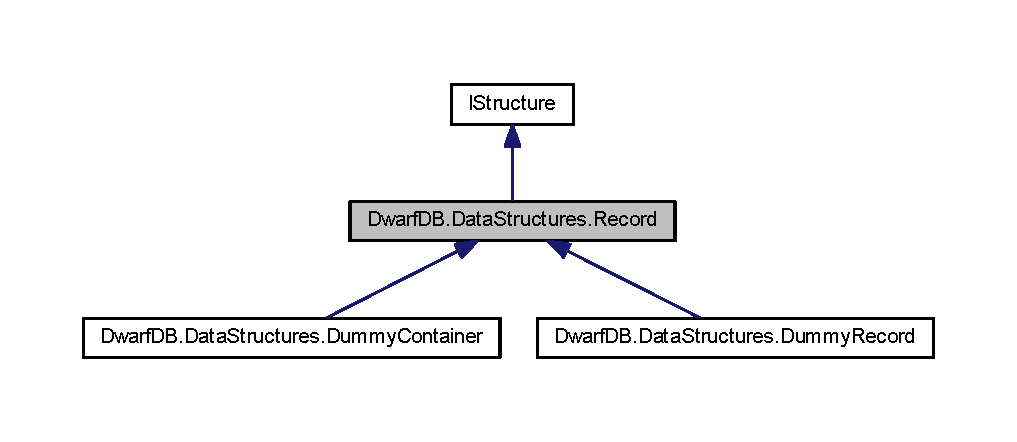
\includegraphics[width=236pt]{class_dwarf_d_b_1_1_data_structures_1_1_record__inherit__graph}
\end{center}
\end{figure}


Collaboration diagram for Dwarf\+D\+B.\+Data\+Structures.\+Record\+:\nopagebreak
\begin{figure}[H]
\begin{center}
\leavevmode
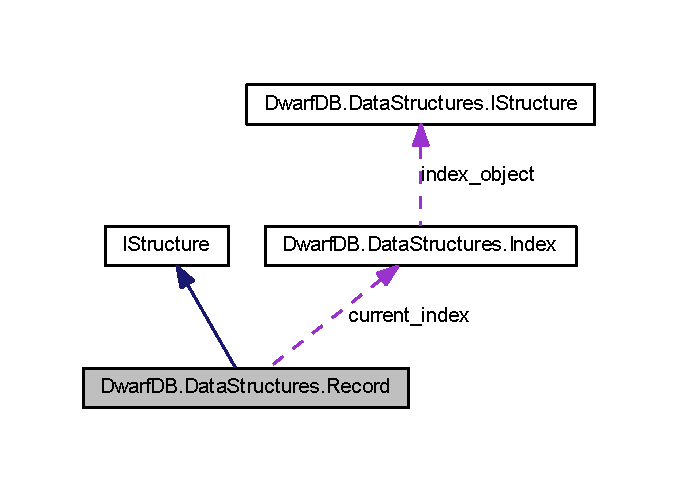
\includegraphics[width=325pt]{class_dwarf_d_b_1_1_data_structures_1_1_record__coll__graph}
\end{center}
\end{figure}
\subsection*{Public Member Functions}
\begin{DoxyCompactItemize}
\item 
\hypertarget{class_dwarf_d_b_1_1_data_structures_1_1_record_ac6bae5700b3a08e9903a5c592d810de0}{{\bfseries Record} (\hyperlink{class_dwarf_d_b_1_1_data_structures_1_1_data_container}{Data\+Container} \+\_\+owner\+\_\+dc)}\label{class_dwarf_d_b_1_1_data_structures_1_1_record_ac6bae5700b3a08e9903a5c592d810de0}

\item 
\hypertarget{class_dwarf_d_b_1_1_data_structures_1_1_record_a184d66ff6a8abfd88fc08aec61635295}{{\bfseries Record} (Serialization\+Info info, Streaming\+Context ctxt)}\label{class_dwarf_d_b_1_1_data_structures_1_1_record_a184d66ff6a8abfd88fc08aec61635295}

\item 
\hypertarget{class_dwarf_d_b_1_1_data_structures_1_1_record_ac10ee5af7dc2c00f831de89d0ac6592e}{void {\bfseries Get\+Object\+Data} (Serialization\+Info info, Streaming\+Context ctxt)}\label{class_dwarf_d_b_1_1_data_structures_1_1_record_ac10ee5af7dc2c00f831de89d0ac6592e}

\item 
void \hyperlink{class_dwarf_d_b_1_1_data_structures_1_1_record_a01889e57146fd3882228b09d2d54d51c}{Save} ()
\begin{DoxyCompactList}\small\item\em Save to file chunk \end{DoxyCompactList}\item 
void \hyperlink{class_dwarf_d_b_1_1_data_structures_1_1_record_aba01a54cf8111326625980fd9b1d4d92}{Load} (\hyperlink{class_dwarf_d_b_1_1_data_structures_1_1_index}{Index} index)
\begin{DoxyCompactList}\small\item\em Load Element from file chunk \end{DoxyCompactList}\item 
void \hyperlink{class_dwarf_d_b_1_1_data_structures_1_1_record_a4997c638afaaa5b8f281a492b639dfca}{Set\+Transaction} (\hyperlink{class_dwarf_d_b_1_1_transactions_1_1_dwarf_transaction}{Dwarf\+D\+B.\+Transactions.\+Dwarf\+Transaction} In\+Transaction)
\begin{DoxyCompactList}\small\item\em Setting up a transaction for this element \end{DoxyCompactList}\item 
\hyperlink{class_dwarf_d_b_1_1_data_structures_1_1_index}{Index} \hyperlink{class_dwarf_d_b_1_1_data_structures_1_1_record_abf7b1ed28e2f443a17f7658222b59c8f}{Get\+Index} ()
\begin{DoxyCompactList}\small\item\em Getting an index for element \end{DoxyCompactList}\item 
void \hyperlink{class_dwarf_d_b_1_1_data_structures_1_1_record_ab4ae005ad5474eb98a8aa45d7f8dd195}{Build\+Index} ()
\begin{DoxyCompactList}\small\item\em Building an index for element \end{DoxyCompactList}\item 
void \hyperlink{class_dwarf_d_b_1_1_data_structures_1_1_record_a81ac5ba44d5682bfba61592af0195cd0}{Load\+From\+Chunk\+Dir} (string dirpath, \hyperlink{class_dwarf_d_b_1_1_data_structures_1_1_index}{Index} index)
\begin{DoxyCompactList}\small\item\em Load \hyperlink{class_dwarf_d_b_1_1_data_structures_1_1_record}{Record} from file chunk directory \end{DoxyCompactList}\item 
\hypertarget{class_dwarf_d_b_1_1_data_structures_1_1_record_aefa85cab909d8d9b60aeabbb23bbc5c7}{void {\bfseries Reset} ()}\label{class_dwarf_d_b_1_1_data_structures_1_1_record_aefa85cab909d8d9b60aeabbb23bbc5c7}

\item 
\hypertarget{class_dwarf_d_b_1_1_data_structures_1_1_record_ad86f08f6a15fc5bef549031789a01ff8}{bool {\bfseries Move\+Next} ()}\label{class_dwarf_d_b_1_1_data_structures_1_1_record_ad86f08f6a15fc5bef549031789a01ff8}

\item 
\hypertarget{class_dwarf_d_b_1_1_data_structures_1_1_record_a17055913d08d7d28c235547f248d4540}{void {\bfseries Dispose} ()}\label{class_dwarf_d_b_1_1_data_structures_1_1_record_a17055913d08d7d28c235547f248d4540}

\item 
\hyperlink{interface_dwarf_d_b_1_1_data_structures_1_1_i_structure}{I\+Structure} \hyperlink{class_dwarf_d_b_1_1_data_structures_1_1_record_a25e43ac7cdffc69c75cc466c859ce0ad}{Clone} ()
\begin{DoxyCompactList}\small\item\em Cloning procedure for Data\+Structure with reassigning a new owner object( for D\+C! ) \end{DoxyCompactList}\item 
\hypertarget{class_dwarf_d_b_1_1_data_structures_1_1_record_afccd7c4257b4a7953265490700ca5d84}{void {\bfseries Assign\+Owner\+D\+C} (\hyperlink{class_dwarf_d_b_1_1_data_structures_1_1_data_container}{Data\+Container} \+\_\+owner\+\_\+dc)}\label{class_dwarf_d_b_1_1_data_structures_1_1_record_afccd7c4257b4a7953265490700ca5d84}

\end{DoxyCompactItemize}
\subsection*{Protected Attributes}
\begin{DoxyCompactItemize}
\item 
\hypertarget{class_dwarf_d_b_1_1_data_structures_1_1_record_a4db0f67a22a56cb80011e181956ac11e}{\hyperlink{class_dwarf_d_b_1_1_data_structures_1_1_index}{Index} {\bfseries current\+\_\+index}}\label{class_dwarf_d_b_1_1_data_structures_1_1_record_a4db0f67a22a56cb80011e181956ac11e}

\item 
\hypertarget{class_dwarf_d_b_1_1_data_structures_1_1_record_af547c3e838f95ede8120ec33ea410be2}{int {\bfseries position} = -\/1}\label{class_dwarf_d_b_1_1_data_structures_1_1_record_af547c3e838f95ede8120ec33ea410be2}

\end{DoxyCompactItemize}
\subsection*{Properties}
\begin{DoxyCompactItemize}
\item 
U\+Int64 \hyperlink{class_dwarf_d_b_1_1_data_structures_1_1_record_a6b33388f9fa7edcea1e29890da207be4}{Id}\hspace{0.3cm}{\ttfamily  \mbox{[}get, set\mbox{]}}
\begin{DoxyCompactList}\small\item\em Element id \end{DoxyCompactList}\item 
List$<$ \hyperlink{class_dwarf_d_b_1_1_data_structures_1_1_field}{Field} $>$ \hyperlink{class_dwarf_d_b_1_1_data_structures_1_1_record_ae901326df950b811aa2cbb5f632a21c3}{Fields}\hspace{0.3cm}{\ttfamily  \mbox{[}get\mbox{]}}
\begin{DoxyCompactList}\small\item\em List of fields \end{DoxyCompactList}\item 
\hyperlink{class_dwarf_d_b_1_1_data_structures_1_1_field}{Field} \hyperlink{class_dwarf_d_b_1_1_data_structures_1_1_record_a303a0895fdeb635fa47469b2ac46c4a3}{this\mbox{[}string field\+\_\+name\mbox{]}}\hspace{0.3cm}{\ttfamily  \mbox{[}get, set\mbox{]}}
\begin{DoxyCompactList}\small\item\em Getting fields and their values \end{DoxyCompactList}\item 
\hypertarget{class_dwarf_d_b_1_1_data_structures_1_1_record_adc6c66e17187956974f6102e89054528}{\hyperlink{class_dwarf_d_b_1_1_data_structures_1_1_data_container}{Data\+Container} {\bfseries Owner\+D\+C}\hspace{0.3cm}{\ttfamily  \mbox{[}get, set\mbox{]}}}\label{class_dwarf_d_b_1_1_data_structures_1_1_record_adc6c66e17187956974f6102e89054528}

\end{DoxyCompactItemize}


\subsection{Detailed Description}
\hyperlink{class_dwarf_d_b_1_1_data_structures_1_1_record}{Record} is the element of \hyperlink{class_dwarf_d_b_1_1_data_structures_1_1_data_container}{Data\+Container} 



\subsection{Member Function Documentation}
\hypertarget{class_dwarf_d_b_1_1_data_structures_1_1_record_ab4ae005ad5474eb98a8aa45d7f8dd195}{\index{Dwarf\+D\+B\+::\+Data\+Structures\+::\+Record@{Dwarf\+D\+B\+::\+Data\+Structures\+::\+Record}!Build\+Index@{Build\+Index}}
\index{Build\+Index@{Build\+Index}!Dwarf\+D\+B\+::\+Data\+Structures\+::\+Record@{Dwarf\+D\+B\+::\+Data\+Structures\+::\+Record}}
\subsubsection[{Build\+Index}]{\setlength{\rightskip}{0pt plus 5cm}void Dwarf\+D\+B.\+Data\+Structures.\+Record.\+Build\+Index (
\begin{DoxyParamCaption}
{}
\end{DoxyParamCaption}
)}}\label{class_dwarf_d_b_1_1_data_structures_1_1_record_ab4ae005ad5474eb98a8aa45d7f8dd195}


Building an index for element 



Implements \hyperlink{interface_dwarf_d_b_1_1_data_structures_1_1_i_structure_ae172c3eadf80027006666105c16b11ab}{Dwarf\+D\+B.\+Data\+Structures.\+I\+Structure}.

\hypertarget{class_dwarf_d_b_1_1_data_structures_1_1_record_a25e43ac7cdffc69c75cc466c859ce0ad}{\index{Dwarf\+D\+B\+::\+Data\+Structures\+::\+Record@{Dwarf\+D\+B\+::\+Data\+Structures\+::\+Record}!Clone@{Clone}}
\index{Clone@{Clone}!Dwarf\+D\+B\+::\+Data\+Structures\+::\+Record@{Dwarf\+D\+B\+::\+Data\+Structures\+::\+Record}}
\subsubsection[{Clone}]{\setlength{\rightskip}{0pt plus 5cm}{\bf I\+Structure} Dwarf\+D\+B.\+Data\+Structures.\+Record.\+Clone (
\begin{DoxyParamCaption}
{}
\end{DoxyParamCaption}
)}}\label{class_dwarf_d_b_1_1_data_structures_1_1_record_a25e43ac7cdffc69c75cc466c859ce0ad}


Cloning procedure for Data\+Structure with reassigning a new owner object( for D\+C! ) 

\begin{DoxyReturn}{Returns}

\end{DoxyReturn}


Implements \hyperlink{interface_dwarf_d_b_1_1_data_structures_1_1_i_structure_a583485e1d898015ac75b952b057fb0e0}{Dwarf\+D\+B.\+Data\+Structures.\+I\+Structure}.

\hypertarget{class_dwarf_d_b_1_1_data_structures_1_1_record_abf7b1ed28e2f443a17f7658222b59c8f}{\index{Dwarf\+D\+B\+::\+Data\+Structures\+::\+Record@{Dwarf\+D\+B\+::\+Data\+Structures\+::\+Record}!Get\+Index@{Get\+Index}}
\index{Get\+Index@{Get\+Index}!Dwarf\+D\+B\+::\+Data\+Structures\+::\+Record@{Dwarf\+D\+B\+::\+Data\+Structures\+::\+Record}}
\subsubsection[{Get\+Index}]{\setlength{\rightskip}{0pt plus 5cm}{\bf Index} Dwarf\+D\+B.\+Data\+Structures.\+Record.\+Get\+Index (
\begin{DoxyParamCaption}
{}
\end{DoxyParamCaption}
)}}\label{class_dwarf_d_b_1_1_data_structures_1_1_record_abf7b1ed28e2f443a17f7658222b59c8f}


Getting an index for element 

\begin{DoxyReturn}{Returns}

\end{DoxyReturn}


Implements \hyperlink{interface_dwarf_d_b_1_1_data_structures_1_1_i_structure_a6fb14f0bf9df3268084bcc31dfd9c56f}{Dwarf\+D\+B.\+Data\+Structures.\+I\+Structure}.



Here is the caller graph for this function\+:


\hypertarget{class_dwarf_d_b_1_1_data_structures_1_1_record_aba01a54cf8111326625980fd9b1d4d92}{\index{Dwarf\+D\+B\+::\+Data\+Structures\+::\+Record@{Dwarf\+D\+B\+::\+Data\+Structures\+::\+Record}!Load@{Load}}
\index{Load@{Load}!Dwarf\+D\+B\+::\+Data\+Structures\+::\+Record@{Dwarf\+D\+B\+::\+Data\+Structures\+::\+Record}}
\subsubsection[{Load}]{\setlength{\rightskip}{0pt plus 5cm}void Dwarf\+D\+B.\+Data\+Structures.\+Record.\+Load (
\begin{DoxyParamCaption}
\item[{{\bf Index}}]{index}
\end{DoxyParamCaption}
)}}\label{class_dwarf_d_b_1_1_data_structures_1_1_record_aba01a54cf8111326625980fd9b1d4d92}


Load Element from file chunk 


\begin{DoxyParams}{Parameters}
{\em filepath} & \\
\hline
{\em index} & \\
\hline
\end{DoxyParams}


Implements \hyperlink{interface_dwarf_d_b_1_1_data_structures_1_1_i_structure_acc1c091913384168ec50edad8b94b94b}{Dwarf\+D\+B.\+Data\+Structures.\+I\+Structure}.

\hypertarget{class_dwarf_d_b_1_1_data_structures_1_1_record_a81ac5ba44d5682bfba61592af0195cd0}{\index{Dwarf\+D\+B\+::\+Data\+Structures\+::\+Record@{Dwarf\+D\+B\+::\+Data\+Structures\+::\+Record}!Load\+From\+Chunk\+Dir@{Load\+From\+Chunk\+Dir}}
\index{Load\+From\+Chunk\+Dir@{Load\+From\+Chunk\+Dir}!Dwarf\+D\+B\+::\+Data\+Structures\+::\+Record@{Dwarf\+D\+B\+::\+Data\+Structures\+::\+Record}}
\subsubsection[{Load\+From\+Chunk\+Dir}]{\setlength{\rightskip}{0pt plus 5cm}void Dwarf\+D\+B.\+Data\+Structures.\+Record.\+Load\+From\+Chunk\+Dir (
\begin{DoxyParamCaption}
\item[{string}]{dirpath, }
\item[{{\bf Index}}]{index}
\end{DoxyParamCaption}
)}}\label{class_dwarf_d_b_1_1_data_structures_1_1_record_a81ac5ba44d5682bfba61592af0195cd0}


Load \hyperlink{class_dwarf_d_b_1_1_data_structures_1_1_record}{Record} from file chunk directory 


\begin{DoxyParams}{Parameters}
{\em filepath} & \\
\hline
{\em index} & \\
\hline
\end{DoxyParams}


Implements \hyperlink{interface_dwarf_d_b_1_1_data_structures_1_1_i_structure_a2e187a88a03b9e81e6e602be9329a395}{Dwarf\+D\+B.\+Data\+Structures.\+I\+Structure}.

\hypertarget{class_dwarf_d_b_1_1_data_structures_1_1_record_a01889e57146fd3882228b09d2d54d51c}{\index{Dwarf\+D\+B\+::\+Data\+Structures\+::\+Record@{Dwarf\+D\+B\+::\+Data\+Structures\+::\+Record}!Save@{Save}}
\index{Save@{Save}!Dwarf\+D\+B\+::\+Data\+Structures\+::\+Record@{Dwarf\+D\+B\+::\+Data\+Structures\+::\+Record}}
\subsubsection[{Save}]{\setlength{\rightskip}{0pt plus 5cm}void Dwarf\+D\+B.\+Data\+Structures.\+Record.\+Save (
\begin{DoxyParamCaption}
{}
\end{DoxyParamCaption}
)}}\label{class_dwarf_d_b_1_1_data_structures_1_1_record_a01889e57146fd3882228b09d2d54d51c}


Save to file chunk 


\begin{DoxyParams}{Parameters}
{\em filepath} & \\
\hline
\end{DoxyParams}


Implements \hyperlink{interface_dwarf_d_b_1_1_data_structures_1_1_i_structure_aa97bbd5250cf7456849fa6ca6ffcc0b4}{Dwarf\+D\+B.\+Data\+Structures.\+I\+Structure}.

\hypertarget{class_dwarf_d_b_1_1_data_structures_1_1_record_a4997c638afaaa5b8f281a492b639dfca}{\index{Dwarf\+D\+B\+::\+Data\+Structures\+::\+Record@{Dwarf\+D\+B\+::\+Data\+Structures\+::\+Record}!Set\+Transaction@{Set\+Transaction}}
\index{Set\+Transaction@{Set\+Transaction}!Dwarf\+D\+B\+::\+Data\+Structures\+::\+Record@{Dwarf\+D\+B\+::\+Data\+Structures\+::\+Record}}
\subsubsection[{Set\+Transaction}]{\setlength{\rightskip}{0pt plus 5cm}void Dwarf\+D\+B.\+Data\+Structures.\+Record.\+Set\+Transaction (
\begin{DoxyParamCaption}
\item[{{\bf Dwarf\+D\+B.\+Transactions.\+Dwarf\+Transaction}}]{In\+Transaction}
\end{DoxyParamCaption}
)}}\label{class_dwarf_d_b_1_1_data_structures_1_1_record_a4997c638afaaa5b8f281a492b639dfca}


Setting up a transaction for this element 


\begin{DoxyParams}{Parameters}
{\em In\+Transaction} & \\
\hline
\end{DoxyParams}


Implements \hyperlink{interface_dwarf_d_b_1_1_data_structures_1_1_i_structure_aa89d0ecc5915538b89865bc3086d8b0a}{Dwarf\+D\+B.\+Data\+Structures.\+I\+Structure}.



\subsection{Property Documentation}
\hypertarget{class_dwarf_d_b_1_1_data_structures_1_1_record_ae901326df950b811aa2cbb5f632a21c3}{\index{Dwarf\+D\+B\+::\+Data\+Structures\+::\+Record@{Dwarf\+D\+B\+::\+Data\+Structures\+::\+Record}!Fields@{Fields}}
\index{Fields@{Fields}!Dwarf\+D\+B\+::\+Data\+Structures\+::\+Record@{Dwarf\+D\+B\+::\+Data\+Structures\+::\+Record}}
\subsubsection[{Fields}]{\setlength{\rightskip}{0pt plus 5cm}List$<$ {\bf Field} $>$ Dwarf\+D\+B.\+Data\+Structures.\+Record.\+Fields\hspace{0.3cm}{\ttfamily [get]}}}\label{class_dwarf_d_b_1_1_data_structures_1_1_record_ae901326df950b811aa2cbb5f632a21c3}


List of fields 

\hypertarget{class_dwarf_d_b_1_1_data_structures_1_1_record_a6b33388f9fa7edcea1e29890da207be4}{\index{Dwarf\+D\+B\+::\+Data\+Structures\+::\+Record@{Dwarf\+D\+B\+::\+Data\+Structures\+::\+Record}!Id@{Id}}
\index{Id@{Id}!Dwarf\+D\+B\+::\+Data\+Structures\+::\+Record@{Dwarf\+D\+B\+::\+Data\+Structures\+::\+Record}}
\subsubsection[{Id}]{\setlength{\rightskip}{0pt plus 5cm}U\+Int64 Dwarf\+D\+B.\+Data\+Structures.\+Record.\+Id\hspace{0.3cm}{\ttfamily [get]}, {\ttfamily [set]}}}\label{class_dwarf_d_b_1_1_data_structures_1_1_record_a6b33388f9fa7edcea1e29890da207be4}


Element id 

\hypertarget{class_dwarf_d_b_1_1_data_structures_1_1_record_a303a0895fdeb635fa47469b2ac46c4a3}{\index{Dwarf\+D\+B\+::\+Data\+Structures\+::\+Record@{Dwarf\+D\+B\+::\+Data\+Structures\+::\+Record}!this\mbox{[}string field\+\_\+name\mbox{]}@{this[string field\+\_\+name]}}
\index{this\mbox{[}string field\+\_\+name\mbox{]}@{this[string field\+\_\+name]}!Dwarf\+D\+B\+::\+Data\+Structures\+::\+Record@{Dwarf\+D\+B\+::\+Data\+Structures\+::\+Record}}
\subsubsection[{this[string field\+\_\+name]}]{\setlength{\rightskip}{0pt plus 5cm}{\bf Field} Dwarf\+D\+B.\+Data\+Structures.\+Record.\+this\mbox{[}string field\+\_\+name\mbox{]}\hspace{0.3cm}{\ttfamily [get]}, {\ttfamily [set]}}}\label{class_dwarf_d_b_1_1_data_structures_1_1_record_a303a0895fdeb635fa47469b2ac46c4a3}


Getting fields and their values 



The documentation for this class was generated from the following file\+:\begin{DoxyCompactItemize}
\item 
Data\+Structures/Record.\+cs\end{DoxyCompactItemize}

\hypertarget{class_dwarf_d_b_1_1_unit_tests_1_1_record_test}{\section{Dwarf\+D\+B.\+Unit\+Tests.\+Record\+Test Class Reference}
\label{class_dwarf_d_b_1_1_unit_tests_1_1_record_test}\index{Dwarf\+D\+B.\+Unit\+Tests.\+Record\+Test@{Dwarf\+D\+B.\+Unit\+Tests.\+Record\+Test}}
}
\subsection*{Static Public Member Functions}
\begin{DoxyCompactItemize}
\item 
\hypertarget{class_dwarf_d_b_1_1_unit_tests_1_1_record_test_a907b0948a207c3deb0d62b1df26bf1f6}{static void {\bfseries Create\+Record} (string db\+\_\+name, string container\+\_\+name)}\label{class_dwarf_d_b_1_1_unit_tests_1_1_record_test_a907b0948a207c3deb0d62b1df26bf1f6}

\item 
\hypertarget{class_dwarf_d_b_1_1_unit_tests_1_1_record_test_af544fca880eb0a0bf19e6e0728c92c64}{static void {\bfseries Build\+Index} (string db\+\_\+name, string container\+\_\+name)}\label{class_dwarf_d_b_1_1_unit_tests_1_1_record_test_af544fca880eb0a0bf19e6e0728c92c64}

\end{DoxyCompactItemize}


The documentation for this class was generated from the following file\+:\begin{DoxyCompactItemize}
\item 
Unit\+Tests/Record\+Test.\+cs\end{DoxyCompactItemize}

\hypertarget{class_dwarf_d_b_1_1_user_1_1_user}{\section{Dwarf\+D\+B.\+User.\+User Class Reference}
\label{class_dwarf_d_b_1_1_user_1_1_user}\index{Dwarf\+D\+B.\+User.\+User@{Dwarf\+D\+B.\+User.\+User}}
}


Description of \hyperlink{class_dwarf_d_b_1_1_user_1_1_user}{User}.  


\subsection*{Static Public Member Functions}
\begin{DoxyCompactItemize}
\item 
static \hyperlink{class_dwarf_d_b_1_1_user_1_1_user}{User} \hyperlink{class_dwarf_d_b_1_1_user_1_1_user_acea2310c87e9c0606c9ee370e5946ea9}{Dummy} ()
\begin{DoxyCompactList}\small\item\em A user without any credentials and permissions \end{DoxyCompactList}\end{DoxyCompactItemize}
\subsection*{Properties}
\begin{DoxyCompactItemize}
\item 
\hypertarget{class_dwarf_d_b_1_1_user_1_1_user_ab59cfb6b9b4044adc4f20bb342bd0eef}{\hyperlink{class_dwarf_d_b_1_1_user_1_1_user_credentials}{User\+Credentials} {\bfseries Credentials}\hspace{0.3cm}{\ttfamily  \mbox{[}get\mbox{]}}}\label{class_dwarf_d_b_1_1_user_1_1_user_ab59cfb6b9b4044adc4f20bb342bd0eef}

\end{DoxyCompactItemize}


\subsection{Detailed Description}
Description of \hyperlink{class_dwarf_d_b_1_1_user_1_1_user}{User}. 



\subsection{Member Function Documentation}
\hypertarget{class_dwarf_d_b_1_1_user_1_1_user_acea2310c87e9c0606c9ee370e5946ea9}{\index{Dwarf\+D\+B\+::\+User\+::\+User@{Dwarf\+D\+B\+::\+User\+::\+User}!Dummy@{Dummy}}
\index{Dummy@{Dummy}!Dwarf\+D\+B\+::\+User\+::\+User@{Dwarf\+D\+B\+::\+User\+::\+User}}
\subsubsection[{Dummy}]{\setlength{\rightskip}{0pt plus 5cm}static {\bf User} Dwarf\+D\+B.\+User.\+User.\+Dummy (
\begin{DoxyParamCaption}
{}
\end{DoxyParamCaption}
)\hspace{0.3cm}{\ttfamily [static]}}}\label{class_dwarf_d_b_1_1_user_1_1_user_acea2310c87e9c0606c9ee370e5946ea9}


A user without any credentials and permissions 

\begin{DoxyReturn}{Returns}

\end{DoxyReturn}


The documentation for this class was generated from the following file\+:\begin{DoxyCompactItemize}
\item 
User/User.\+cs\end{DoxyCompactItemize}

\hypertarget{class_dwarf_d_b_1_1_user_1_1_user_credentials}{
\section{DwarfDB.User.UserCredentials Class Reference}
\label{class_dwarf_d_b_1_1_user_1_1_user_credentials}\index{DwarfDB::User::UserCredentials@{DwarfDB::User::UserCredentials}}
}


Class for user logins and password keeping.  


\subsection*{Public Attributes}
\begin{DoxyCompactItemize}
\item 
\hypertarget{class_dwarf_d_b_1_1_user_1_1_user_credentials_a709a6c58fefe81c94e4e57a045605747}{
string {\bfseries hashed\_\-pwd} = null}
\label{class_dwarf_d_b_1_1_user_1_1_user_credentials_a709a6c58fefe81c94e4e57a045605747}

\end{DoxyCompactItemize}
\subsection*{Properties}
\begin{DoxyCompactItemize}
\item 
\hypertarget{class_dwarf_d_b_1_1_user_1_1_user_credentials_a425f41d9c436edd834855475d5a7a554}{
String {\bfseries Login}\hspace{0.3cm}{\ttfamily  \mbox{[}get, set\mbox{]}}}
\label{class_dwarf_d_b_1_1_user_1_1_user_credentials_a425f41d9c436edd834855475d5a7a554}

\item 
\hypertarget{class_dwarf_d_b_1_1_user_1_1_user_credentials_ad74f3703718cd5f901e4b7fa0a704244}{
String {\bfseries Password}\hspace{0.3cm}{\ttfamily  \mbox{[}get, set\mbox{]}}}
\label{class_dwarf_d_b_1_1_user_1_1_user_credentials_ad74f3703718cd5f901e4b7fa0a704244}

\end{DoxyCompactItemize}


\subsection{Detailed Description}
Class for user logins and password keeping. 

The documentation for this class was generated from the following file:\begin{DoxyCompactItemize}
\item 
User/Credentials.cs\end{DoxyCompactItemize}

\hypertarget{class_dwarf_d_b_1_1_user_1_1_user_exception}{\section{Dwarf\+D\+B.\+User.\+User\+Exception Class Reference}
\label{class_dwarf_d_b_1_1_user_1_1_user_exception}\index{Dwarf\+D\+B.\+User.\+User\+Exception@{Dwarf\+D\+B.\+User.\+User\+Exception}}
}


Description of \hyperlink{class_dwarf_d_b_1_1_user_1_1_user_exception}{User\+Exception}.  




Inheritance diagram for Dwarf\+D\+B.\+User.\+User\+Exception\+:


Collaboration diagram for Dwarf\+D\+B.\+User.\+User\+Exception\+:
\subsection*{Public Member Functions}
\begin{DoxyCompactItemize}
\item 
\hypertarget{class_dwarf_d_b_1_1_user_1_1_user_exception_a1077457ad1927f13456743fa4829219b}{{\bfseries User\+Exception} (string message)}\label{class_dwarf_d_b_1_1_user_1_1_user_exception_a1077457ad1927f13456743fa4829219b}

\item 
\hypertarget{class_dwarf_d_b_1_1_user_1_1_user_exception_a4a3f2b2e90fa58f746465beda25bd0f8}{{\bfseries User\+Exception} (string message, Exception inner\+Exception)}\label{class_dwarf_d_b_1_1_user_1_1_user_exception_a4a3f2b2e90fa58f746465beda25bd0f8}

\end{DoxyCompactItemize}
\subsection*{Protected Member Functions}
\begin{DoxyCompactItemize}
\item 
\hypertarget{class_dwarf_d_b_1_1_user_1_1_user_exception_aadcc97ae25a3c4db279d96e721e9ef2a}{{\bfseries User\+Exception} (Serialization\+Info info, Streaming\+Context context)}\label{class_dwarf_d_b_1_1_user_1_1_user_exception_aadcc97ae25a3c4db279d96e721e9ef2a}

\end{DoxyCompactItemize}


\subsection{Detailed Description}
Description of \hyperlink{class_dwarf_d_b_1_1_user_1_1_user_exception}{User\+Exception}. 



The documentation for this class was generated from the following file\+:\begin{DoxyCompactItemize}
\item 
User/User\+Exception.\+cs\end{DoxyCompactItemize}

\hypertarget{class_dwarf_d_b_1_1_user_1_1_user_permissions}{\section{Dwarf\+D\+B.\+User.\+User\+Permissions Class Reference}
\label{class_dwarf_d_b_1_1_user_1_1_user_permissions}\index{Dwarf\+D\+B.\+User.\+User\+Permissions@{Dwarf\+D\+B.\+User.\+User\+Permissions}}
}


Description of Permissions.  




\subsection{Detailed Description}
Description of Permissions. 



The documentation for this class was generated from the following file\+:\begin{DoxyCompactItemize}
\item 
User/Permissions.\+cs\end{DoxyCompactItemize}

%--- End generated contents ---

% Index
\newpage
\phantomsection
\addcontentsline{toc}{chapter}{Index}
\printindex

\end{document}
